\documentclass[a4paper,12pt]{report}


%\usepackage[nottoc]{tocbibind}
%\usepackage{multirow}
 %\usepackage[backend=biber, style=numeric,]{biblatex}

%\DefineBibliographyStrings{french}{bibliography = {Webographie}}

%\addbibresource{allbiblio.bib}
%added%
\usepackage{csquotes}
\usepackage{pifont} % Pour utiliser les symboles de ding

\usepackage{amsmath}
\usepackage{amsfonts}
\usepackage{amssymb}
\usepackage{helvet}
\usepackage{graphicx}
\usepackage[frenchb]{babel} 
\usepackage{lipsum}
\usepackage{pdfpages}
%\usepackage{arabtex}
\usepackage[utf8]{inputenc}
\setcounter{secnumdepth}{10}

\usepackage{algorithmicx}
\usepackage[ruled]{algorithm}
\usepackage{algpseudocode}
\usepackage{enumitem}
\usepackage{float}
\usepackage{colortbl}
\usepackage[table, svgnames, dvipsnames]{xcolor}
\usepackage[justification=centering]{caption}
\captionsetup[figure]{font=small}
\usepackage[top=2.5cm, bottom=2.5cm, left=2.5cm, right=2.5cm]{geometry}
\usepackage{setspace}
\usepackage{fancyhdr}
\usepackage{minitoc}
%\setstretch{1.25}
%\usepackage[utf8x]{inputenc} %
\setcounter{tocdepth}{10}     % Dans la table des matieres
\usepackage{lettrine}

 \graphicspath{{figures//}}
 \usepackage{multicol}
% permet de faire une table des matieres par chapitre

% bibliographie par chapitre :
%     * mettre \bibliography et \bibliographystyle dans chaque fichier inclu
%\usepackage[sectionbib]{chapterbib}%
%\usepackage[french]{minitoc}   % permet de faire une table des matieres par chapitre
\usepackage{hyperref}
 \usepackage{fancyhdr}
 
 \pagestyle{fancy}
 
 \renewcommand{\headrulewidth}{1pt}
 \fancyhead[C]{\leftmark}
 \fancyhead[L]{}
 \fancyhead[R]{}
 
 \renewcommand{\footrulewidth}{1pt}
 \fancyfoot[C]{\textbf{page \thepage}} 
 \fancyfoot[L]{}
 \fancyfoot[R]{}

\newcommand{\HRule}{\rule{\linewidth}{0.5mm}}
\newcommand{\blap}[1]{\vbox to 0pt{#1\vss}}
\newcommand\AtUpperLeftCorner[3]{%
  \put(\LenToUnit{#1},\LenToUnit{\dimexpr\paperheight-#2}){\blap{#3}}%
}
\newcommand\AtUpperRightCorner[3]{%
  \put(\LenToUnit{\dimexpr\paperwidth-#1},\LenToUnit{\dimexpr\paperheight-#2}){\blap{\llap{#3}}}%
}
 
\begin{document} 
\hypersetup{hidelinks}


% preparation des minitocs

\onehalfspacing

\doparttoc
\pagenumbering{roman}




%\include{garde1.pdf}

\includepdf[pages=1]{garde1.pdf}

\includepdf[pages=2]{garde1.pdf}

\section*{Résumé }



{\bf Mots clefs : } 

%To start typing in Arabic use the command arabtext
\section*{Abstract}



{\bf Keywords:} Digital 
%\setcode{utf8}
%To start typing in Arabic use the command arabtext
  
 %To start typing in Arabic use the command arabtext




 

\chapter*{Remerciements}

Au terme de ce projet de fin d'études, je tiens à exprimer ma profonde gratitude envers toutes les personnes qui ont contribué, de près ou de loin, à l'aboutissement de ce travail.

Mes remerciements s'adressent tout d'abord à mon encadrant académique,\\ \textbf{Dr. Marouene CHAIEB}, pour sa disponibilité, ses conseils précieux et son suivi rigoureux tout au long de cette étape cruciale de ma formation.

Je tiens également à exprimer ma vive reconnaissance envers l'équipe de \textbf{PwC TAC Tunisie} pour m'avoir accueilli. Je remercie tout particulièrement ma maître de stage, \textbf{Mme Yoldez EL GAALOUL}, pour sa confiance, son expertise technique et son encadrement constant. Son soutien et l'environnement stimulant de PwC ont été déterminants dans ma découverte des solutions Salesforce et de l'intelligence artificielle.

Enfin, j'exprime ma gratitude aux membres du jury qui ont accepté d'évaluer ce travail et de m'honorer par leur présence.

À tous ceux qui ont rendu cette expérience enrichissante, merci.

\chapter*{Dédicaces}

\begin{center}
\it \large

À la mémoire de mes efforts et à l'aube de ma carrière, je dédie ce fruit de labeur :

\vspace{5mm}
\textbf{À mes très chers parents,}
Pour l'immensité de votre amour et la noblesse de vos sacrifices. Vos prières ont été mon bouclier et vos encouragements mon moteur. Que ce travail soit le reflet de l'éducation exemplaire que vous m'avez transmise.

\vspace{5mm}
\textbf{À mes sœurs,}
Pour votre complicité précieuse et votre soutien indéfectible. Vous avez su apaiser mes doutes et partager mes ambitions avec une bienveillance qui m'est chère.

\vspace{5mm}
\textbf{À mes collègues chez PwC,}
Pour votre accueil chaleureux, votre bienveillance et votre soutien technique précieux. Travailler à vos côtés a été une expérience enrichissante tant sur le plan professionnel qu'humain. Merci d'avoir partagé votre expertise et d'avoir contribué à la réussite de ce projet.

\vspace{5mm}
\textbf{À tous mes amis,}
Qui ont partagé de près ou de loin ce cheminement. Votre présence et votre fraternité resteront gravées dans mon esprit.

\vspace{8mm}
Puisse Dieu vous accorder santé, bonheur et longue vie.

\end{center}


\dominitoc
\tableofcontents
\listoffigures \mtcaddchapter
\listoftables  \mtcaddchapter


 %for openright
% inclusion des chapitres 
\chead{LISTE DES ABRÉVIATIONS} 
\chapter*{Liste des abréviations}

\begin{itemize}[label={}]
\item \textbf{XP} : Extreme Programming.
\item \textbf{UI} : User Interface. 
\item \textbf{UX} : User Experience. 
\item \textbf{IT} : Information Technology.
\item \textbf{SaaS} : Software as a Service.
\item \textbf{CNSS} : Caisse Nationale de Sécurité Sociale.
\item \textbf{ATS} : Applicant Tracking System.
\item \textbf{PERT} : Program Evaluation and Review Technique.
\item \textbf{NoSQL} : Not only SQL.
\item \textbf{JSON} : JavaScript Object Notation.
\item \textbf{API} : Application Programming Interface.
\item \textbf{REST} : Representational State Transfer.
\item \textbf{HTTP} : HyperText Transfer Protocol.
\item \textbf{CRUD} : Create, Read, Update, Delete.
\item \textbf{DTO} : Data Transfer Object.
\item \textbf{PME} : Petites et Moyennes Entreprises.

 
\end{itemize}

\pagenumbering{arabic}
\chead{INTRODUCTION GENERALE}

\setcounter{page}{1}

\chapter*{Introduction générale}
\addstarredchapter{Introduction générale}


Dans un contexte professionnel marqué par une transformation numérique accélérée, la gestion du recrutement s'impose comme un enjeu stratégique incontournable pour toute organisation soucieuse de sa compétitivité. Face à l'accroissement constant du volume des candidatures et à la complexité grandissante des processus de sélection, l'automatisation du recrutement est passée du statut d'avantage concurrentiel à celui de nécessité opérationnelle. C'est dans cette optique que s'inscrit notre projet de fin d'études, à travers la conception et le développement de SmartRec, une plateforme web intelligente entièrement dédiée à l'optimisation du processus de recrutement.
\par 
\textbf C'est dans cette logique que s'articule notre projet de fin d'études, à travers la conception et le développement de SmartRec, une plateforme web intelligente et évolutive. Ce projet a été mené au sein de l'entreprise PwC TAC Tunisie, avec l'objectif de proposer une solution innovante répondant aux besoins actuels des entreprises en matière de gestion et d'automatisation du recrutement.
\par 
\textbf SmartRec s'articule autour de deux profils utilisateurs aux prérogatives bien définies : le recruteur, qui gère les offres d'emploi, administre les comptes utilisateurs et consulte les dossiers de candidature avec leurs scores respectifs, et le candidat, qui parcourt les offres disponibles et soumet sa candidature via un formulaire interactif intelligent structuré en deux étapes distinctes.
\par 
\textbf Techniquement, SmartRec repose sur une architecture combinant Spring Boot, Angular et une base de données sécurisée, enrichie d'un modèle (NLP via SpaCy) assurant le parsing automatique des CVs et le calcul d'un score sur 100, le tout développé selon la méthodologie agile Scrum.
\par 
\textbf Ce rapport retrace l'ensemble des étapes suivies, de l'identification des besoins à la réalisation finale de la plateforme SmartRec, en mettant en avant les choix techniques, les défis rencontrés et les compétences mobilisées. Il est structuré pour refléter l'évolution du projet : le premier chapitre présente le cadre général du projet, suivi de l'analyse des besoins. Les chapitres suivants décrivent les sprints de développement, chacun portant sur un axe fonctionnel spécifique. Nous débuterons ainsi par une présentation du cadre général du projet, afin d'ancrer le lecteur dans son contexte de réalisation et ses objectifs initiaux.

\chead{CHAPITRE 1. CADRE GÉNÉRAL DU PROJET}
\chapter{ Cadre général du projet }

%\renewcommand{\mtctitle}{Sommaire}
\setcounter{mtc}{2}
\minitoc

\newpage
\section*{Introduction}

\addcontentsline{toc}{section}{\protect\numberline{}Introduction}
\par L'analyse de la situation actuelle est grandement influencée par l'étude préliminaire, qui se concentrera sur la définition des besoins. Ce chapitre couvre le cadre général du projet, en présentant brièvement l'organisme d'accueil, notre application web de recrutement intégrant un système de parsing de CV basé sur spaCy NLP et un scoring automatique, ainsi que la méthode de conduite de projet et les outils logiciels employés.

\vspace*{-0.5cm}

\section{Cadre du projet}
\hspace{0.5cm} \textbf Ce projet s'inscrit dans le cadre du travail de fin d'études en vue de l'obtention du diplôme de licence professionnelle en Business Computing, spécialité Business Information System, à ESPRIT School of Business (ESB), au cours de l'année universitaire 2024/2025. Ce stage a été effectué au sein de l'entreprise PwC TAC Tunisie, sous la supervision de Mme. Yoldez El Gaaloul, où nous avons développé une application web de recrutement intégrant des technologies intelligentes de parsing de CV et de scoring automatique.
\vspace*{-0.5cm}

\section{Présentation de l'organisme d'accueil}
Fondée en 1998 et implantée à Tunis, \textbf{PwC TAC Tunisie} est une filiale du réseau mondial PricewaterhouseCoopers, leader dans les services d'audit, de conseil et de fiscalité. Elle propose des solutions sur mesure dans les domaines de l'audit financier, du conseil en management et des services technologiques, au profit des entreprises locales et internationales opérant en Tunisie. Se distinguant par son engagement envers l'innovation et la transformation digitale, PwC TAC Tunisie constitue également un environnement privilégié pour le développement des jeunes talents au sein d'un réseau professionnel de renommée mondiale.

\vspace{0.3cm}
\begin{figure}[H]
\centering

\includegraphics[width=7cm, height=5cm]{Figures/PwC_logo.png}
\caption{Logo de la société "PriceWaterhouseCoopers TAC Tunisie"}\cite{beecoders_logo}
\end{figure}

\vspace{0.1cm}

\section{Etude de l'existant}
L'automatisation des processus de recrutement est devenue une nécessité incontournable pour les entreprises souhaitant optimiser leur gestion des ressources humaines. L'objectif de cette étude est d'analyser les solutions actuellement disponibles sur le marché afin d'identifier leurs forces et leurs limites, et ainsi justifier la nécessité d'un outil innovant tel que SmartRec. Ce dernier se distingue par son approche intelligente, intégrant des technologies de traitement du langage naturel (NLP via SpaCy) pour le parsing automatique des CVs des candidats, ainsi qu'un système de scoring automatisé permettant d'évaluer objectivement chaque candidat sur une échelle de 100 points, offrant ainsi aux recruteurs une expérience de gestion des candidatures plus efficace et plus précise.



\subsection{Description de l'existant}
Les solutions RH disponibles sur le marché, telles que \textbf{LinkedIn Jobs}, \textbf{Workday} et \textbf{Taleo}, demeurent insuffisantes dans une perspective globale. LinkedIn Jobs se limite à la publication d'offres, Workday reste coûteux et complexe, tandis que Taleo souffre d'une interface obsolète et d'un manque de fonctionnalités intelligentes. Aucune de ces plateformes n'exploite réellement l'intelligence artificielle pour optimiser les processus RH, ce qui justifie pleinement la création de \textbf{SmartRec}.

\subsection{Critique de l'existant }
Avant d'entamer le développement de SmartRec, il est primordial d'explorer le paysage concurrentiel existant, afin de mieux cerner les avantages et les insuffisances des outils déjà disponibles sur le marché. Cette analyse permet de s'appuyer sur les bonnes pratiques existantes tout en proposant des fonctionnalités distinctives et une réelle valeur ajoutée pour les recruteurs et les candidats.
\subsubsection{Linkedin}
 
LinkedIn Jobs est une plateforme mondiale de recrutement en ligne, spécialisée dans la mise en relation entre recruteurs et candidats. Elle permet aux entreprises de publier des offres d'emploi, de consulter les profils des candidats et de gérer les candidatures reçues grâce à une interface web intuitive et des outils de recherche avancés.
 \cite{esperoo2025}
\vspace{0.3cm}

\begin{figure}[H]
\centering
\fbox{
\includegraphics[width=3cm, height=3cm]{Figures/logo_linkedin.png}}
\caption{Logo de site web "Linkedin"}\cite{logo_linkedin}
\label{SEIF}
\end{figure}



\vspace{0.1cm}
Voici ce que nous avons pu observer comme points forts et points à améliorer dans cette application.
\vspace{0.2cm}
\\
\\
\par \underline{\textbf{Points Forts}}\\

\begin{itemize}[label=\textbullet]

 \item[\ding{51}] \textbf{Suivi précis du temps de travail :}LinkedIn Jobs se distingue par sa capacité à connecter les recruteurs avec des millions de candidats à travers le monde, offrant ainsi un accès à une base de données étendue de profils professionnels variés et qualifiés.
 
\item[\ding{51}] \textbf{Planification optimisée :} Elle facilite la publication d'offres d'emploi claires et ciblées, adaptées aux besoins et aux exigences de chaque entreprise.

\item[\ding{51}]  \textbf{Interface locale :} La plateforme est adaptée aux besoins des entreprises de toutes tailles, qu'elles soient locales ou internationales, grâce à ses outils de recrutement flexibles et personnalisables.

\end{itemize}

\par \underline{\textbf{Points Faibles}}\\
\begin{itemize}[label=\textbullet]

\item[\ding{56}]  \textbf{Absence de fonctionnalités intelligentes : } Aucun système de parsing automatique des CVs ni de scoring automatisé des candidats n'est intégré, ce qui oblige les recruteurs à évaluer manuellement chaque candidature reçue.

\item[\ding{56}]  \textbf{Absence de gestion des candidatures avancée :} Il n'est pas possible de filtrer, classer ou scorer automatiquement les candidats selon leurs compétences et leur adéquation avec le poste proposé.
\item[\ding{56}]  \textbf{Absence de gestion des CVs :} Il n'existe pas d'espace dédié au stockage et à l'analyse automatique des CVs des candidats, ce qui complique la consultation et le suivi des dossiers de candidature par les recruteurs.

\end{itemize}

\subsubsection{Workday Recruiting}
Workday Recruiting est une solution SaaS mondiale de gestion du recrutement, intégrée au sein de la suite RH de Workday. Elle propose un système automatisé pour la publication des offres d'emploi et la gestion des candidatures, avec un suivi des candidats et un tableau de bord centralisé permettant aux recruteurs de piloter efficacement leur processus de recrutement.

\cite{WorkDay}
\vspace{0.3cm}

\begin{figure}[H]
\centering
\fbox{
\includegraphics[width=11cm, height=2cm]{Figures/workday_logo.png}}
\caption{Logo de platform "WorkDay" }\cite{workday_logo}
\label{fig:planification}
\end{figure}



\vspace{0.2cm}
Voici ce que nous avons pu observer comme points forts et points à améliorer dans cette application.

\par \underline{\textbf{Points Forts}}\\
\begin{itemize}[label=\textbullet]
\item[\ding{51}]  \textbf{Facilité d'utilisation :} La plateforme dispose d'une interface claire et ergonomique, ce qui permet aux recruteurs et aux responsables RH de la prendre en main rapidement et sans difficultés.
\item[\ding{51}]  \textbf{Automatisation du processus de recrutement : } Le suivi des candidatures est fluide et structuré, avec des notifications automatiques envoyées aux recruteurs et aux candidats, assurant ainsi une traçabilité complète de chaque étape du processus de recrutement.
\item[\ding{51}]  \textbf{Adapté aux grandes entreprises :} Sa mise en œuvre rapide et ses fonctionnalités avancées en font une solution bien adaptée aux entreprises de grande taille souhaitant optimiser et centraliser leur processus de recrutement.
\end{itemize}

\par \underline{\textbf{Points Faibles}}\\
\begin{itemize}[label=\textbullet]
\item[\ding{56}]  \textbf{Absence de fonctionnalités intelligentes : }Aucune fonctionnalité liée au parsing automatique des CVs ou au scoring automatisé des candidats n'est disponible, ce qui oblige les recruteurs à évaluer manuellement chaque dossier de candidature.
\item[\ding{56}]  \textbf{Absence d'analyse des candidats :}  La plateforme ne permet pas d'évaluer automatiquement les compétences, l'expérience ou le niveau d'adéquation des candidats par rapport au poste proposé.
\item[\ding{56}]  \textbf{Manque de flexibilité : } L'outil reste limité dans ses options de personnalisation et ne s'adapte pas facilement aux besoins spécifiques de chaque entreprise en matière de recrutement.

\end{itemize}

\subsubsection{ Taleo  }
Taleo est une plateforme de recrutement américaine développée par Oracle, reconnue mondialement et utilisée par de nombreuses entreprises de grande taille. Elle permet de centraliser la gestion des offres d'emploi, le suivi des candidatures et la gestion des talents, grâce à une interface complète et des outils performants dédiés aux équipes RH.
\cite{Taleo}
\vspace{0.3cm}

\begin{figure}[H]
\centering
\fbox{
\includegraphics[width=3cm, height=3cm]{Figures/Taleo_logol.jpg}}
\caption{Logo de platform "NGES RH"}\cite{Taleo_logo}
\label{fig:planification}
\end{figure}

\vspace{0.2cm}
Voici ce que nous avons pu observer comme points forts et points à améliorer dans cette application.

\par \underline{\textbf{Points Forts}}\\
\begin{itemize}[label=\textbullet]
\item[\ding{51}]  \textbf{Gestion complète du recrutement :} La plateforme assure une prise en charge intégrale des différentes étapes du processus d'embauche, allant de la diffusion des offres d'emploi jusqu'à la sélection finale des candidats les plus qualifiés.
\item[\ding{51}]  \textbf{Déploiement à l'échelle mondiale: } Il est conforme aux exigences réglementaires tunisiennes (ex. : CNSS, bulletins de paie).La plateforme est utilisée par des entreprises dans de nombreux pays, ce qui lui permet de s'adapter aux différentes exigences et aux contextes variés des organisations à travers le monde.
\item[\ding{51}]  \textbf{Disponibilité d'un module de recrutement avancé :} La plateforme intègre un système complet de gestion des candidatures, offrant aux recruteurs un suivi détaillé et structuré de chaque candidat tout au long du processus de sélection.
\end{itemize}

\par \underline{\textbf{Points Faibles}}\\
\begin{itemize}[label=\textbullet]
\item[\ding{56}]  \textbf{Fonctionnalités de recrutement limitées : } Bien que la plateforme dispose d'un module de recrutement, celui-ci reste insuffisant car il ne propose ni parsing automatique des CVs, ni scoring automatisé des candidats, ni analyse intelligente des dossiers de candidature.
\item[\ding{56}]  \textbf{Manque de collaboration entre recruteurs : } La plateforme ne permet pas aux membres de l'équipe RH de partager des avis, d'échanger des commentaires ou de travailler conjointement sur l'évaluation des candidats.
\item[\ding{56}]  \textbf{Interface utilisateur complexe:} Taleo possède une interface vieillissante et peu intuitive, nécessitant une formation approfondie, ce qui ralentit le processus de recrutement.
\end{itemize}

\subsection{Solution proposée:}
C’est précisément pour pallier l’ensemble de ces insuffisances que SmartRec a été
conçu. Ce projet ambitionne de fournir une solution moderne, intelligente et adaptée aux
exigences du marché actuel. À la différence des outils existants, fréquemment cantonnés à
une fonctionnalité unique ou dépourvus d’innovation technologique, SmartRec rassemble
en une seule plateforme cohérente et performante l’ensemble des services indispensables à
une gestion efficace du recrutement. Plusieurs éléments fondamentaux distinguent SmartRec de la concurrence :

\textbullet \hspace{0.2cm} \textbf {recrutement intelligent et optimisé : } SmartRec propose un module exhaustif couvrant la publication des offres, la réception des candidatures ainsi qu'un mécanisme de sélection automatisé reposant sur un scoring avancé et une analyse approfondie des CVs.

\textbullet \hspace{0.2cm} \textbf{ collaboration active au sein des équipes RH : } la plateforme offre un environnement de travail collaboratif permettant aux recruteurs de partager leurs évaluations, d'échanger leurs retours et de statuer collectivement sur les profils des candidats.



\textbullet \hspace{0.2cm} \textbf{Une exploitation réelle de l'intelligence artificielle:} contrairement aux solutions concurrentes, SmartRec intègre l'IA au cœur de ses processus afin d'automatiser l'analyse des dossiers, d'affiner le scoring des candidats et d'améliorer la qualité des décisions de recrutement.

\textbullet \hspace{0.2cm} \textbf{Sécurité et ergonomie : } un contrôle rigoureux des accès selon les rôles des utilisateurs, associé à une interface fluide, réactive et intuitive, garantit une expérience utilisateur optimale.



\subsection{Justification du choix d’un site web de Recrutement}

Dans un contexte professionnel marqué par des mutations profondes et continues, la transformation numérique des fonctions RH s'est progressivement imposée comme un impératif stratégique pour toute organisation aspirant à renforcer son efficacité opérationnelle et à consolider sa position concurrentielle. Le déploiement d'une plateforme web spécialisée dans la gestion des ressources humaines constitue dès lors une démarche innovante et résolument tournée vers l'avenir, offrant la possibilité de regrouper l'ensemble des opérations RH au sein d'un dispositif unique et intégré. Une telle centralisation présente des avantages multiples et significatifs : elle permet notamment d'automatiser des tâches administratives répétitives et chronophages, à l'instar de la gestion des absences, du suivi des présences ou de la conduite du processus de recrutement, contribuant ainsi à réduire considérablement les risques d'erreurs humaines tout en permettant aux équipes de se consacrer pleinement à des activités à plus forte valeur ajoutée. En outre, ce type de solution favorise une communication interne plus fluide et transparente, en donnant aux collaborateurs comme aux responsables RH un accès simplifié et structuré aux informations dont ils ont besoin. Elle représente également un gage de conformité aux obligations légales et réglementaires en vigueur. C'est animé par ces convictions que SmartRec a été développé, avec la volonté affirmée de proposer une solution complète, ergonomique et performante, capable d'accompagner durablement les entreprises dans la valorisation et la gestion optimale de leur capital humain.



\section{Méthodologie adoptée}
\par 
La réussite d'un projet informatique ne saurait se réduire aux seuls choix technologiques opérés, mais repose fondamentalement sur la qualité de son pilotage et la rigueur de son organisation. Une conduite de projet véritablement efficace implique une vision stratégique clairement définie, une démarche structurée et réfléchie, ainsi que des décisions fondées sur des données concrètes et fiables. C'est dans cette perspective que le développement de SmartRec a été mené en adoptant la méthodologie Scrum, reconnue pour sa clarté et sa simplicité de mise en œuvre. De façon générale, il est possible de distinguer deux grandes familles de méthodologies de conduite de projet :
	\begin{itemize}[label=\textbullet]
\textbullet \hspace{0.2cm} \textbf {Les approches traditionnelles ou prédictives : } ces méthodes reposent sur une planification exhaustive et séquentielle établie en amont, où chaque étape est définie avant le lancement du projet, offrant ainsi peu de marge pour d'éventuels ajustements en cours de développement\\
\textbullet \hspace{0.2cm} \textbf {Les méthodes agiles : } à l'inverse, ces approches privilégient la flexibilité, l'interaction permanente entre les membres de l'équipe et l'amélioration continue du produit, permettant une adaptation rapide et efficace face aux évolutions et aux besoins émergents.
    \end{itemize}



\subsection{Méthodes classiques}
Les méthodes classiques telles que le modèle en cascade et le cycle en V reposent sur une logique séquentielle stricte, où chaque phase doit être achevée avant de passer à la suivante. Bien qu'elles offrent un cadre structuré, leur rigidité et leur manque de flexibilité les rendent inadaptées aux projets nécessitant des ajustements fréquents et une évolution continue.
\subsubsection{Présentation des méthodes classiques }
Les méthodes classiques, également désignées sous le terme de méthodes prédictives, se caractérisent par une planification minutieuse établie en amont et une exécution strictement linéaire du projet. Ce dernier progresse de manière séquentielle à travers des phases bien définies, à savoir l'analyse, la conception, le développement, les tests et le déploiement, chacune devant être intégralement finalisée avant d'entamer la suivante. Parmi les approches les plus répandues, on distingue :

\textbullet \hspace{0.2cm} \textbf{Le cycle en V :} largement utilisé en informatique, il repose sur une validation systématique à chaque étape, garantissant une traçabilité rigoureuse mais imposant une structure particulièrement inflexible.

\textbullet \hspace{0.2cm} \textbf{La méthode Waterfall :} fondée sur une progression unidirectionnelle, cette approche ne permet aucun retour en arrière une fois une phase achevée, la rendant adaptée uniquement aux projets aux exigences stables et bien définies.

\textbullet \hspace{0.2cm} \textbf{Les méthodes PERT et Gantt :} outils de planification complémentaires, le diagramme de Gantt visualise l'enchaînement des tâches dans le temps, tandis que PERT permet d'identifier les chemins critiques et d'anticiper les risques de retard.
    
\subsubsection{Insuffisances des approches traditionnelles }
 
En dépit de leur cadre organisationnel structuré, les méthodes classiques révèlent plusieurs insuffisances majeures lorsqu'elles sont confrontées aux exigences des projets modernes et évolutifs. Parmi les faiblesses les plus significatives, on peut relever :
	
	\begin{itemize}[label=\textbullet]
	\item	\textbf{Une rigidité contraignante :  }difficile d’adapter le projet en cours de route si les besoins changent.
    \item \textbf{Une visibilité tardive du produit :} Le produit final n’est visible qu’à la fin, ce qui peut générer des écarts par rapport aux attentes.
    
    \item \textbf{Une détection différée des anomalies :} Les erreurs découvertes en fin de cycle sont coûteuses à corriger.
    \item	\textbf{Des échanges limités au sein de l'équipe :}les échanges entre les équipes sont limités, ce qui freine l’adaptation et l’innovation.

    \item	\textbf{Une déconnexion des attentes réelles:} les spécifications sont parfois déconnectées des attentes des utilisateurs finaux.



	\end{itemize}

 \subsection{Naissance des approches agiles }
Afin de saisir pleinement l'engouement croissant des organisations pour les méthodes agiles, il convient de remonter aux fondements historiques qui ont présidé à leur émergence. C'est en février 2001 que dix-sept experts reconnus du développement logiciel se sont réunis à Snowbird, dans l'Utah aux États-Unis, animés par la volonté commune de repenser les pratiques existantes et de dépasser les limites inhérentes aux méthodes traditionnelles. De cette rencontre fondatrice est né le célèbre Manifeste Agile, qui a posé les valeurs cardinales de l'agilité :

	\begin{itemize}[label=\textbullet]
	\item La primauté des interactions humaines sur les processus formalisés et les outils techniques,
 	\item Un logiciel opérationnel plutôt qu'une documentation exhaustive et figée,
    \item Une relation de confiance avec le client qui prime sur les contraintes contractuelles,
 	\item La capacité d'adaptation aux changements qui l'emporte sur le respect rigide d'un plan préétabli.
		\end{itemize}
        \vspace{0.2cm}
		\par Ce manifeste fondateur s'appuie également sur douze principes directeurs promouvant la transparence, l'autonomie des équipes, la livraison rapide et continue de valeur, ainsi que la satisfaction permanente du client. Depuis lors, les méthodes agiles ont connu une diffusion remarquable, s'étendant bien au-delà de la sphère informatique pour irriguer l'ensemble des domaines de la gestion de projet.



\subsection{Choix de méthodologie : SCRUM} 
Dans le domaine du développement logiciel, plusieurs méthodes agiles ont émergé pour rendre la gestion de projet plus souple et mieux adaptée aux besoins réels des utilisateurs. Bien qu’elles reposent sur les mêmes valeurs, chaque méthode a ses spécificités et ses avantages. Parmi les plus répandues, on retrouve :

\textbullet \hspace{0.2cm} \textbf{ Scrum : }articulée autour de cycles itératifs courts appelés sprints, cette méthode instaure une organisation rigoureuse des rôles et favorise une livraison régulière de valeur.

\textbullet \hspace{0.2cm} \textbf{XP (Extreme Programming) :} orientée vers l'excellence technique, elle privilégie des pratiques telles que les tests automatisés et l'intégration continue afin de garantir la qualité du code produit.

\textbullet \hspace{0.2cm} \textbf{Kanban :} reposant sur une représentation visuelle des flux de travail, elle assure un suivi continu et transparent de l'avancement des tâches via un tableau dynamique.

\begin{table}[H]
\begin{center}
\captionsetup{justification=centering}
 \caption{\label{tab:<< Tableau comparatif – Méthodes agiles >>} Tableau comparatif des méthodes agiles  }
\begin{tabular}{|p{2cm}|p{7.5cm}|p{6.5cm}|} \arrayrulecolor{black}\rowcolor{WhiteSmoke}
\hline 
\textbf{Méthode} &
\hspace*{1.5cm} \textbf{Points Forts} &
 \hspace*{1cm} \textbf{Points Faibles} \\ \hline
\textbf{SCRUM} &
  \begin{tabular}[c]{@{}l@{}}• Organisation claire des rôles (Product \\ Owner, Scrum Master, équipe).\\ •Progression visible grâce aux sprints \\itératifs \\ • Communication fluide et ajustements \\réguliers \end{tabular} &
  \begin{tabular}[c]{@{}l@{}}• Peut devenir contraignant si les \\rôles ne sont pas rigoureusement\\ respectés.\\• Nécessite une équipe \\préalablement formée à la méthode. \end{tabular} \\ \hline
\textbf{XP} &
  \begin{tabular}[c]{@{}l@{}}• Privilégie une qualité élevée du code.\\• Intégration systématique de tests\\ automatisés \\• Encourage la collaboration étroite entre \\développeurs.
  \end{tabular} &
  \begin{tabular}[c]{@{}l@{}}• Exige un niveau technique avancé\\ et une grande rigueur.\\•  Peu adapté aux équipes \\nombreuses ou aux environnements\\ très formalisés.\end{tabular} \\ \hline
\textbf{Kanban} &
  \begin{tabular}[c]{@{}l@{}}• Mise en place simple et rapide. \\• Visualisation intuitive via un tableau de \\bord. \\• Grande souplesse et réactivité face aux\\ imprévus. \end{tabular} &
  \begin{tabular}[c]{@{}l@{}}• N'impose aucune structure\\ temporelle ni itérative.\\•Offre une vision globale\\ insuffisante pour les projets\\ complexes.\end{tabular} \\ \hline
\end{tabular}

\end{center}
\end{table}
L'examen du tableau comparatif révèle que Scrum constitue le choix le plus judicieux pour \textbf{SmartRec}. Kanban, bien que souple, manque de cadre structurant, tandis que XP privilégie la technique au détriment des besoins fonctionnels. Scrum offre ainsi un équilibre optimal entre rigueur organisationnelle, clarté des rôles et capacité d'adaptation, répondant parfaitement aux exigences de notre projet.


\subsection{SCRUM}
Jouissant d'une popularité considérable au sein de l'écosystème du développement logiciel, Scrum se distingue parmi les approches agiles par la clarté de son cadre méthodologique et la robustesse de ses résultats. Pour en saisir pleinement la portée et les enjeux, il apparaît indispensable d'en examiner les éléments constitutifs, en parcourant ses principes fondateurs jusqu'aux mécanismes concrets qui régissent son application au quotidien au sein d'une équipe projet.

\subsubsection{Présentation de Scrum} 

\par Scrum est un cadre de travail agile reposant sur une organisation itérative et incrémentale, découpant le travail en cycles courts appelés sprints, dont la durée varie généralement entre une et quatre semaines. Fondé sur trois piliers fondamentaux que sont la transparence, l'inspection et l'adaptation, il favorise une livraison continue de fonctionnalités opérationnelles tout en permettant à l'équipe de s'ajuster rapidement aux évolutions des besoins. Cette approche instaure ainsi un environnement de travail collaboratif, structuré et propice à l'amélioration continue du produit développé.\\

 


\vspace*{-0.5cm}
\subsubsection{Concepts de SCRUM}
\hspace{1.5cm}\textbf Scrum s'articule autour de trois composantes essentielles intimement liées. Premièrement, les rôles, comprenant le Product Owner qui définit les priorités et gère le backlog, le Scrum Master qui facilite le processus et lève les obstacles, et l'équipe de développement qui réalise les fonctionnalités. Deuxièmement, les artefacts, constitués du Product Backlog regroupant l'ensemble des fonctionnalités à développer, du Sprint Backlog listant les tâches sélectionnées pour chaque sprint, et de l'incrément représentant la version fonctionnelle livrée à l'issue de chaque cycle. Troisièmement, les cérémonies, encompassing le Sprint Planning pour la planification, le Daily Scrum pour la synchronisation quotidienne, la Sprint Review pour la démonstration du travail accompli et la Sprint Retrospective pour l'amélioration continue du processus.


\subsubsection{Acteurs dans SCRUM} 
Scrum s'articule autour de trois composantes fondamentales et complémentaires, qui structurent l'ensemble du cadre méthodologique et garantissent son bon fonctionnement:
 \begin{itemize}[label=\textbullet]
 \item 	\textbf{Le Product Owner}   définit les priorités et gère le backlog produit
  \item \textbf{Le Scrum Master} facilite le processus et lève les obstacles
  \item \textbf{L’équipe de développement,} réalise les tâches et livre les fonctionnalités
\end{itemize}

\subsubsection{Terminologie Scrum}
\begin{itemize}[label=\textbullet]
  \item \textbf{ Product backlog : } liste priorisée de toutes les fonctionnalités du produit
  \item \textbf{ User Stories : } description concise d'une fonctionnalité exprimée du point de vue de l'utilisateur final afin de refléter ses besoins réels.
  \item \textbf{  Sprint :}  cycle de développement itératif et timeboxé au terme duquel une version fonctionnelle du produit est livrée.
 \item \textbf{Sprint Planning :} planification des tâches du sprint
 \item \textbf{Daily Scrum :} réunion quotidienne de synchronisation
 \item \textbf{Sprint Backlog :} liste des tâches sélectionnées pour un sprint.
 \item \textbf{Sprint Review :} démonstration du travail accompli.
 \item \textbf{Sprint Retrospective :} analyse et amélioration du processus.


 \end{itemize}
 
\subsubsection{Processus SCRUM} 
\hspace{0.5cm}\textbf La méthodologie Scrum repose sur une démarche itérative et incrémentale, au sein de laquelle le projet progresse à travers une succession de sprints organisés et structurés. Chaque sprint débute par une phase de planification au cours de laquelle l'équipe sélectionne les éléments prioritaires du Product Backlog à réaliser, puis s'achève par une revue et une rétrospective permettant d'évaluer le travail accompli et d'améliorer continuellement le processus. 



La figure ci-après illustre le déroulement global du processus Scrum. 


\begin{figure}[H]
\centering
\fbox{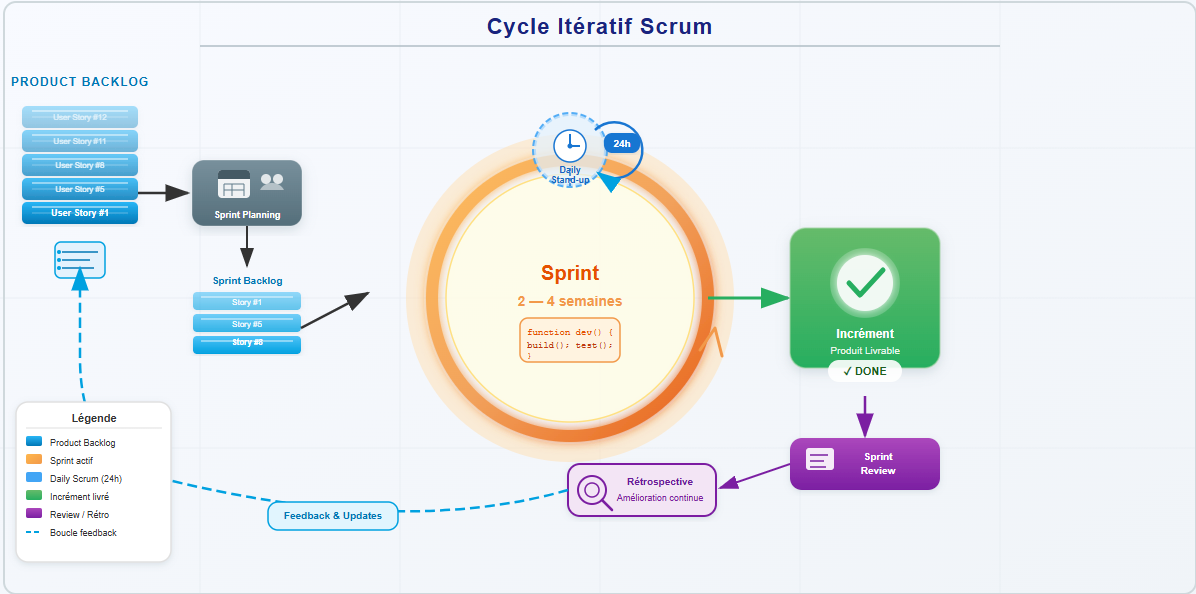
\includegraphics[width=15cm, height=7cm]{Figures/deroulement scrum.png}}
\caption{Déroulement de scrum}\cite{scrum_process_figure}
\label{fig:planification}
\end{figure}

Dans le cadre du développement de SmartRec, la méthodologie Scrum a été mise en œuvre à travers une succession de sprints d'une durée fixe généralement comprise entre deux et quatre semaines, définie dès la phase de cadrage du projet. Cette dernière a permis de clarifier la vision globale de la plateforme, d'établir le backlog initial sous forme de tickets de tâches et de définir le planning général du développement. 

\par Chaque sprint s'est articulé autour de quatre étapes fondamentales :
\begin{itemize}[label=\textbullet]
\item \textbf{La planification du sprint}: en début de chaque sprint, l'équipe se réunissait afin de sélectionner les tickets prioritaires du backlog à traiter et d'identifier les tâches nécessaires à l'atteinte des objectifs fixés, le tout géré et suivi via l'outil \textbf{Trello}.

\item \textbf{Les mêlées quotidiennes (Daily Stand-ups)}: des réunions journalières courtes étaient tenues afin que chaque membre partage l'état d'avancement de ses travaux, ses prévisions et les éventuels obstacles rencontrés, favorisant ainsi une communication fluide et des ajustements rapides.


\item \textbf{La revue du sprint}: à l'issue de chaque sprint, un bilan des livrables produits était dressé afin de vérifier leur conformité aux objectifs initialement définis et d'affiner le backlog pour le sprint suivant.

\item \textbf{La rétrospective du sprint}: cette réunion interne visait à analyser le déroulement du sprint écoulé, à identifier les points positifs à consolider et les axes d'amélioration à exploiter pour optimiser les sprints suivants.


\end{itemize}

\section*{Conclusion} \addcontentsline{toc}{section}{\protect\numberline{}Conclusion}%
\hspace{0.5cm}\textbf
En guise de synthèse, ce chapitre introductif a permis d'établir les fondements conceptuels et méthodologiques du projet \textbf{SmartRec}, en présentant le contexte général et en analysant de manière critique les solutions RH existantes sur le marché. L'identification des lacunes et insuffisances des systèmes actuels a mis en lumière la nécessité de développer une plateforme web innovante, capable d'optimiser et de centraliser la gestion des ressources humaines. Par ailleurs, le recours à la méthodologie agile Scrum a été justifié par sa capacité à allier flexibilité, rigueur organisationnelle et adaptabilité tout au long du cycle de développement. Ce chapitre pose ainsi les jalons indispensables à la bonne conduite et à la réussite du projet dans les phases ultérieures.



%\addcontentsline{toc}{section}{\protect\numberline{}Conclusion}%

\chead{CHAPITRE 2. SPRINT 0 :  ANALYSE ET SPÉCIFICATION DES BESOINS}
 \chapter{Analyse et Spécification des Besoins}
\renewcommand{\mtctitle}{Sommaire}
\minitoc
	\newpage
 \section*{Introduction}
 \addcontentsline{toc}{section}{\protect\numberline{}Introduction}%
Ce chapitre détaille le Sprint 0, phase cruciale d'immersion posant les bases technologiques et fonctionnelles de l'application SmartRec. Il articule l'analyse métier approfondie, la spécification des exigences Salesforce et Heroku, ainsi que la conception de l'architecture cloud intégrée. Sont également exposés le backlog structuré, la modélisation UML des processus de recrutement, la feuille de route Agile et la configuration de l'écosystème de développement SFDX.

\section{Etude du contexte}

L'étude du contexte constitue le pilier de SmartRec, permettant de cartographier l'écosystème de recrutement digital où s'intègre la puissance de Salesforce. Elle définit les attentes précises des recruteurs et candidats, tout en traçant les frontières fonctionnelles entre la gestion des offres et l'automatisation des candidatures. Cette étape assure la viabilité du socle technique, en ancrant chaque cas d'utilisation dans une logique d'optimisation de l'expérience utilisateur et de performance du matching.

\subsection{Identification des acteurs}
Pour appréhender les flux de données et les interactions au sein de SmartRec, il convient de définir précisément les acteurs métiers et leurs périmètres d'action. Le récapitulatif ci-après détaille les privilèges et les responsabilités de chaque profil utilisateur au sein de la plateforme.

 \begin{table}[H]
 \captionsetup{justification=centering}
\caption{Acteurs du système}
\label{tab:acteurs}
\centering
\begin{tabular}{|m{4cm}|m{12cm}|}
\hline 
\centering \textbf{Acteur} & \textbf{Description} \\
\hline Administrateur  & 
Il gère les utilisateurs internes, attribue les rôles, supervise les équipes en désignant les managers, consulte les tâches des employés et accède aux statistiques en temps réel via le tableau de bord.\\
\hline Responsable RH & 
Gère la configuration Salesforce, les habilitations de sécurité, les paramétrages techniques de la plateforme et supervise les tableaux de bord de pilotage global.\\
\hline Recruteur  & 
Pilote le processus de recrutement : création des offres, évaluation des candidatures assistée par les scores de l'IA, gestion des entretiens et sélection des talents.\\
\hline Candidat  &
Utilisateur externe qui postule via le portail dédié, télécharge son CV, gère son profil personnel et suit l’évolution de ses différentes demandes de recrutement.\\
\hline Intelligence Artificielle (NLP)&
Acteur secondaire assurant le parsing automatique des CV (extraction de données) et le calcul du score de matching entre les profils candidats et les offres d'emploi.\\
\hline 
\end{tabular}
\end{table}
\subsection{Spécification des besoins}

La phase de spécification des exigences est capitale pour définir le comportement logique de l'écosystème SmartRec. Elle offre une cartographie précise des fonctionnalités à implémenter sur Salesforce pour garantir une satisfaction optimale des utilisateurs finaux. Cette analyse nous a permis d'organiser les attentes métiers en deux piliers distincts : les besoins fonctionnels et les exigences non fonctionnelles.

\subsubsection{Identification des besoins fonctionnels}
Les besoins fonctionnels détaillent les capacités opérationnelles que SmartRec met à disposition de ses utilisateurs. Ils traduisent les interactions directes que chaque profil peut initier sur la solution Salesforce. Les exigences retenues sont les suivantes :

\hspace{0.5cm}

\begin{itemize}
    \item \textbf{Gestion des accès et des profils utilisateurs :}
    \begin{itemize}
        \item[--]  Les candidats créent leur espace sur le site Experience Cloud pour gérer leur identité et suivre leurs interactions avec l'entreprise.
        \item[--] L'administrateur supervise les comptes des recruteurs, gère les habilitations système et garantit la sécurité des données sur l'organisation Salesforce.
    \end{itemize}
\hspace{0.5cm}

    \item \textbf{Cycle de vie et publication des offres d’emploi:}
\begin{itemize}
    \item[--] Les recruteurs administrent les offres (création, édition, publication) et supervisent leur clôture automatique selon les échéances définies.
     \item[--] Les candidats parcourent l'ensemble des opportunités professionnelles actives publiées sur la plateforme de recrutement.
    \end{itemize} 
\hspace{0.5cm}
    
    \item \textbf{Soumission de candidatures et suivi :}
    \begin{itemize}
        \item[--] Les candidats peuvent postuler aux offres d’emploi via la plateforme.
        \item[--] Ils peuvent suivre le statut de leur candidature (en attente, acceptée ou refusée).
        \item[--] Un système intelligent de tri (scoring automatique) permet de filtrer les candidatures selon leur pertinence.
    \end{itemize}
 \hspace{0.5cm}
    
    \item \textbf{ Dépôt de candidatures et automatisation du tri:}
    \begin{itemize}
        \item[--] Les candidats soumettent leur candidature avec extraction automatique des données de leur CV par l'intelligence artificielle.

        \item[--]Ils visualisent en temps réel l'évolution de leur dossier (À l'étude, Sélectionné ou Refusé) depuis leur espace personnel.

        \item[--] L'IA calcule un score de matching prédictif pour chaque postulant, permettant aux recruteurs de prioriser les profils qualifiés. \end{itemize}

    \end{itemize}
\hspace{0.5cm}

\begin{itemize}
    \item \textbf{GePilotage et supervision de l'activité:}
    \begin{itemize}
        \item[--] Les recruteurs supervisent l'ensemble des candidatures groupées par offre et exploitent les outils de filtrage avancés pour trier les talents.
        \item[--]  L'administrateur surveille la stabilité de la plateforme, les logs système et les statistiques globales de recrutement sur l'organisation.
    \end{itemize}
\hspace{0.5cm}
    
    \item \textbf{Gestion des dossiers et documents:}
    \begin{itemize}
        \item[--] Les recruteurs consultent les dossiers complets des candidats, incluant les CV, les résultats de parsing et les évaluations techniques détaillées.
        \item[--] L'administrateur système garantit l'intégrité des fichiers stockés et gère les autorisations d'accès aux pièces jointes sensibles sur Salesforce.
    \end{itemize}
\hspace{0.5cm}


    \item \textbf{Automatisation et workflow de recrutement:}
    \begin{itemize}
        \item[--] Le système clôture automatiquement les offres dont la date d'échéance est atteinte pour maintenir un catalogue d'opportunités à jour.
        \item[--] Les recruteurs pilotent les étapes du processus, faisant progresser le statut des candidats de l'étude initiale jusqu'à l'embauche finale.
        \item[--]  L'administrateur supervise les processus automatisés pour s'assurer qu'aucun blocage technique n'entrave le flux continu des candidatures.
    \end{itemize}
    
\end{itemize}



\subsubsection{Identification des besoins non fonctionnels}
Afin d'assurer une solution de recrutement robuste, sécurisée et performante sur Salesforce, des exigences non fonctionnelles rigoureuses ont été établies. Elles garantissent la fiabilité technique du système SmartRec et l'optimisation de l'expérience utilisateur.

\hspace{0.5cm}

\begin{itemize}
    \item \textbf{Sécurité et Confidentialité:}
     \begin{itemize}
        \item[--] Protection des données candidats via le modèle de sécurité Salesforce, la gestion fine des profils d'accès et l'authentification Experience Cloud.
    \end{itemize}
\hspace{0.5cm}     

    \item \textbf{Expérience Utilisateur (UX):}
     \begin{itemize}
        \item[--] Interfaces modernes conçues en LWC (Lightning Web Components), offrant une navigation fluide et intuitive pour tous les profils d'utilisateurs.
    \end{itemize}
\hspace{0.5cm}
    \item \textbf{Performance et Réactivité:}
     \begin{itemize}
        \item[--] Optimisation des temps de réponse via l'utilisation du cache client LWC et de traitements asynchrones pour l'analyse des candidatures.
    \end{itemize}
\hspace{0.5cm}
\end{itemize}
\section {Pilotage du projet sous méthodologie SCRUM}
Comme souligné précédemment, la gestion du développement de SmartRec s'appuie sur le framework agile SCRUM. Cette démarche itérative favorise une synergie constante entre les parties prenantes pour livrer une solution Salesforce à haute valeur ajoutée. L'organisation SCRUM retenue s'articule autour de trois piliers fondamentaux :
\vspace{0.3cm}
\begin{table}[H]
\caption{Rôles dans notre projet}
\begin{tabular}{|m{3.5cm}|m{11cm}|}
\hline
\rowcolor{WhiteSmoke} \arrayrulecolor{black}

\hline
\hfil{\cellcolor{WhiteSmoke}\textbf{Role}}
&\hfil{\cellcolor{WhiteSmoke}\textbf{Mission}}\\
 
\hline
\textbf{Product Owner} & Définit la vision produit, priorise le backlog SmartRec et valide l'adéquation des fonctionnalités Salesforce avec les attentes métiers.\\
  \hline

\textbf{Scrum Master} &  Garant du cadre Agile, il lève les obstacles techniques pour assurer la fluidité des sprints et la qualité des livrables de l'application.\\
  \hline
 
\textbf{L’équipe Dev} &  Réalise l'implémentation technique sur Salesforce et Heroku, de la configuration du modèle de données au déploiement des composants LWC.\\
  \hline
\end{tabular}
\end{table}

\section{Backlog produit de SmartRec}

Le Product Backlog constitue le référentiel dynamique des exigences de SmartRec, regroupant les fonctionnalités Salesforce et Heroku à implémenter. Chaque élément — qu'il s'agisse du parsing de CV, du scoring ou de l'interface candidat — est priorisé selon sa valeur métier et sa complexité technique. 
\cite{ScrumOrgBacklog} 
\newline
Il fait office de source de vérité pour l'équipe technique, orientant la planification itérative des sprints de développement. Le Product Owner affine continuellement ces éléments en fonction des retours utilisateurs et des besoins en recrutement, garantissant ainsi un alignement constant avec les objectifs stratégiques du projet.
\cite{AtlassianBacklog} 
\newline
Les principaux attributs de notre backlog:


\begin{itemize}[label=\textbullet]
\item \textbf{ ID } : Identifiant unique permettant la traçabilité de chaque fonctionnalité au sein de l'organisation.
\item \textbf{ User Story} : Expression simplifiée du besoin métier.
\item \textbf{ Priorité } : Niveau d'importance stratégique déterminant l'ordre de traitement dans le flux de développement Agile.
\item \textbf{Sprint} : Itération de travail durant laquelle les fonctionnalités sont conçues, testées et livrées sur l'environnement.\\
\end{itemize}

\begin{table}[H]
\caption{Backlog produit de "SmartRec"}
\centering
\renewcommand{\arraystretch}{1.4}
\begin{tabular}{|p{1.2cm}|p{3.5cm}|p{1.2cm}|p{7.5cm}|p{1.8cm}|}
\hline
\textbf{ID} & \textbf{Fonctionnalit\'e} & \textbf{ID US} & \textbf{User Story} & \textbf{Priorit\'e} \\
\hline

% Administration Salesforce
01 & Administration Salesforce & US 1 & En tant qu'administrateur, je veux configurer les permissions et rôles afin de s'ecuriser les donn'ees RH. & Haute \\
\cline{3-5}
& & US 2 & En tant qu'administrateur, je veux superviser les flux de donn'ees avec le service d'IA (Heroku) pour garantir la stabilit'e. & Haute \\
\cline{3-5}
& & US 3 & En tant qu'utilisateur interne, je veux acc'eder `a des tableaux de bord pour suivre les indicateurs cl'es du recrutement. & Haute \\
\hline

% Espace Candidat
02 & Espace Candidat & US 4 & En tant que candidat, je veux cr'eer un compte sur Experience Cloud pour acc'eder au portail de recrutement. & Haute \\
\cline{3-5}
& & US 5 & En tant que candidat, je veux g'erer mon profil professionnel via l'interface LWC. & Haute \\
\hline

% IA
03 & Analyse de Candidatures & US 6 & En tant que candidat, je veux postuler en t'el'echargeant mon CV pour une extraction automatique de mes donn'ees (Parsing). & Haute \\
\cline{3-5}
& & US 7 & En tant que recruteur, je veux visualiser pour chaque candidat un score de matching calcul'e par l'IA. & Haute \\
\hline

% Gestion du Cycle des Offres
04 & Cycle des Offres & US 8 & En tant que recruteur, je veux publier et modifier des offres d'emploi directement depuis l'organisation. & Haute \\
\cline{3-5}
& & US 9 & En tant que syst`eme, je veux clôturer automatiquement les offres dont la date d''ech'eance est d'epass'ee. & Moyenne \\
\cline{3-5}
& & US 10 & En tant que candidat, je veux consulter et filtrer les opportunit'es professionnelles disponibles en ligne. & Moyenne \\

\hline
\end{tabular}
\end{table}


\begin{table}[H]
\centering
\renewcommand{\arraystretch}{1.4}
\begin{tabular}{|p{1.2cm}|p{3cm}|p{1.2cm}|p{8cm}|p{1.8cm}|}
\hline

% Suivi & Gestion
05 & Suivi et Gestion & US 11 & En tant que candidat, je veux suivre en temps r'eel l''etat d'avancement de mes candidatures. & Moyenne \\
\cline{3-5}
& & US 12 & En tant que recruteur, je veux g'erer les dossiers candidats et consulter les CV via une interface centralis'ee. & Moyenne \\
\hline

% Recrutement intelligent & ATS
06 & Recrutement intelligent & US 13 & En tant que recruteur, je veux utiliser le moteur de matching pour filtrer automatiquement les candidats les plus pertinents. & Moyenne \\
\cline{3-5}
& & US 14 & En tant que recruteur, je veux changer le statut d'une candidature afin de faire progresser le dossier dans le workflow. & Moyenne \\
\cline{3-5}
& & US 15 & En tant que recruteur, je veux acc'eder aux informations d'etaill'ees extraites du CV par l'IA pour 'evaluer le profil. & Moyenne \\
\cline{3-5}
& & US 16 & En tant que recruteur, je veux effectuer des actions group'ees sur les candidatures pour optimiser le traitement des dossiers. & Moyenne \\
\hline

% Gestion des viviers et rapports
07 & Gestion des projets & US 17 & En tant que recruteur, je veux cr'eer des dossiers de talents afin de classer les candidats par type de profil. & Moyenne \\
\cline{3-5}
& & US 18 & En tant qu'administrateur, je veux configurer les crit`eres de matching par d'efaut pour l'intelligence artificielle. & Moyenne \\
\cline{3-5}
& & US 19 & En tant que recruteur, je veux partager une candidature avec d'autres coll`egues pour avis collaboratif. & Moyenne \\
\cline{3-5}
& & US 20 & En tant que recruteur, je veux acc'eder `a l'historique complet des interactions avec un candidat. & Moyenne \\
\cline{3-5}
& & US 21 & En tant qu'administrateur, je veux g'erer les mod`eles d'e-mails automatiques envoy'es aux candidats. & Moyenne \\
\cline{3-5}
& & US 22 & En tant que recruteur, je veux consulter les statistiques de performance des offres publi'ees. & Moyenne \\
\hline

\end{tabular}
\end{table}

\begin{table}[H]
\centering
\renewcommand{\arraystretch}{1.4}
\begin{tabular}{|p{1.2cm}|p{3cm}|p{1.2cm}|p{8cm}|p{1.8cm}|}
\hline

% Expérience Utilisateur & Sécurité
08 & Sécurité et Support & US 23 & En tant que candidat, je veux acc'eder `a une section d'aide afin de comprendre le processus de recrutement. & Basse \\
\cline{3-5}
& & US 24 & En tant que recruteur, je veux archiver les anciennes offres afin de nettoyer la vue op'erationnelle. & Basse \\
\cline{3-5}
& & US 25 &  En tant qu'administrateur, je veux configurer les param`etres de confidentialit'e des donn'ees (RGPD). & Basse \\
\hline

% Maintenance & Personnalisation
09 & Personnalisation  & US 26 & En tant que candidat, je veux r'ecup'erer mon mot de passe en cas d'oubli via une proc'edure automatis'ee. & Basse \\
\cline{3-5}
& & US 27 & En tant que recruteur, je veux personnaliser l'affichage de ma liste de candidatures selon mes pr'ef'erences. & Basse \\
\cline{3-5}
& & US 28 & En tant qu'administrateur, je veux pouvoir activer ou d'esactiver les services d'IA (Parsing/Scoring) & Basse \\
\cline{3-5}
& & US 29 & En tant que recruteur, je veux exporter les donn'ees des candidats retenus pour des besoins de reporting. & Basse \\
\hline

\end{tabular}
\end{table}


\section{Modélisation fonctionnelle : Diagramme de cas d’utilisation generale} 
Le diagramme de cas d'utilisation synthétise les interactions entre les candidats, les recruteurs et l'administrateur avec le cœur de l'application SmartRec. Il expose les fonctionnalités majeures — du parsing de CV au matching intelligent — tout en délimitant les responsabilités et les flux opérationnels de chaque acteur.

\begin{figure}[H]
\centering
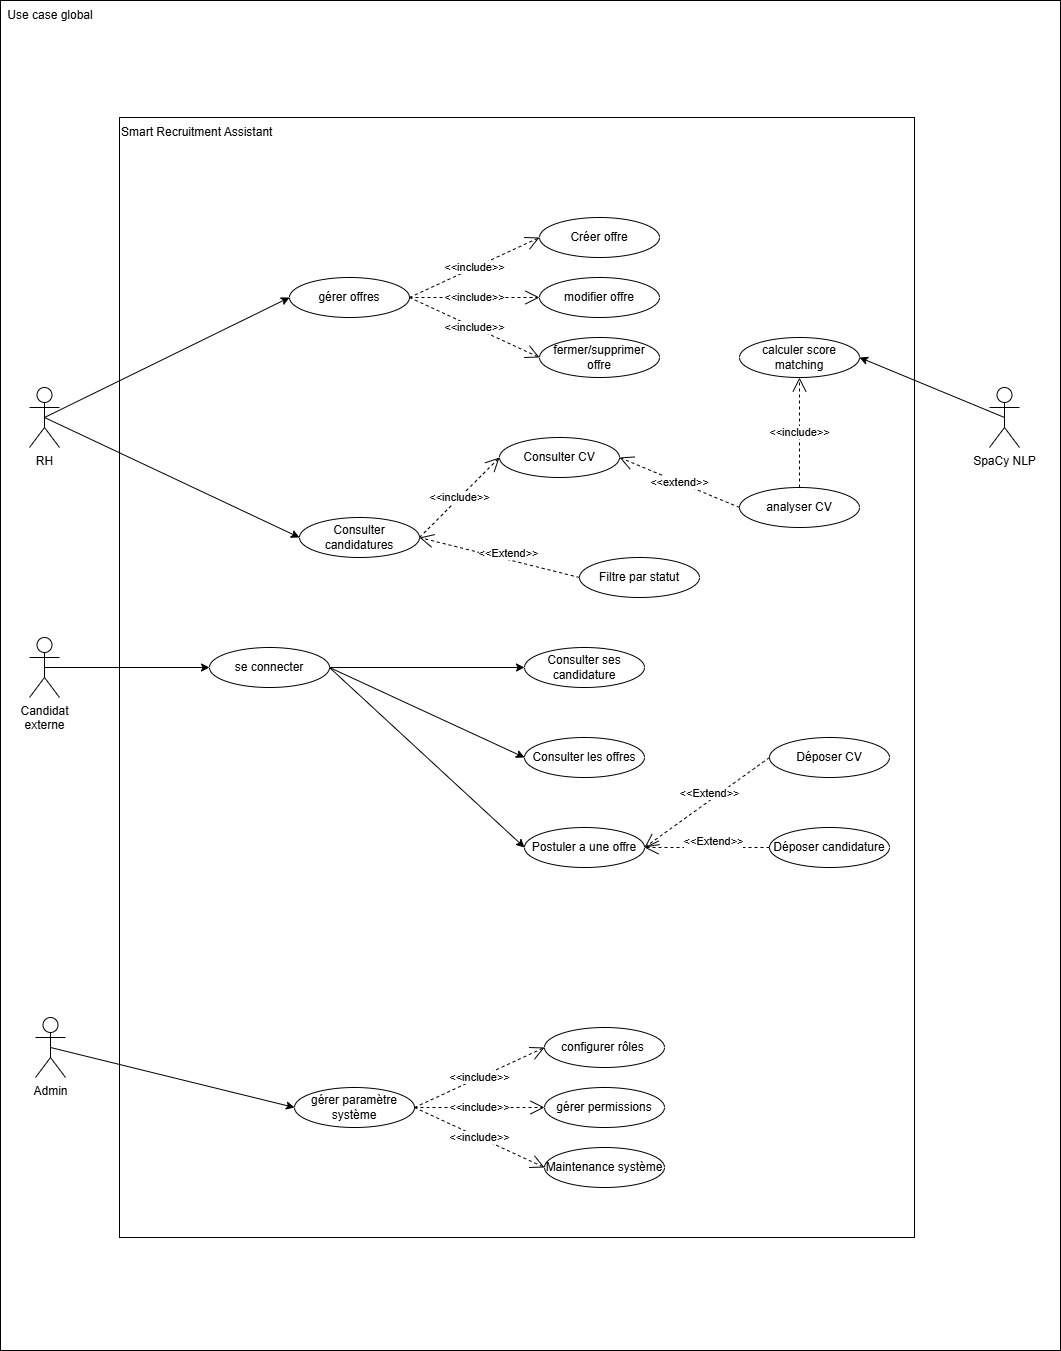
\includegraphics[width=19cm, height=20cm]{Figures/USE case globale.png}
\caption{Diagramme de cas d’utilisation global}
\label{schema1}
\end{figure}
 




\newpage
\section{Conception de la base de données : Diagramme de classes}
Le diagramme de classes structure la modélisation de données de SmartRec, définissant les objets Salesforce (Offre, Candidature, Person Account), 
leurs attributs métiers et les relations d'association. Cette étape est déterminante pour garantir la cohérence du schéma de données et 
l'efficacité des traitements automatisés par les triggers et batchs Apex.

\begin{figure}[H]
\centering

\includegraphics[width=18cm, height=16cm]{Figures/diagramme de classe globale.png'}
\caption{Diagramme de classe global}
\label{schema1}
\end{figure}


\newpage





\section{Feuille de route Agile : Planification des sprints }
Pour garantir une livraison itérative de valeur, le développement de SmartRec a été structuré en 5 sprints distincts. 
Cette organisation repose sur la priorisation du backlog produit, assurant que les socles techniques essentiels précèdent les fonctionnalités de surface.

La réalisation s'est étalée sur une durée de cinq mois, du 2 février au 30 juin 2026. 
Le mois initial a été dédié à l'immersion métier, l'analyse du contexte et la conception technique de l'écosystème Salesforce. 
Le tableau suivant synthétise le cadencement des développements et les objectifs associés à chaque itération.

\vspace{0.3cm}
\begin{table}[H]
\caption{Planification des sprints}
\begin{tabular}{|m{2cm}|m{2.5cm}|m{5cm}|m{6cm}|}
\hline
\rowcolor{WhiteSmoke} \arrayrulecolor{black}

\hfil{\cellcolor{WhiteSmoke}\textbf{Sprint}} &
\hfil{\cellcolor{WhiteSmoke}\textbf{Durée}} &
\hfil{\cellcolor{WhiteSmoke}\textbf{User Stories inclues}} &
\hfil{\cellcolor{WhiteSmoke}\textbf{Objectif du sprint}} \\
\hline

\textbf{Sprint 1} & 4 semaines &
US1, à US5 &
Mise en place de l'organisation Salesforce, gestion des profils/permissions et portail candidat Experience Cloud. \\
\hline

\textbf{Sprint 2} & 4 semaines &
US6, à US8 &
Gestion du cycle de vie des offres d'emploi, publication en ligne et automatisation de la clôture des offres. \\
\hline

\textbf{Sprint 3} & 4 semaines &
US 9 à US 10&
Intégration de l'intelligence artificielle pour le parsing automatique des CV et calcul des scores de matching. \\
\hline

\textbf{Sprint 4} & 4 semaines &
US 11 à US 16  &
Développement du workflow ATS, suivi des candidatures et interface de gestion intelligente pour les recruteurs. \\
\hline

\textbf{Sprint 5} & 4 semaines &
US 17 à US 29   &
Gestion des viviers de talents, tableaux de bord de pilotage, sécurisation RGPD et personnalisation de l'expérience. \\
\hline

\end{tabular}
\end{table}



 \section{ Environnement de développement }
 \hspace{0.5cm}\textbf Le choix d'un écosystème d'outils performants est une étape déterminante pour la réussite du projet SmartRec. Cette section présente l'environnement matériel et les solutions logicielles mobilisés pour la conception et la réalisation de la plateforme.


 
\subsection{Environnement matériel}
Pour assurer la fluidité du développement et la stabilité des outils de build Salesforce, les ressources suivantes ont été utilisées :

\begin{itemize}[label=\textbullet]
\item Ordinateur : Laptop Lenovo haute performance.
\item Processeur : Intel Core Ultra 7, optimisé pour les tâches de compilation.
\item Mémoire vive : 32 Go de RAM pour supporter l'exécution simultanée des IDE et navigateurs. 
\item Système d'exploitation : Windows 11 Famille (Version Unilingue).
\end{itemize}


\subsubsection{Outil de rédaction du rapport}
\hspace{0.5cm}

Le rapport a été rédigé avec \textbf{Overleaf}, un éditeur en ligne basé sur LaTeX, qui permet d’écrire à plusieurs tout en visualisant instantanément le rendu.
Cette plateforme est issue de la fusion entre Overleaf et ShareLaTeX en 2017, donnant naissance à une version améliorée : Overleaf v2., offrant une expérience plus complète et optimisée.
\begin{figure}[H]
\centering

\includegraphics[width=2cm]{ Figures/overleaf-logo.jpg}
\caption{Logo du "LaTeX"}\cite{overleaf_logo}
\end{figure}
\subsubsection{Environnement de développement logiciel}
\hspace{0.5cm}
Pour la réalisation de SmartRec, nous avons exploité l'écosystème Salesforce, complété par des outils de développement modernes assurant agilité et robustesse technique.

\begin{itemize}[label=\textbullet]
\item \textbf{ Salesforce Platform et Apex } :  L'infrastructure cloud fournissant la base de données et 
le langage backend Apex. Ce dernier permet de gérer la logique métier complexe (triggers, batchs) 
de l'application.
\begin{figure}[H]
\centering
\includegraphics[width=2cm]{ Figures/Salesforce_logo.png}
\caption{Logo du  "Salesforce"}\cite{Salesforce_logo}
\end{figure}
\item \textbf{ Lightning Web Components (LWC)} : Le framework UI moderne de Salesforce utilisé pour 
concevoir les interfaces réactives et dynamiques du portail candidat et des outils recruteurs.
\begin{figure}[H]
\centering

\includegraphics[width=2cm]{ Figures/LWC_logo.png}
\caption{Logo du"LWC"}\cite{LWC-logo}
\end{figure}
\item \textbf{ Experience Cloud } : Solution utilisée pour bâtir le site de recrutement externe, permettant aux candidats d'interagir de manière sécurisée avec le système SmartRec. 
\begin{figure}[H]
\centering

\includegraphics[width=2cm]{ Figures/experiencecloud_logo.png}
\caption{Logo du "Experience Cloud"}\cite{experiencecloud_logo}
\end{figure}
\item \textbf{Visual Studio Code} :  Éditeur de code principal, enrichi du "Salesforce Extension Pack". 
Il a permis le développement des composants, l'écriture du code Apex et la gestion des déploiements.
\begin{figure}[H]
\centering

\includegraphics[width=2cm]{ Figures/vs.jpg}
\caption{Logo du "Visual Studio"}\cite{vscode_logo}
\end{figure}
\item \textbf{Salesforce CLI (SFDX) } : Outil en ligne de commande indispensable pour automatiser les déploiements, gérer les environnements et synchroniser le code source avec l'organisation.
\begin{figure}[H]
\centering

\includegraphics[width=2cm]{ Figures/SalesforceCli.png}
\caption{Logo du "Salesforce CLI"}\cite{SalesforceCli}
\end{figure}
\item \textbf{GitHub } : Plateforme de gestion de version utilisée pour centraliser le code source, assurer le suivi des modifications et sécuriser l'historique du développement.
\begin{figure}[H]
\centering
\includegraphics[width=2cm]{ Figures/GitHub_logo.png}
\caption{Logo du "GitHub"}\cite{GitHub-logo}
\end{figure}
\item \textbf{Python } : Utilisé pour développer le moteur d'intelligence artificielle (NLP) hébergé sur Heroku. Il assure le traitement automatique du langage naturel pour extraire les compétences et expériences des fichiers PDF.
\begin{figure}[H]
\centering

\includegraphics[width=2cm]{ Figures/Python-logo.png}
\caption{Logo du "Python"}\cite{python_logo}
\end{figure}
\item \textbf{Apidog } :  Outil utilisé pour tester et documenter les API REST reliant Salesforce au service de parsing. Il a permis de valider la communication et le format des données JSON échangées.
\begin{figure}[H]
\centering

\includegraphics[width=2cm]{ Figures/apidog-logo.png}
\caption{Logo du "Apidog"}\cite{apidog_logo}
\end{figure}
\item \textbf{Draw.io } :  Utilisé pour concevoir les différents diagrammes du projet (classes, cas d’utilisation, architecture), permettant une modélisation claire du système SmartRec.
\begin{figure}[H]
\centering

\includegraphics[width=2cm]{ Figures/draw-logo.png}
\caption{Logo du "Draw.io"}\cite{drawio_logo}
\end{figure}
\end{itemize}



\section{Architecture du système}
\hspace{0.5cm}
La conception architecturale de SmartRec a été pensée pour allier la puissance de la plateforme Salesforce à la flexibilité des services d'IA. Elle définit l'organisation des composants logiciels et leurs protocoles de communication, garantissant ainsi une structure évolutive et sécurisée.

\subsection{Architecture globale de la solution}
\hspace{0.5cm}
 L'architecture de SmartRec repose sur un modèle hybride Cloud-to-Cloud, séparant le portail candidat (Experience Cloud), la gestion métier (Salesforce Core) et le moteur de parsing (Heroku / Python). Cette approche modulaire permet de découpler l'interface utilisateur de la complexité algorithmique du traitement automatique du langage naturel (NLP).

 \begin{itemize}
    \item Une interface utilisateur développée avec les \textbf{Lightning Web Components (LWC)}, sur le portail \textbf{Experience Cloud} pour offrir une expérience fluide et moderne aux candidats.

    \item Un back-end robuste conçu avec le langage \textbf{Apex} au sein de la plateforme Salesforce pour orchestrer la logique métier complexe et les processus automatisés.
    
    \item Une base de données intégrée basée sur les \textbf{Objets Salesforce} (standards et personnalisés), utilisée pour stocker de manière sécurisée les offres, candidatures et profils.

    \item Un microservice indépendant en \textbf{Python}, hébergé sur \textbf{Heroku}, dédié au traitement intelligent (NLP) des CV et au calcul des scores de matching sémantique.
    
\end{itemize}


\hspace{0.5cm}
\begin{itemize}[label=\textbullet]
\item L'interopérabilité entre ces modules est assurée par des API REST sécurisées, garantissant une séparation stricte des responsabilités et une maintenance simplifiée de la solution.

\begin{figure}[H]
\centering
\fbox{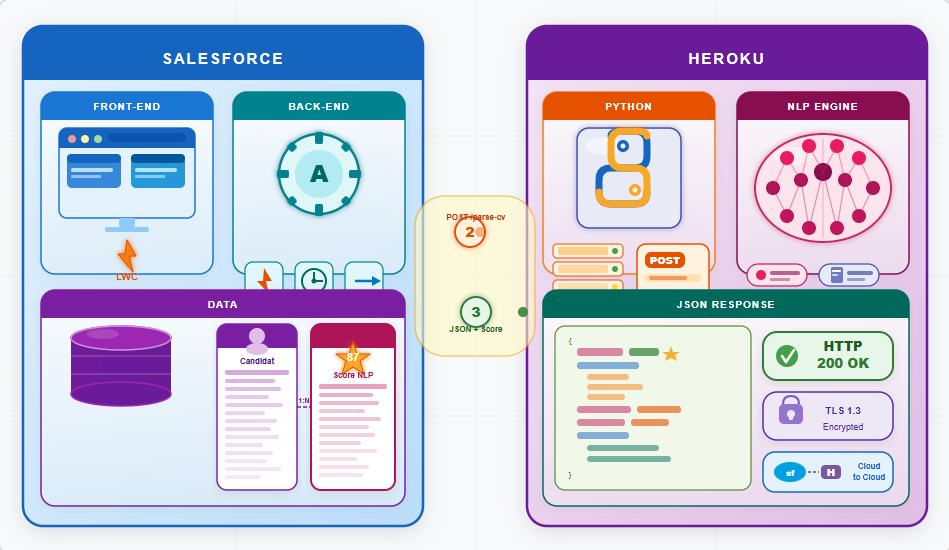
\includegraphics[width=15cm, height=7cm]{Figures/architecture physique.png}}
\caption{Architecture globale}\cite{munonye_microservices_2021}
\label{fig:planification}
\end{figure}



\subsection{Architecture physique}
L’architecture physique décrit la répartition des composants de SmartRec sur les infrastructures cloud et matérielles. Elle illustre la nature distribuée de la solution, garantissant sécurité et scalabilité.

\hspace{0.2cm}
Dans le cadre du projet, l'organisation est la suivante:
\begin{itemize}[label=\textbullet]
\item \textbf{Poste de développement (Local):}Utilisé pour la rédaction du code source (VS Code) et le contrôle de version (Git/GitHub).
\item \textbf{Cloud Salesforce (PaaS) :}Héberge l'interface utilisateur (Experience Cloud), la logique métier (Apex) et le stockage des données (Objets Salesforce).
\item \textbf{Cloud Heroku (PaaS) : }Héberge le microservice Python dédié au traitement NLP des CV, isolant ainsi les tâches de calcul intensif.
\end{itemize}
Les communications entre ces entités s'appuient sur le protocole HTTPS, assurant une transmission cryptée et sécurisée des données sur le réseau internet.
\end{itemize}

\begin{figure}[H]
\centering
\fbox{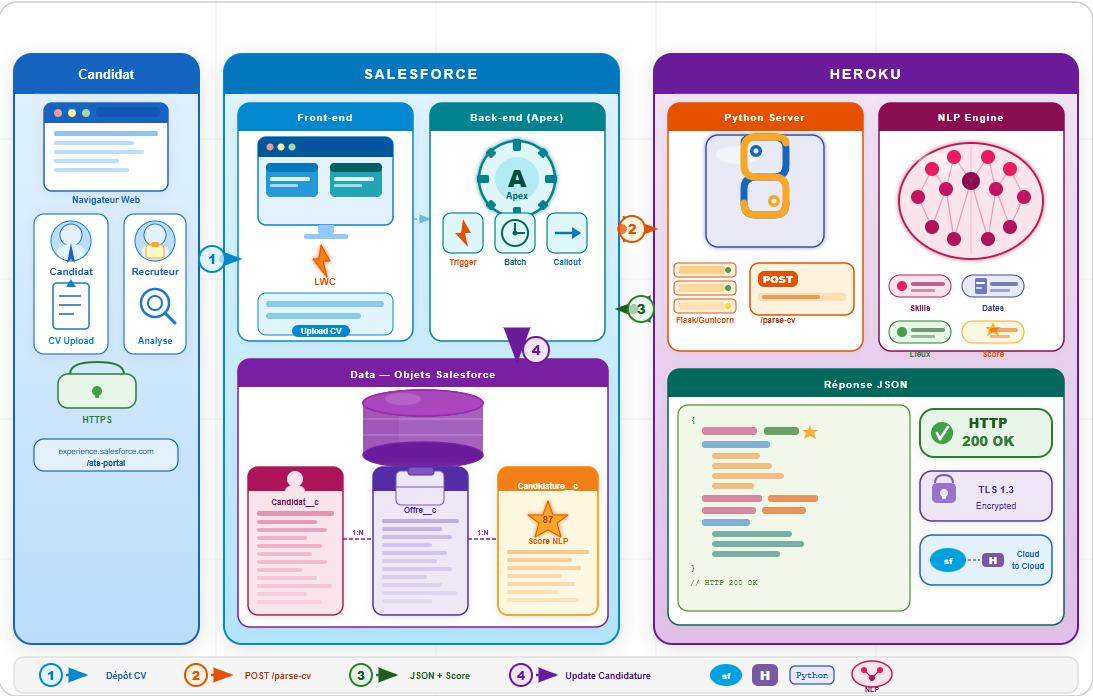
\includegraphics[width=15cm, height=7cm]{Figures/architecture globale.png}}
\caption{Architecture physique}\cite{homedeve_architecture_physique_2023}
\label{fig:planification}
\end{figure}

\subsection{Architecture logique }  
L'architecture logique de SmartRec repose sur le paradigme MVC (Modèle-Vue-Contrôleur), nativement supporté par Salesforce. Cette structure garantit une séparation nette des responsabilités, facilitant la maintenance et l'évolutivité de la solution.
L'application s'articule autour des couches suivantes :
\begin{itemize}[label=\textbullet]
\item \textbf{La Vue (LWC) :}Gère l'interface utilisateur et les interactions dynamiques sur le portail Experience Cloud. 
\item \textbf{Le Contrôleur (Apex) : }Assure la médiation entre l'interface et la base de données, traitant les requêtes envoyées par les composants LWC.
\item \textbf{Le Modèle (Objets Salesforce) :}Définit la structure des données (Offres, Candidatures, Contacts) et assure leur persistance sécurisée.
\item \textbf{La Couche Logique (Triggers et Classes Services) :}Gère les automatisations métier, comme le scoring IA ou les règles de validation anti-doublon.
\end{itemize}
Cette modularité permet de dissocier les traitements complexes de l'interface graphique, assurant ainsi une performance optimale et des tests unitaires simplifiés.

\begin{figure}[H]
\centering
\fbox{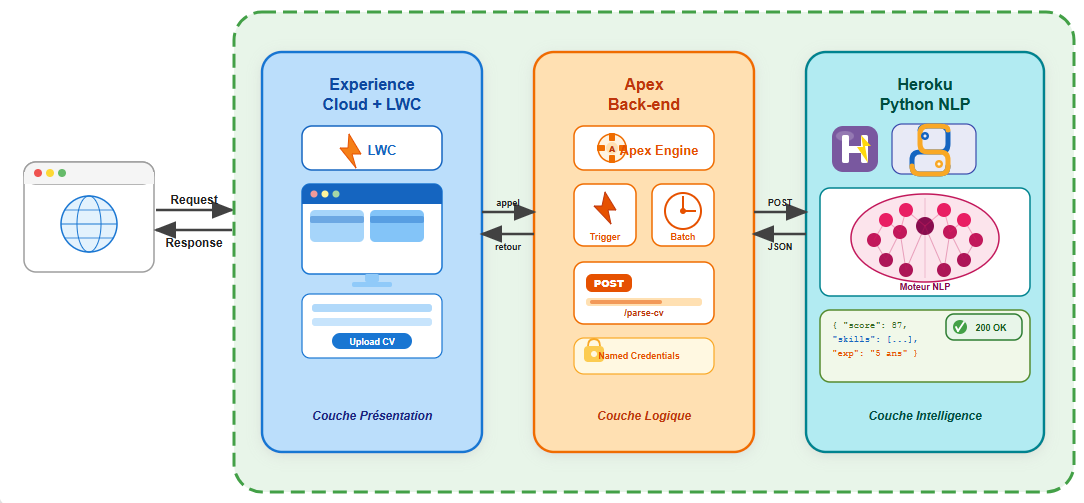
\includegraphics[width=15cm, height=7cm]{Figures/architecture logique.png}}
\caption{Architecture logique}\cite{dyma_springboot_2023}
\label{fig:planification}
\end{figure}

\section*{Conclusion}
Ce chapitre a permis de poser les jalons méthodologiques et techniques indispensables à la réalisation de SmartRec. Nous avons traduit les besoins métiers en spécifications fonctionnelles via le backlog produit et les cas d'utilisation, avant de concevoir une architecture hybride (Salesforce et Heroku) répondant aux exigences de scalabilité. Enfin, la planification détaillée des sprints a été établie pour structurer la phase de développement. Le chapitre suivant sera consacré au premier sprint, dédié à la mise en place du socle de sécurité et à la gestion des accès utilisateurs. 
\addcontentsline{toc}{section}{\protect\numberline{}Conclusion}%

\chead{CHAPITRE 3. SPRINT 1 : Authentification & Gestion des Identités}

\chapter{Sprint 1: Authentification et Gestion des Identités}
\renewcommand{\mtctitle}{Sommaire}
\minitoc
	\newpage

\section*{Introduction}
\addcontentsline{toc}{section}{\protect\numberline{}Introduction}
Le coup d'envoi technique de \textbf{SmartRec} se concrétise à travers ce premier sprint, dont la vocation première est de sécuriser l'accès à la plateforme et de structurer l'écosystème utilisateur. Dans les pages qui suivent, nous explorerons comment l'architecture Salesforce a été exploitée pour bâtir un système d'authentification robuste. Nous détaillerons le passage du backlog fonctionnel à la mise en œuvre concrète des portails recruteurs et candidats, en illustrant chaque avancée par des visuels issus de l'environnement de production.

\section{Objectifs du Sprint}
L’enjeu majeur de cette itération initiale réside dans la segmentation fine des accès. Il s'agit non seulement de permettre une connexion sécurisée, mais surtout de garantir que chaque acteur — qu'il s'agisse d'un administrateur PwC ou d'un candidat externe — interagisse avec une interface adaptée à ses prérogatives métier, grâce à la flexibilité d'Experience Cloud.


\section{Spécification des besoins}
\par Dans cette section, nous présentons le diagramme des cas d’utilisation du sprint ainsi que le backlog associé. L'objectif est de définir clairement les interactions entre les utilisateurs (Administrateur, Recruteur et Candidat) et la plateforme Salesforce.
\subsection{Diagramme cas d’utilisation du Sprint 1}

 \begin{figure}[H]
    \centering
    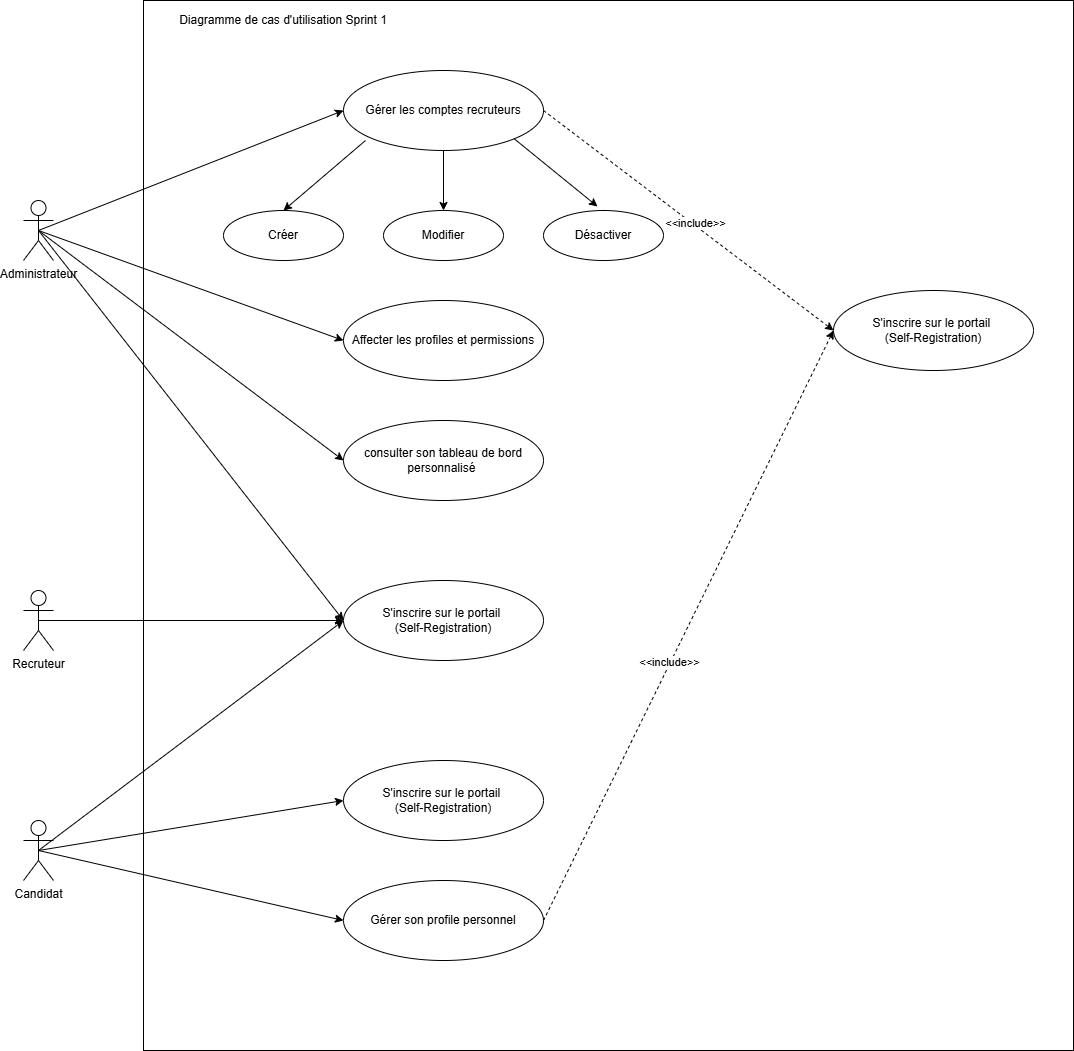
\includegraphics[width=12cm, height=12cm]{Figures/use case 1.png}
    \caption{Diagramme de cas d’utilisation du sprint 1}
    \label{fig:Diagramme de cas d’utilisation du sprint 0}
\end{figure}


\subsection{ Sprint Backlog du sprint 1}
Le tableau ci-dessous présente le sprint backlog établi pour le premier sprint. Il récapitule les différentes user stories sélectionnées, accompagnées de leurs identifiants uniques, ainsi que les tâches techniques à réaliser pour chacune. Ce tableau permet d’avoir une vision claire et structurée du travail prévu, en facilitant la planification, la répartition des responsabilités et le suivi de l’avancement tout au long du sprint.
\begin{table}[H]
\caption{Backlog du sprint 1 : Gestion des utilisateurs et accès}
    \centering
    \begin{tabular}{|p{1cm}|p{8cm}|p{8cm}|}
    \hline
    \textbf{ID} & \textbf{User Story} & \textbf{Tâches techniques (Salesforce)} \\
    \hline
    US-1 & En tant qu'administrateur, je veux créer les comptes des recruteurs afin de leur donner accès au CRM.
    & 
    \begin{itemize}[leftmargin=*]
    \item Configuration des profils et rôles Salesforce.
    \item Création de l'objet utilisateur interne.
    \item Attribution des Permission Sets.
    \end{itemize} \\
    \hline
    US-2 & En tant qu'administrateur, je veux gérer (modifier/désactiver) les comptes utilisateurs. & 
    \begin{itemize}[leftmargin=*]
    \item Configuration des Layouts de page utilisateur.
    \item Mise en place de flux d'automatisation (Flows).
    \end{itemize} \\
    \hline
    US-3 & En tant qu'administrateur, je veux consulter la liste complète des utilisateurs internes pour superviser les accès.  & 
    \begin{itemize}[leftmargin=*]
    \item Configuration des vues de liste personnalisées.
    \item Mise en place de filtres par profil (Recruteur Platform).
    \end{itemize} \\
    \hline
    US-4 & En tant qu'utilisateur, je veux accéder à un tableau de bord Salesforce pour visualiser mes indicateurs clés.& 
    \begin{itemize}[leftmargin=*]
    \item Création de rapports et tableaux de bord natifs.
    \item Personnalisation de la page d'accueil Lightning.
    \end{itemize} \\
    \hline
    US-6 & En tant que candidat, je veux créer un compte sur le portail pour postuler aux offres.& 
    \begin{itemize}[leftmargin=*]
    \item Activation du portail Experience Cloud.
    \item Configuration du "Self-Registration" (inscription libre).
    \item Mapping automatique Candidat/Contact.
    \end{itemize} \\
    \hline
    US-7 & En tant que candidat, je veux mettre à jour mon profil et mes informations personnelles.& 
    \begin{itemize}[leftmargin=*]
    \item Développement d'un formulaire LWC pour l'objet Contact/Candidat.
    \item Gestion de la persistance des données via Apex DML.
    \end{itemize} \\
    \hline
    \end{tabular}
    \label{tab:user_stories_sprint1}
\end{table}

\section{Analyse des besoins}
Avant de traduire les exigences fonctionnelles en modèles techniques, il est primordial de décortiquer les parcours utilisateurs identifiés dans le backlog. Cette étape d'analyse textuelle permet de clarifier les règles de gestion et les comportements attendus du système Salesforce face aux sollicitations des acteurs.

\subsection{Description détaillée des cas d'utilisation}
        \begin{itemize}
        \item \textbf{Cas d'utilisation "Gérer les comptes recruteurs" :} La table 3.2 formalise le processus d'administration des utilisateurs internes au sein de l'organisation.
    \end{itemize}
    \begin{table}[H]
    \caption{Description textuelle du cas d'utilisation "Gérer les comptes recruteurs"}
    \centering
    \begin{tabular}{|c|p{12cm}|}
    \hline
    \textbf{Titre} & Gérer les comptes recruteurs \\
    \hline
    \textbf{Objectif} & Octroyer, modifier ou révoquer l'accès aux modules de recrutement pour les collaborateurs PwC. \\
    \hline
    \textbf{Acteur}& Administrateur\\
    \hline
    \textbf{Pré-condition} & Session administrateur active avec privilèges de gestion des utilisateurs. \\
    \hline
    \textbf{Post-condition} & Les privilèges d'accès sont immédiatement mis à jour dans l'annuaire Salesforce. \\
    \hline
    \textbf{Scénario nominal} & 1. L'administrateur se rend dans l'espace de gestion des utilisateurs. \newline
    2. Il définit le type d'utilisateur et saisit ses informations d'identité. \newline
    3. Il valide les paramètres de sécurité. \newline
    4. Le système déclenche l'envoi d'un e-mail d'activation au nouvel utilisateur. \\
    \hline
    \end{tabular}
    \label{tab:uc_accounts}
\end{table}




\begin{itemize}
        \item \textbf{Cas d'utilisation "Gérer les permissions et profils" :} La table 3.3 présente la description textuelle du cas d'utilisation relatif à la gestion des droits d'accès.
    \end{itemize}
    \begin{table}[H]
    \caption{Description textuelle du cas d’utilisation "Gérer les permissions"}
    \centering
    \begin{tabular}{|c|p{12cm}|}
    \hline
    \textbf{Titre} & Gérer les permissions et profils \\
    \hline
    \textbf{Objectif} & Permettre à l’administrateur d’attribuer des profils et Permission Sets spécifiques aux recruteurs. \\
    \hline
    \textbf{Acteur}& Administrateur\\
    \hline
    \textbf{Pré-condition} & L'utilisateur doit exister dans l'organisation Salesforce. \\
    \hline
    \textbf{Post-condition} & L'utilisateur dispose des accès restreints selon son rôle métier.\\
    \hline
    \textbf{Scénario nominal} & 1. L’administrateur accède à la configuration (Setup) de Salesforce. \newline
    2. Il recherche l'utilisateur cible. \newline
    3. Il sélectionne le profil adéquat (ex: Recruteur Standard). \newline
    4. Il affecte les ensembles de permissions (Permission Sets) nécessaires. \\
    \hline
    \end{tabular}
    \label{tab:uc_permissions}
\end{table}
\begin{itemize}
        \item \textbf{Cas d'utilisation "Consulter le tableau de bord" :} La table 3.4 décrit l'accès aux indicateurs de recrutement.
    \end{itemize}
    \begin{table}[H]
    \caption{Description textuelle du cas d’utilisation "Consulter le tableau de bord"}
    \centering
    \begin{tabular}{|c|p{12cm}|}
    \hline
    \textbf{Titre} & Consulter le tableau de bord de recrutement \\
    \hline
    \textbf{Objectif} & Permettre au recruteur de visualiser les statistiques clés (offres actives, candidatures reçues). \\
    \hline
    \textbf{Acteur}& Recruteur \\
    \hline
    \textbf{Pré-condition} & Le recruteur doit être authentifié sur l'application Salesforce. \\
    \hline
    \textbf{Post-condition} & Les rapports et graphiques de performance sont affichés en temps réel.\\
    \hline
    \textbf{Scénario nominal} & 1. Le recruteur accède à la page d'accueil de SmartRec. \newline
    2. Le système charge les composants LWC de statistiques. \newline
    3. Le recruteur visualise le nombre total de candidatures et leur répartition par statut. \\
    \hline
    \end{tabular}
    \label{tab:uc_dashboard}
\end{table}






\section{Conception}
\hspace{0.5cm}\textbf{Cette section détaille la phase de conception technique propre aux fonctionnalités du premier sprint. En nous appuyant sur le diagramme de classes global présenté au chapitre précédent (Chapitre 2, Figure 2.X), nous nous focalisons ici sur la modélisation dynamique. À travers des diagrammes de séquences, nous illustrons les interactions fluides entre les composants LWC, les contrôleurs Apex et les objets standards de Salesforce (User, Contact, Profile) mis en œuvre lors de l'inscription et de la gestion des identités.}








\subsection{Modélisation de la dynamique (Diagrammes de séquences)}
Pour illustrer la cinématique des échanges entre les différents composants du système, nous avons élaboré des diagrammes de séquences. Ces derniers mettent en lumière la collaboration entre les interfaces LWC, les contrôleurs Apex et la base de données. Le scénario ci-dessous se concentre sur l'un des flux les plus critiques du Sprint 1 : la création autonome d'un compte candidat.

\subsubsection{Diagramme de séquence : Création d'un compte candidat}
Cette vue détaille la chronologie des messages et des traitements lors de l'inscription d'un nouvel utilisateur sur le portail Experience Cloud.


\begin{figure}[H]
\centering
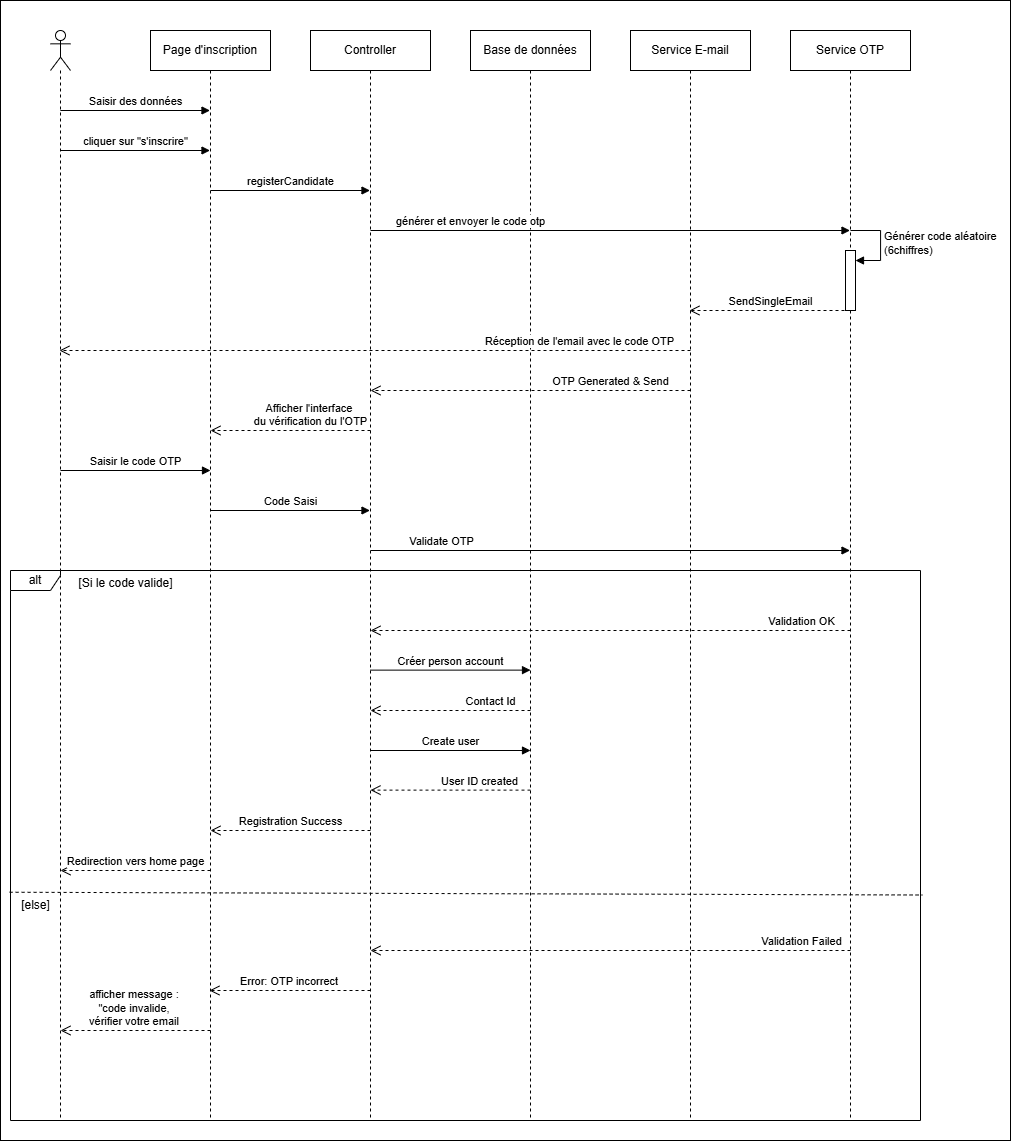
\includegraphics[width=18cm, height=19cm]{Figures/seq1.png}
\caption{Diagramme de séquence ”Créer un compte”}
\label{schema1}
\end{figure}
 




\section{Réalisation : interfaces utilisateur sur Salesforce}
Dans le cadre de ce sprint, les interfaces ont été réalisées en s'appuyant sur les standards de la plateforme Salesforce (Lightning Design System - SLDS). Cette section présente les vues principales de SmartRec, incluant les consoles d'administration et le portail Experience Cloud dédié aux candidats.


\vspace{5mm}
\begin{itemize}
    \begin{itemize}
         \item \textbf{Tableau de bord Recruteur (Lightning Experience) :} Le tableau de bord offre une vue d’ensemble en temps réel sur les indicateurs clés du recrutement : nombre d'offres actives, total de candidatures reçues et répartition des candidats par étape du processus. Il s'appuie sur les composants graphiques natifs de Salesforce.
         \begin{figure}[H]
             \centering
             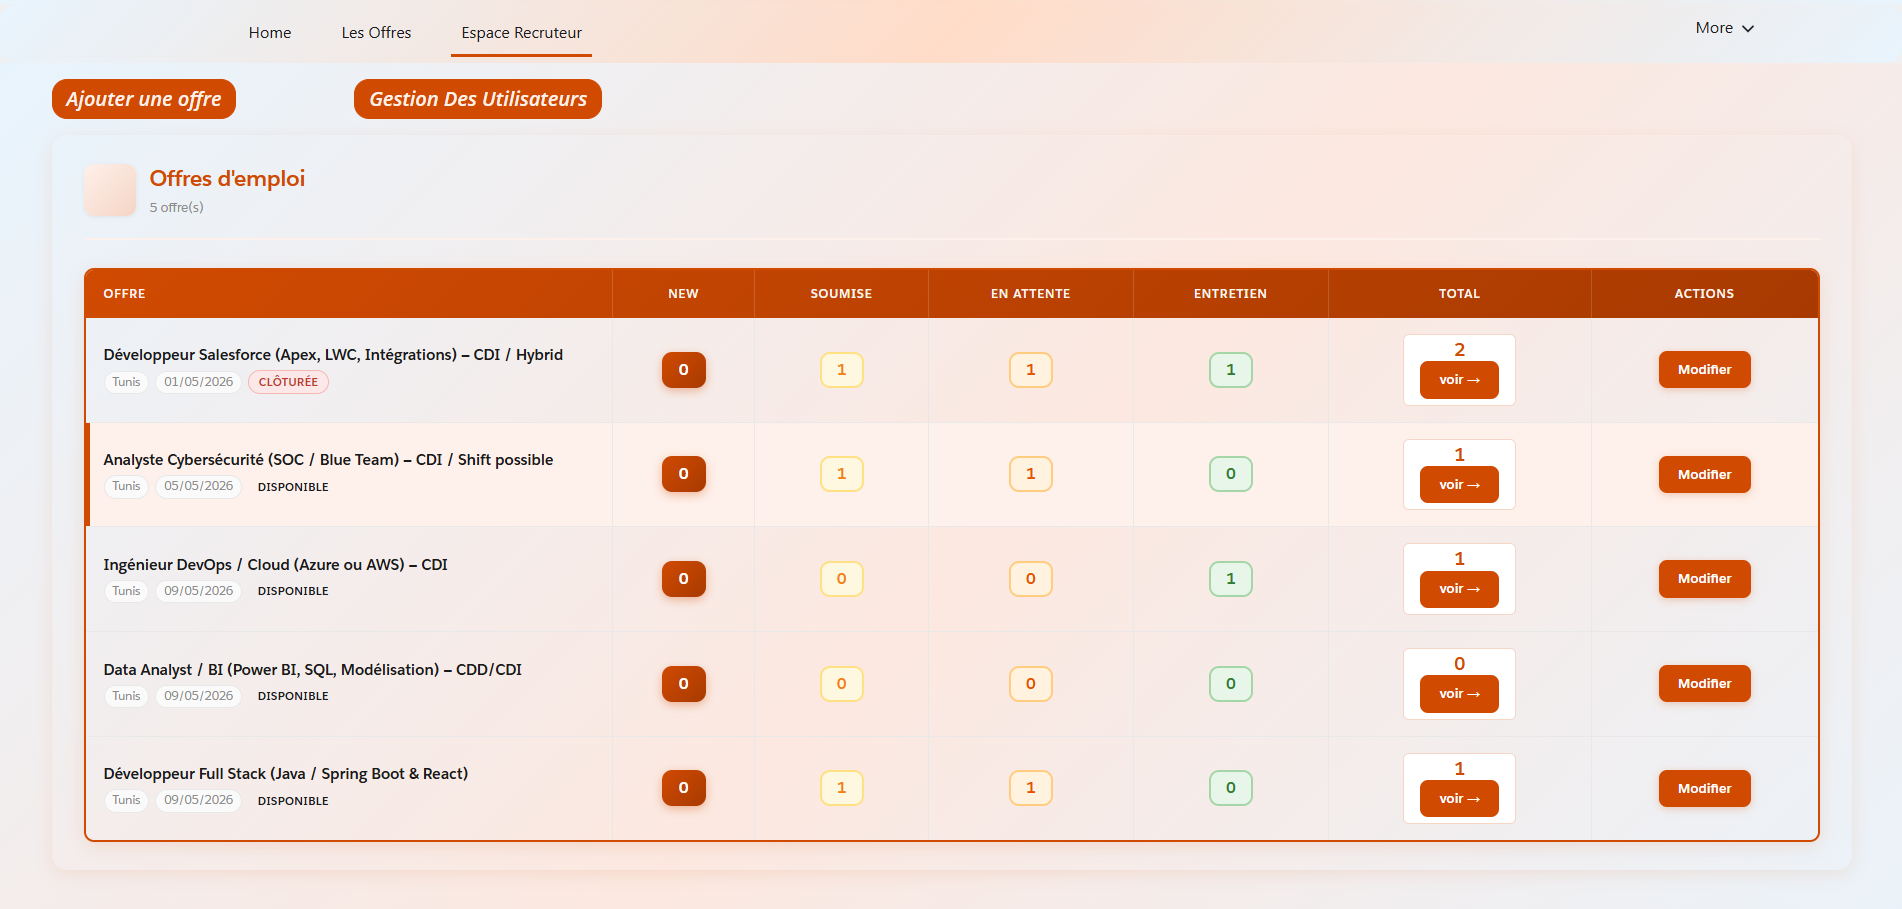
\includegraphics[width=\textwidth]{Figures/admindashbo.png}
             \caption{Tableau de bord de gestion (Lightning Experience)}
         \end{figure}
        \end{itemize}
    \begin{itemize}
        \item \textbf{Console d'Administration Salesforce (Setup) :} L'administrateur ne dispose pas d'une interface sur mesure ; il exploite la puissance du \textit{Setup} standard de Salesforce pour gérer les utilisateurs. C'est ici qu'il crée les comptes recruteurs en leur affectant le profil \textbf{Recruteur Platformdonc}.
         \begin{figure}[H]
             \centering
             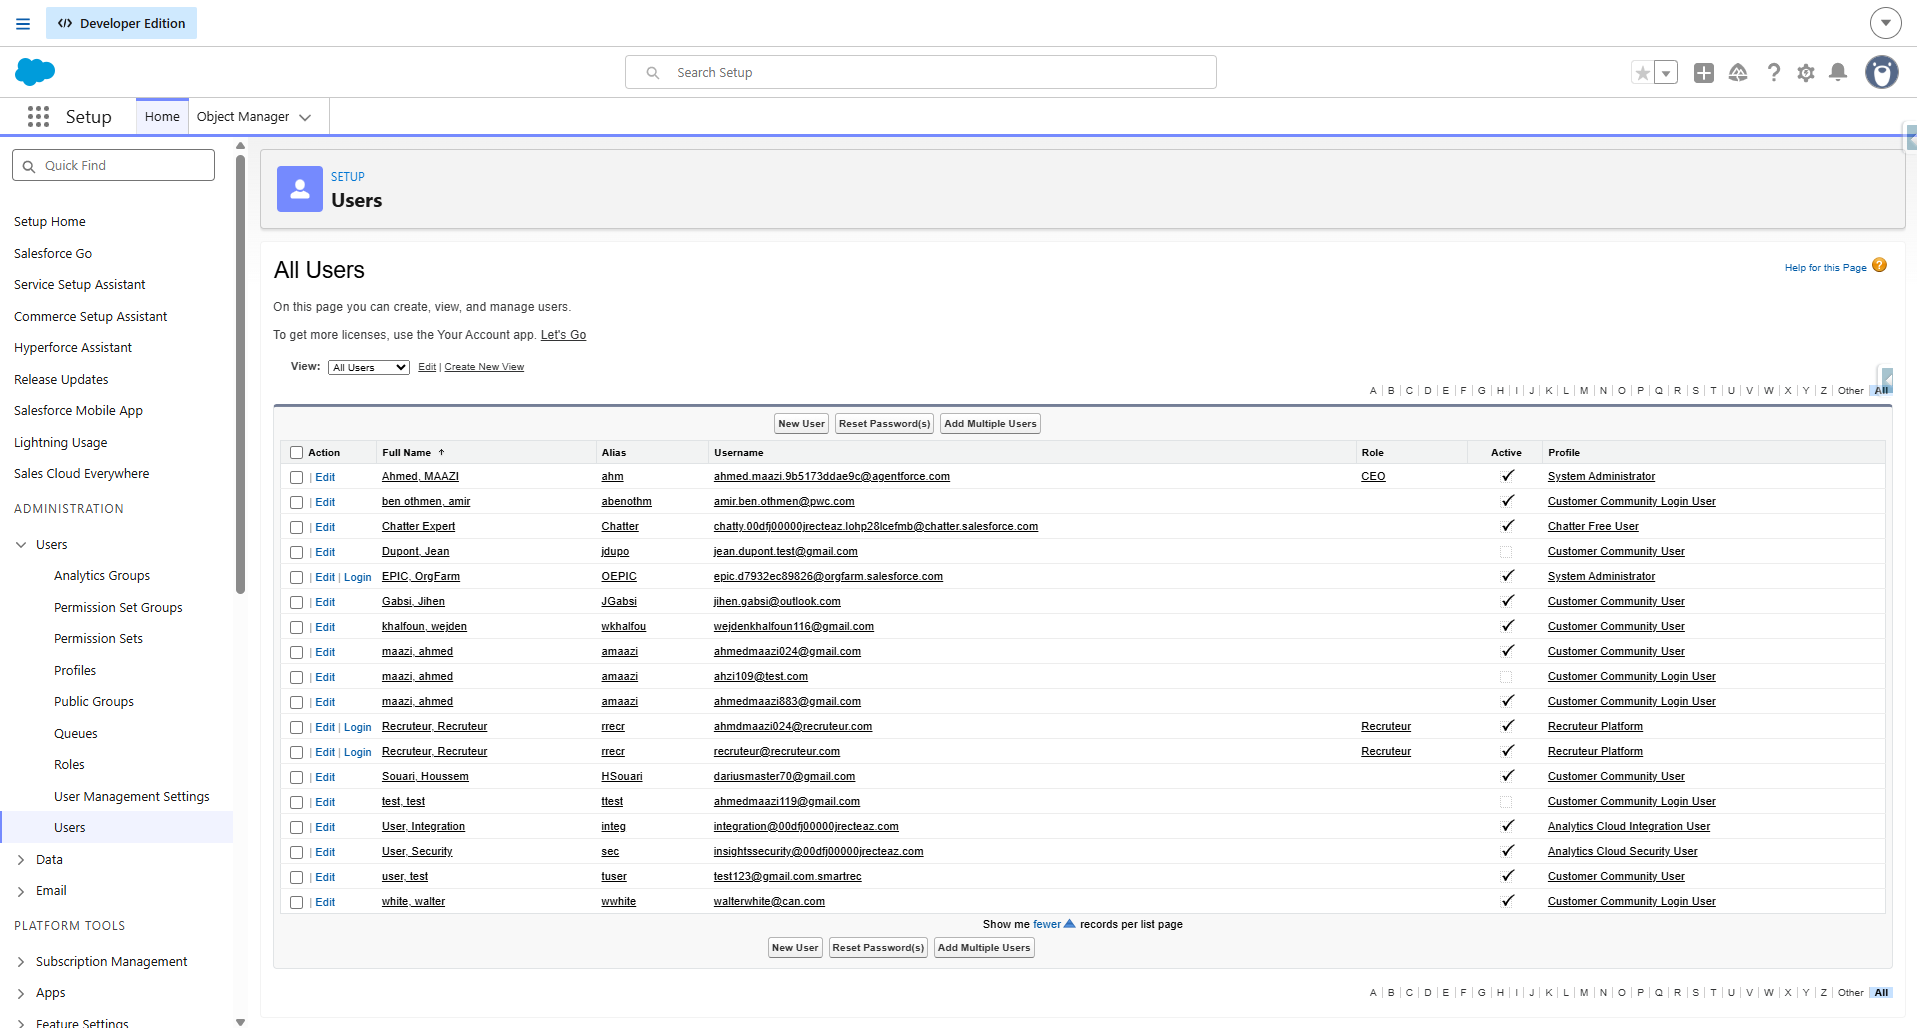
\includegraphics[width=\textwidth]{Figures/adminadduser1.png}
             \caption{Console de configuration standard pour la gestion des utilisateurs}
         \end{figure}
      \end{itemize}
\end{itemize}

\begin{itemize}
      \item\textbf{Suivi des candidatures par offre (Console Recruteur) :} 
Cette interface, au cœur de l'activité du recruteur, permet de consulter les détails d'une offre spécifique et de lister instantanément les candidats associés, facilitant ainsi le pilotage du workflow de recrutement.
          \begin{figure}[H]
              \centering
              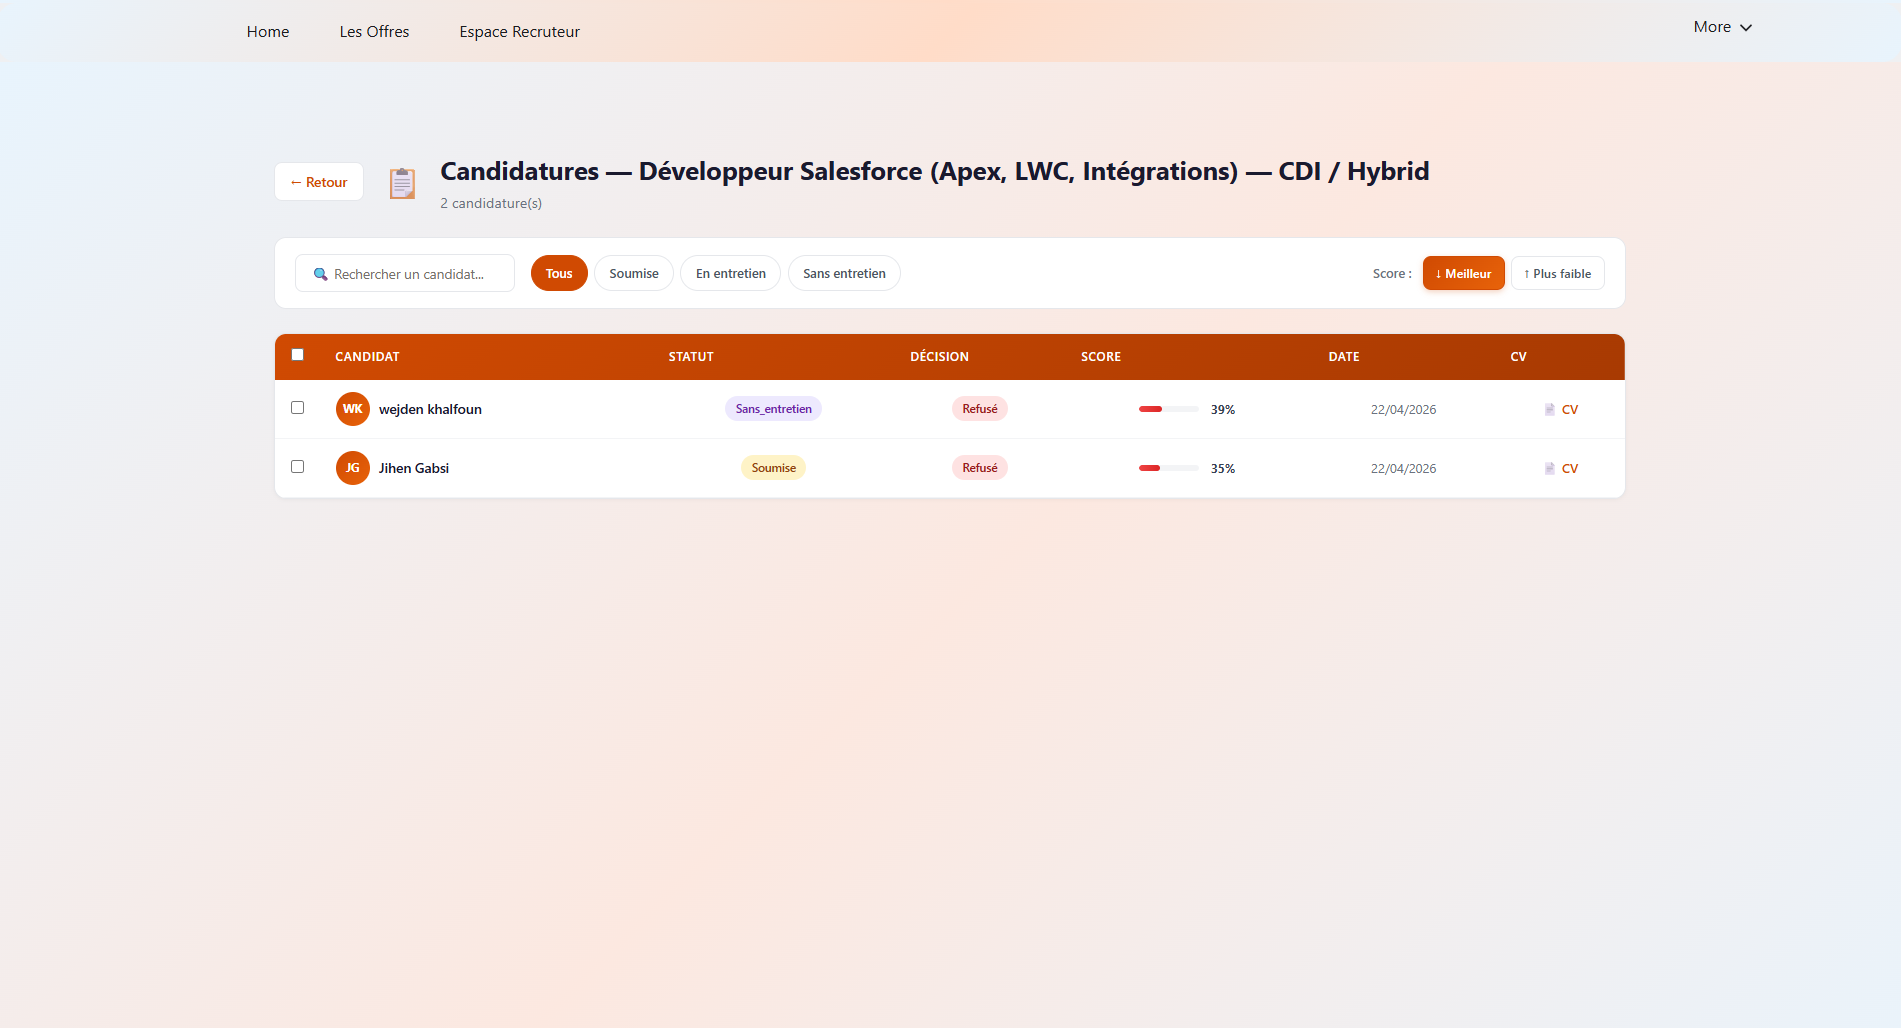
\includegraphics[width=\textwidth]{Figures/admintache.png}
              \caption{Interface de gestion des candidatures liées à une offre}
          \end{figure}
      \end{itemize}
\begin{itemize}
     \item\textbf{Interface d'inscription du candidat (Experience Cloud) :} 
Interface développée pour permettre aux nouveaux candidats de s'enregistrer de manière autonome. Elle valide les informations saisies et crée automatiquement un enregistrement de type Contact lié au compte utilisateur.
         \begin{figure}[H]
             \centering
             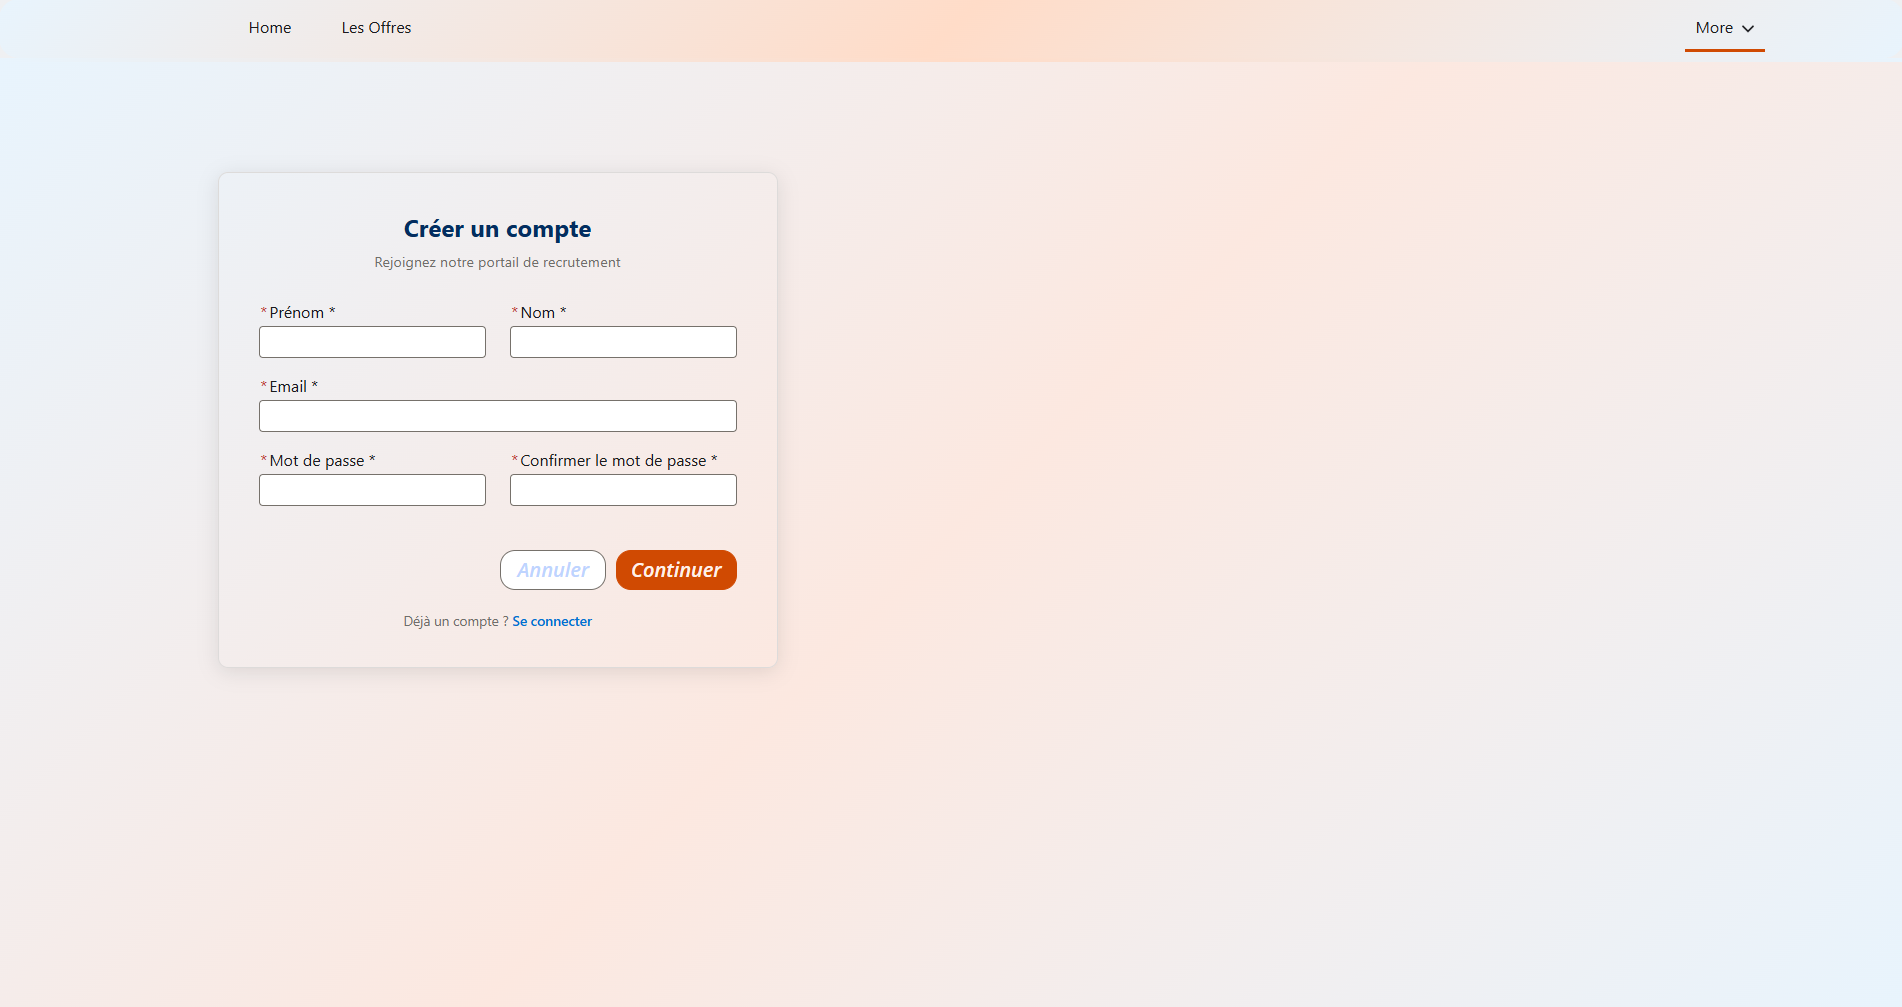
\includegraphics[width=\textwidth]{Figures/candidatinscri.png}
             \caption{Portail Candidat - Interface d'inscription}
         \end{figure}
     \end{itemize}
\begin{itemize}
      \begin{itemize}
          \item \textbf{Espace Candidat et Gestion du Profil :} Le portail offre une vue d'ensemble personnalisée où le candidat peut suivre l'état de ses candidatures et mettre à jour ses informations de profil (compétences, expériences) via des composants LWC dédiés.
          \begin{figure}[H]
              \centering
              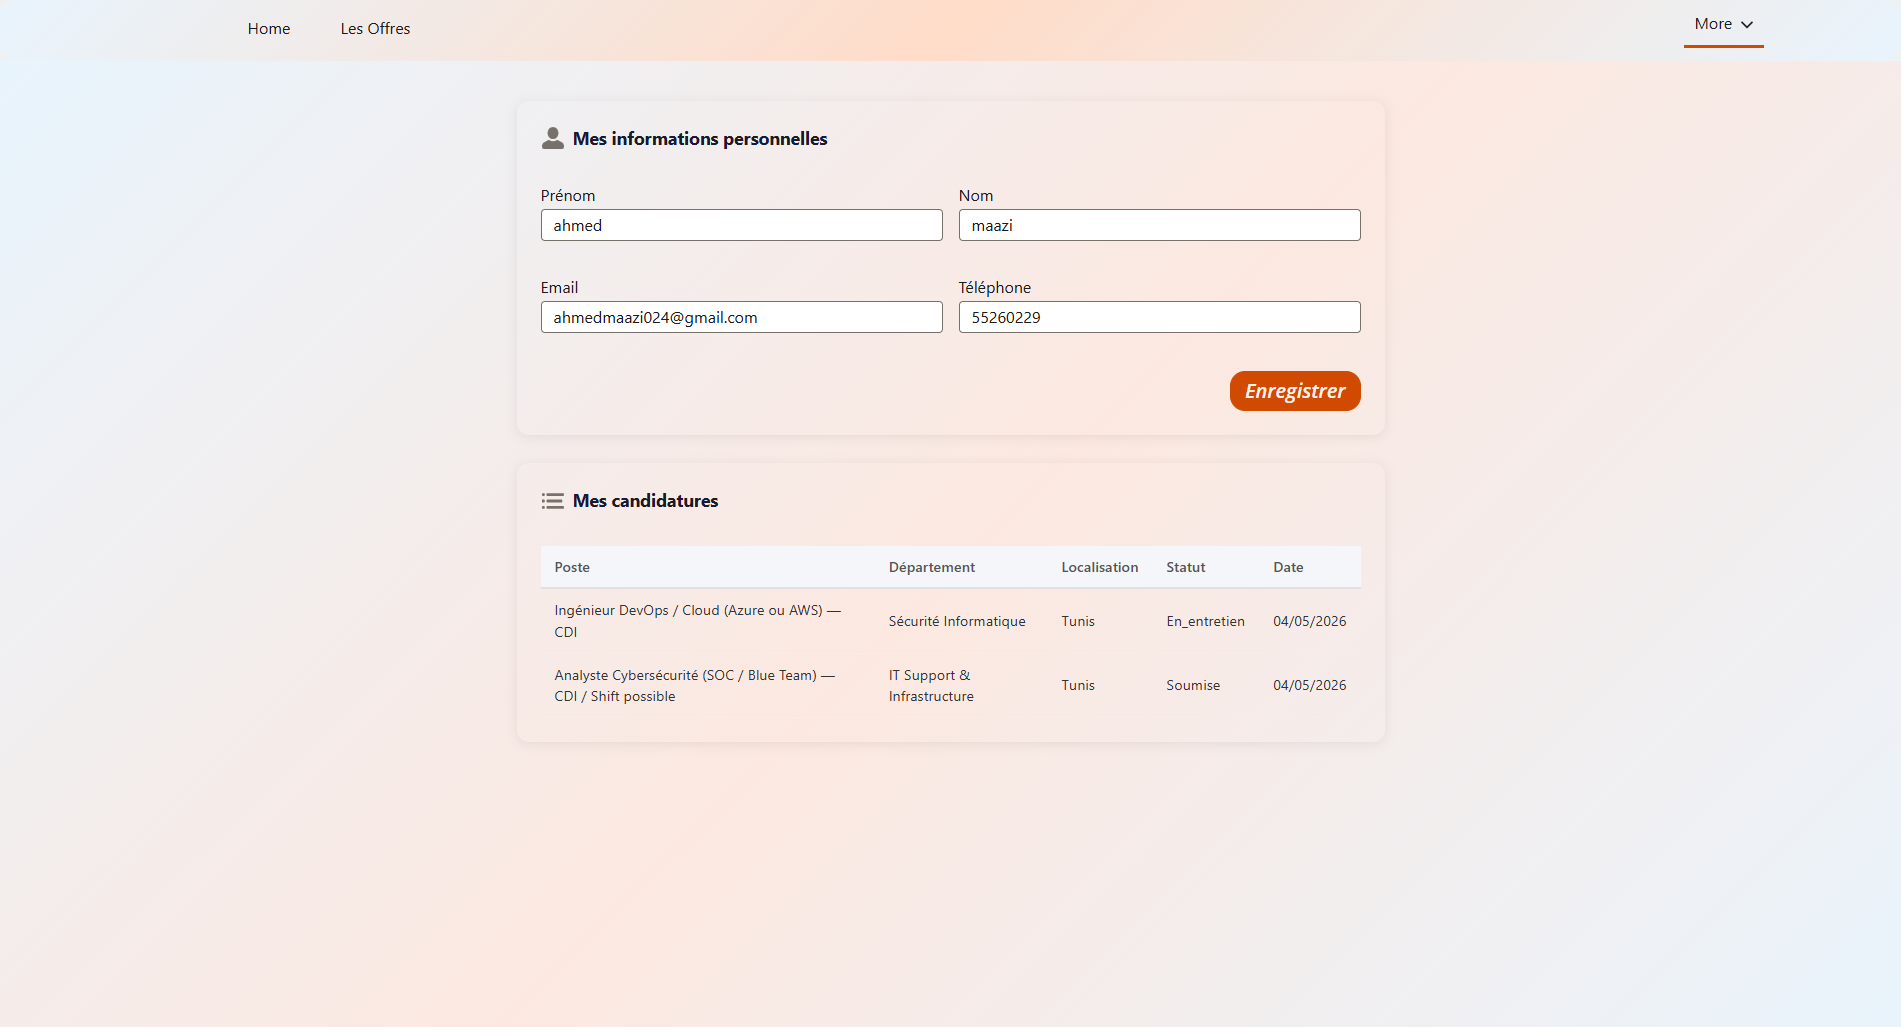
\includegraphics[width=\textwidth]{Figures/candidatprofil.png}
              \caption{Interface de gestion du profil candidat (LWC)}
          \end{figure}
      \end{itemize}
\end{itemize}



\section*{Conclusion}
\addcontentsline{toc}{section}{\protect\numberline{}Conclusion}
En définitive, ce premier sprint a permis de transformer une vision théorique de la sécurité en une infrastructure fonctionnelle sur Salesforce. En orchestrant les profils et les droits d'accès, nous avons créé un environnement de confiance, prêt à supporter les processus métiers complexes. Ce socle technique étant désormais stabilisé, le chapitre suivant se penchera sur le moteur même de SmartRec : la gestion automatisée du cycle de recrutement et l'analyse sémantique des profils.

 
\chead{CHAPITRE 4. SPRINT 2: Gestion de Recrutement et Candidatures}

\chapter{Sprint 2: Gestion de Recrutement et Candidatures}
\renewcommand{\mtctitle}{Sommaire}
\minitoc
	\newpage
\section*{Introduction}
Ce chapitre explore les étapes de la Sprint Gestion de Recrutement et Candidatures, avec un accent particulier sur la gestion des offres d’emploi et le processus de candidature. Nous débuterons par un aperçu du backlog, avant de détailler la conception, la mise en œuvre et d’illustrer le travail effectué à l’aide de captures d’écran.
\addcontentsline{toc}{section}{\protect\numberline{}Introduction}%
\section{Objectifs du Sprint}
L’objectif de cette sprint est de permettre la gestion des offres d’emploi par le responsable RH, ainsi que de faciliter la consultation et la soumission de candidatures par les candidats.

\section{Spécification des besoins}
\par Dans cette section, nous allons débuter par présenter le diagramme de cas d’utilisation de la sprint, suivi de l’exposition du backlog associé.
\subsection{Diagramme cas d’utilisation du Sprint 2}


\begin{figure}[H]
\centering
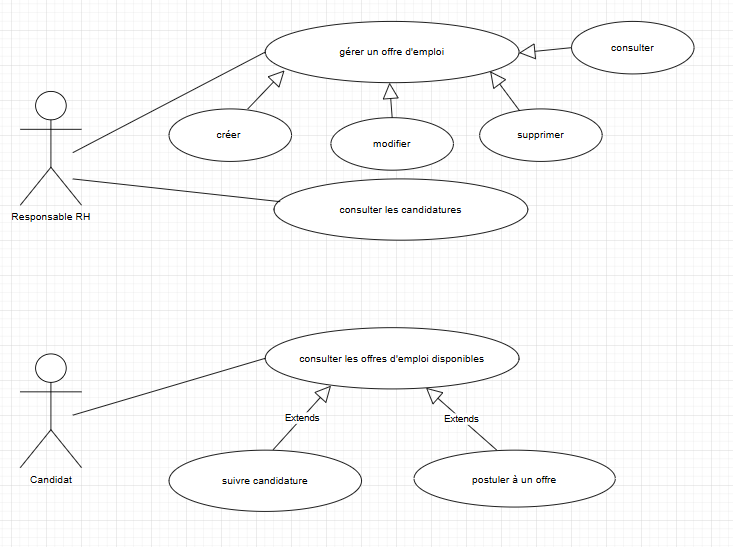
\includegraphics[width=14cm, height=11cm]{Figures/use case 2.png}
\caption{Diagramme cas d’utilisation du sprint 2}
\label{schema1}
\end{figure}
 
\subsection{ Sprint backlog du sprint 2}
Le tableau ci-dessous présente le sprint backlog établi pour le deuxième sprint. Il récapitule les différentes user stories sélectionnées, accompagnées de leurs identifiants uniques, ainsi que les tâches techniques à réaliser pour chacune. Ce tableau permet d’avoir une vision claire et structurée du travail prévu, en facilitant la planification, la répartition des responsabilités et le suivi de l’avancement tout au long du sprint.
\begin{table}[H]
\caption{Backlog du sprint 2}
\centering
\begin{tabular}{|p{1cm}|p{8cm}|p{8cm}|}
\hline
\textbf{ID} & \textbf{User Story} & \textbf{Tâches techniques} \\
\hline
US-8 & En tant que responsable RH, je veux créer, modifier et consulter des offres d’emploi afin d’attirer des candidats. 
& 
\begin{itemize}[leftmargin=*]
  \item Créer le modèle "Offre d'emploi".
  \item Développer le formulaire de création/modification.
  \item Implémenter les vues CRUD.
  \item Connecter à la base de données.
\end{itemize} \\
\hline
US-9 & En tant que candidat, je veux consulter toutes les offres d’emploi disponibles. 
& 
\begin{itemize}[leftmargin=*]
  \item Créer une page d'affichage des offres.
  \item Développer une API pour lister les offres.
  \item Mettre en place un filtre de recherche.
\end{itemize} \\
\hline
US-10 & En tant que candidat, je veux postuler à une offre d’emploi. 
& 
\begin{itemize}[leftmargin=*]
  \item Créer le modèle de "Candidature".
  \item Implémenter le bouton de candidature.
  \item Enregistrer la candidature dans la base.
\end{itemize} \\
\hline
US-11 & En tant que candidat, je veux suivre l’état de mes candidatures. 
& 
\begin{itemize}[leftmargin=*]
  \item Créer une vue "Mes candidatures".
  \item Ajouter un champ "état" (en cours, accepté, refusé).
\end{itemize} \\
\hline
US-12 & En tant que responsable RH, je veux accéder à la liste des candidatures. 
& 
\begin{itemize}[leftmargin=*]
  \item Créer la vue "Liste des candidatures".
  \item Créer un filtre de recherche.
  \item Lier avec le backend des candidatures.
\end{itemize} \\
\hline
\end{tabular}
\label{tab:sprint2_backlog}
\end{table}

\section{Analyse des besoins}
Avant de modéliser les fonctionnalités du système, il est essentiel de comprendre les besoins fonctionnels exprimés à travers les différents cas d’usage. La section suivante propose une description textuelle de ces cas d’utilisation, permettant de mieux cerner les interactions entre les utilisateurs et le système, et de poser les bases d’une modélisation cohérente.
    
\subsection{Description textuelle de cas d'utilisation}
    \begin{itemize}
        \item \textbf{Cas d'utilisation "Gérer une offre d'emploi": } La table 4.2 ci-dessous présente la description textuelle du cas d'utilisation « Gérer une offre d'emploi ».
    \end{itemize}
    \begin{table}[H]
    \caption{ Description textuelle du cas d’utilisation "Gérer une offre d'emploi"}
    \centering
    \begin{tabular}{|c|p{12cm}|}
    \hline
    \textbf{Titre} & Gérer une offre d'emploi \\
    \hline
    \textbf{Objectif} & Permettre au responsable RH de gérer les offres d’emploi (création, modification, archivage). \\
    \hline
    \textbf{Acteur}& Responsable RH\\
    \hline
    \textbf{Pré-condition} & Le responsable RH doit être authentifié et avoir les droits d’accès nécessaires.
    \\
    \hline
    \textbf{Post-condition} & Les modifications ou archivages des offres sont enregistrés dans le système.\\
    \hline
    \textbf{Scénario nominal} & 1. Le responsable RH accède à l’interface de gestion des offres. \newline
    2. Il sélectionne une action (créer, modifier, archiver).\newline
    3. Il entre ou modifie les détails de l’offre (titre, description, etc.).
    \newline
    4. Le système valide et enregistre les changements.\\
    \hline
    \end{tabular}
    \label{tab:user_stories}
\end{table}

\begin{itemize}
        \item \textbf{Cas d'utilisation "Consulter les candidatures": } La table 4.3 ci-dessous présente la description textuelle du cas d'utilisation « Consulter les candidatures ».
    \end{itemize}
    \begin{table}[H]
    \caption{ Description textuelle du cas d’utilisation "consulter les candidatures"}
    \centering
    \begin{tabular}{|c|p{12cm}|}
    \hline
    \textbf{Titre} & Consulter les candidatures \\
    \hline
    \textbf{Objectif} & Permettre au responsable RH de visualiser la liste des candidatures reçues pour une offre. \\
    \hline
    \textbf{Acteur}& Responsable RH\\
    \hline
    \textbf{Pré-condition} & Une offre d’emploi doit exister et des candidatures doivent avoir été soumises.
    \\
    \hline
    \textbf{Post-condition} & La liste des candidatures est affichée avec les détails des candidats.\\
    \hline
    \textbf{Scénario nominal} & 1. Le responsable RH accède à la gestion des offres. \newline
    2. Il sélectionne une offre spécifique.\newline
    3. Le système affiche la liste des candidatures.
    \newline
    4. Il consulte les détails des candidatures.\\
    \hline
    \end{tabular}
    \label{tab:user_stories}
\end{table}

\begin{itemize}
        \item \textbf{Cas d'utilisation "Consulter les offres d'emploi": } La table 4.4 ci-dessous présente la description textuelle du cas d'utilisation « Consulter les offres d'emploi ».
    \end{itemize}
    \begin{table}[H]
    \caption{ Description textuelle du cas d’utilisation "Consulter les offres d'emploi"}
    \centering
    \begin{tabular}{|c|p{12cm}|}
    \hline
    \textbf{Titre} & Consulter les offres d'emploi \\
    \hline
    \textbf{Objectif} & Permettre au candidat de visualiser les offres d’emploi disponibles sur la plateforme. \\
    \hline
    \textbf{Acteur}& Candidat\\
    \hline
    \textbf{Pré-condition} & Le candidat doit avoir accès à la plateforme .
    \\
    \hline
    \textbf{Post-condition} & La liste des offres d’emploi est affichée au candidat.\\
    \hline
    \textbf{Scénario nominal} & 1. Le candidat accède à la section des offres. \newline
    2. Il navigue dans la liste des offres.\newline
    3. Le système affiche les détails de chaque offre.
    \newline
    4. Il consulte les informations.\\
    \hline
    \end{tabular}
    \label{tab:user_stories}
\end{table}

\begin{itemize}
        \item \textbf{Cas d'utilisation "Postuler à une offre": } La table 4.5 ci-dessous présente la description textuelle du cas d'utilisation « Postuler à une offre ».
    \end{itemize}
    \begin{table}[H]
    \caption{ Description textuelle du cas d’utilisation "Postuler à une offre"}
    \centering
    \begin{tabular}{|c|p{12cm}|}
    \hline
    \textbf{Titre} & Postuler à une offre \\
    \hline
    \textbf{Objectif} & Permettre au candidat de soumettre une candidature pour une offre d’emploi. \\
    \hline
    \textbf{Acteur}& Candidat\\
    \hline
    \textbf{Pré-condition} & Le candidat doit avoir un compte actif et une offre doit être disponible.
    \\
    \hline
    \textbf{Post-condition} & La candidature est envoyée et enregistrée dans le système avec le profil du candidat.\\
    \hline
    \textbf{Scénario nominal} & 1. Le candidat accède à une offre d’emploi.\newline
    2. Il clique sur l’option "Postuler".\newline
    3. Le système soumet automatiquement son profil comme candidature.
    \newline
    4. Le système confirme l’envoi de la candidature.\\
    \hline
    \end{tabular}
    \label{tab:user_stories}
\end{table}

\begin{itemize}
        \item \textbf{Cas d'utilisation "Suivre les candidatures": } La table 4.6 ci-dessous présente la description textuelle du cas d'utilisation « Suivre les candidatures ».
    \end{itemize}
    \begin{table}[H]
    \caption{ Description textuelle du cas d’utilisation "Suivre les candidatures"}
    \centering
    \begin{tabular}{|c|p{12cm}|}
    \hline
    \textbf{Titre} & Suivre les candidatures \\
    \hline
    \textbf{Objectif} & Permettre au candidat de suivre l’état de ses candidatures soumises. \\
    \hline
    \textbf{Acteur}& Candidat\\
    \hline
    \textbf{Pré-condition} & Le candidat doit avoir un compte actif, un profil complété et au moins une candidature soumise.
    \\
    \hline
    \textbf{Post-condition} & L’état des candidatures du candidat est affiché et mis à jour dans le système.\\
    \hline
    \textbf{Scénario nominal} & 1. Le candidat se connecte à l’application.\newline
    2. Il accède à la section de ses candidatures.\newline
    3. Le système affiche la liste de ses candidatures avec leur état (en attente, accepté, refusé).
    \newline
    4. Il consulte les détails de chaque candidature.\\
    \hline
    \end{tabular}
    \label{tab:user_stories}
\end{table}

\section{Conception}
\hspace{0.5cm}\textbf Dans cette section, nous discutons de la conception du deuxième sprint. nous Commençons par le diagramme de classes du sprint. Ensuite, nous examinons la modélisation de quelques diagrammes de séquences. 



   
\subsection{Diagrammes de séquences}
Dans le cadre de l’analyse dynamique du système, un diagramme de séquence a été réalisé pour chaque fonctionnalité clé développée lors des sprints. Le diagramme ci-dessous illustre spécifiquement le scénario du cas d'utilisation « Gérer un offre d'emploi », permettant de visualiser les interactions entre le responsable rh et le système lors de la création d’un nouvel offre d'emploi.
\subsubsection{ Diagramme de séquence au scénario : «Gérer un offre d'emploi»}
Cette figure illustre le déroulement du scénario associé à ce cas d'utilisation.
     \begin{figure}[H]
    \centering
   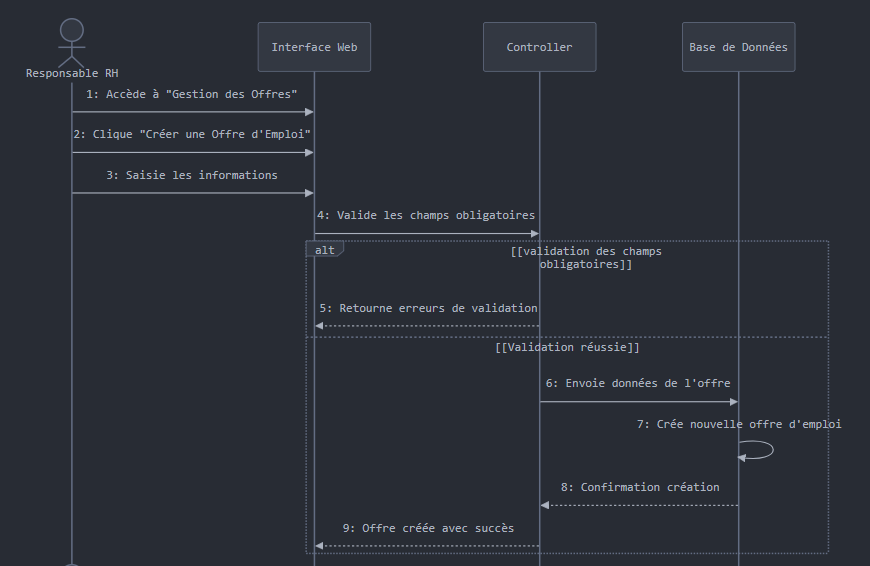
\includegraphics[width=18cm, height=18cm]{Figures/seq2.png}
    \caption{Diagramme de séquence détaillé au scénario «Gérer un offre d'emploi»}

\end{figure}
\section{Réalisation: interfaces utilisateur dans RhNova }
Dans cette partie, nous illustrons les principales interfaces conçues dans le cadre du processus de recrutement. Elles permettent aux responsables RH de gérer les offres et de suivre les candidatures, tandis que les candidats peuvent consulter les annonces disponibles et suivre l’état de leurs demandes.
\vspace{5mm}
\begin{itemize}
     \begin{itemize}
      \item \textbf{ Gestion des offres d'emploi : }Cette interface permet au responsable RH de créer, consulter et gérer les offres d’emploi. Il peut y renseigner les détails du poste (titre, département, type de contrat, lieu, salaire, date limite, etc.) ainsi que la description et les exigences du poste. Les offres actives est également visible et modifiable depuis cet espace.
         \begin{figure}[H]
             \centering
             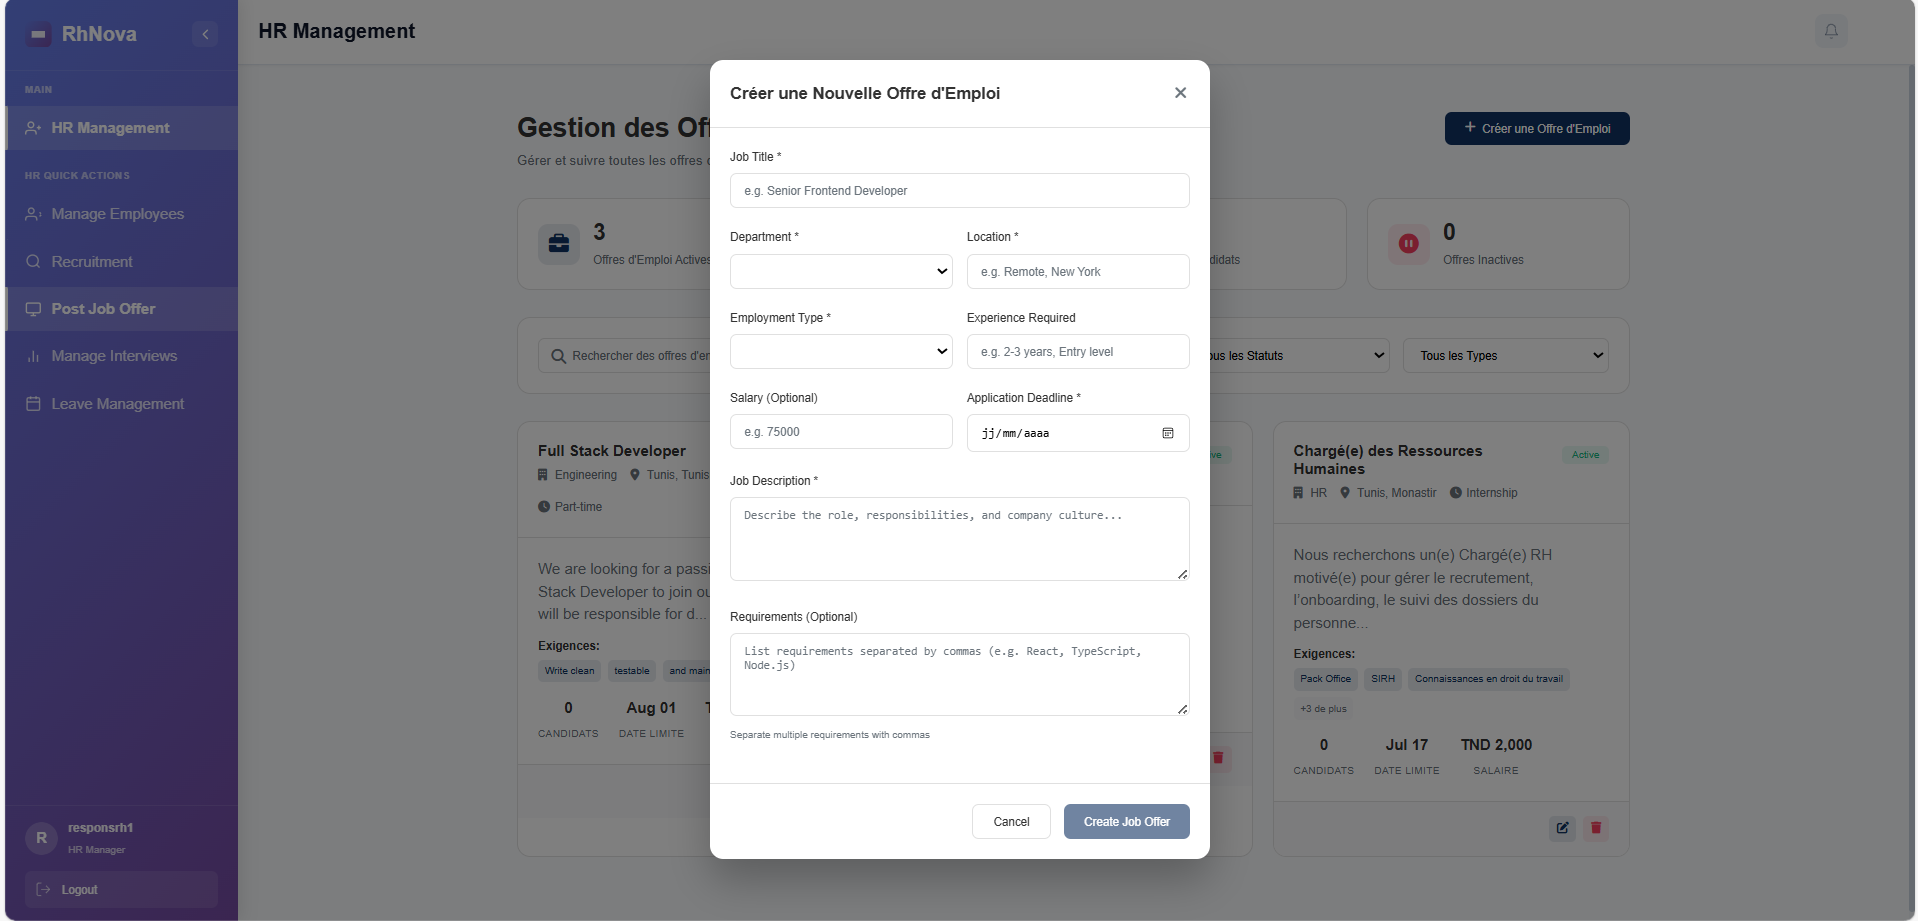
\includegraphics[width=\textwidth]{Figures/responsjoboffer.png}
             \caption{Page de gestion d'offre d'emploi}
         \end{figure}
     \end{itemize}
\end{itemize}
\begin{itemize}
     \item\textbf{Consultation des candidatures : }
Cette interface permet au responsable RH d'accéder aux candidatures reçues après filtrage automatique des CV par le système ATS. Il peut consulter les profils détaillés des candidats pour chaque offre, ce qui facilite l’évaluation et la présélection.
         \begin{figure}[H]
             \centering
             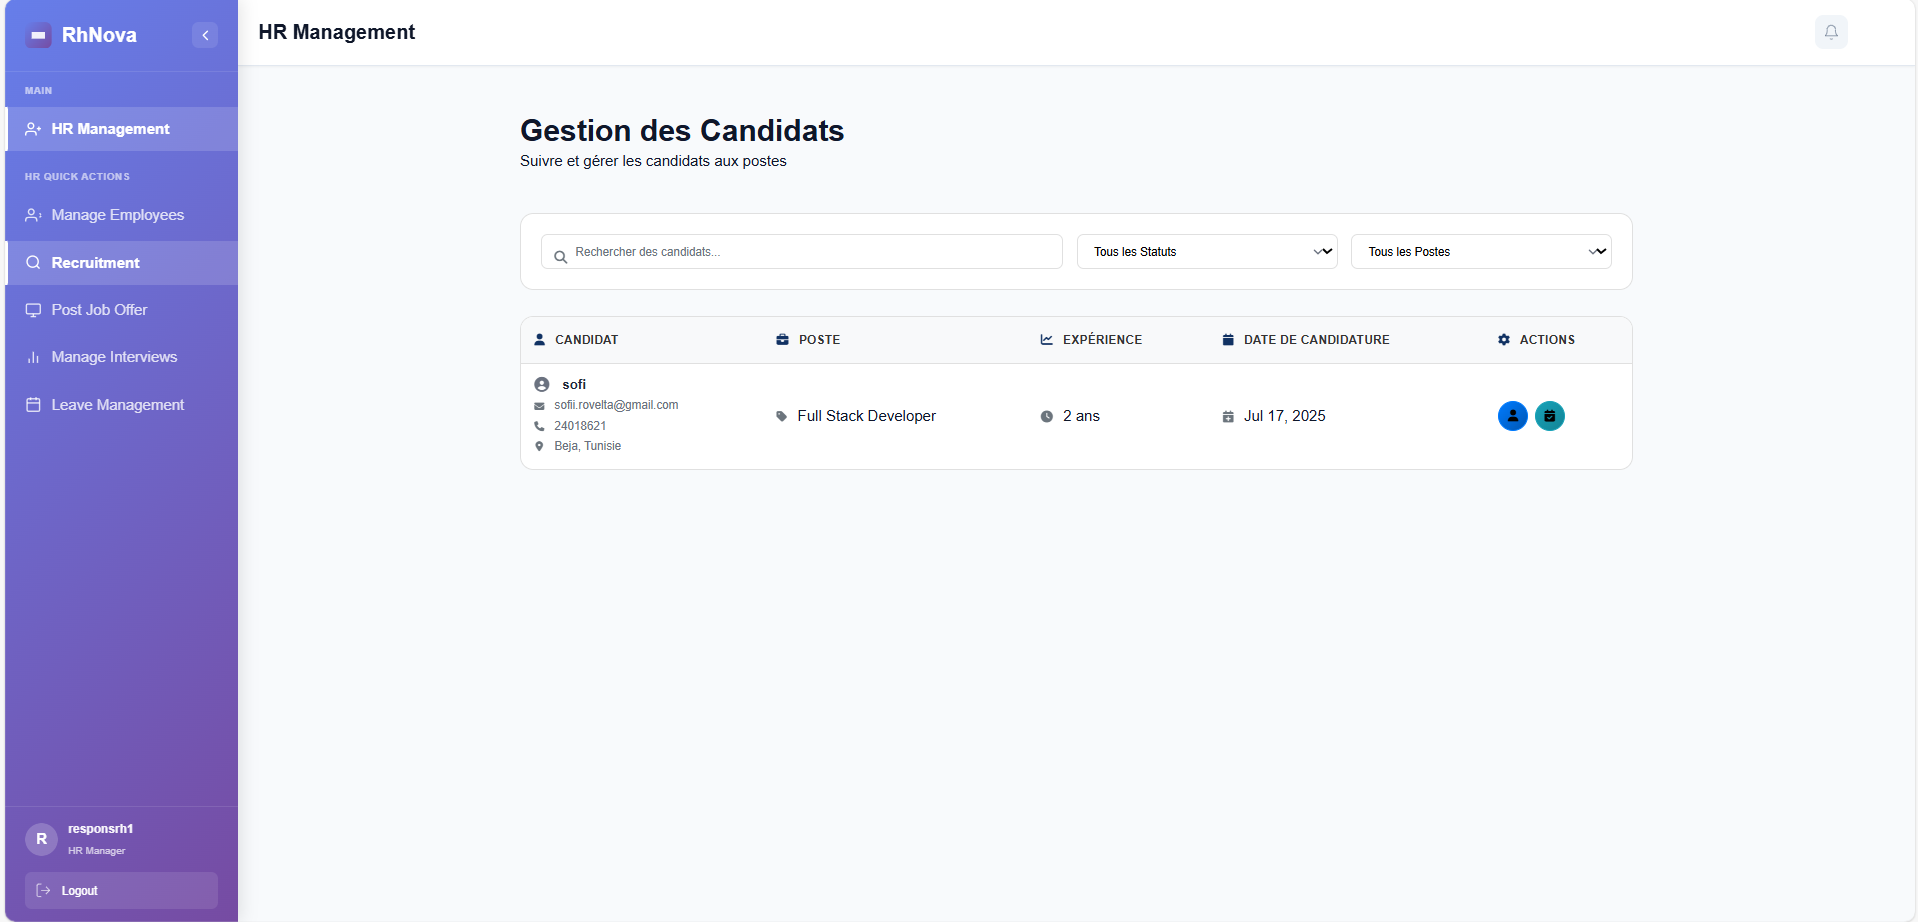
\includegraphics[width=\textwidth]{Figures/responscandidature.png}
             \caption{Liste des candidatures}
         \end{figure}
\end{itemize}
\begin{itemize}
     \item\textbf{Consultation des offres : }
Cette interface permet au candidat de consulter la liste des offres d’emploi disponibles avec leurs détails (poste, lieu, compétences, type de contrat). Il peut voir les informations complètes d’une offre et postuler directement en ligne.
         \begin{figure}[H]
             \centering
             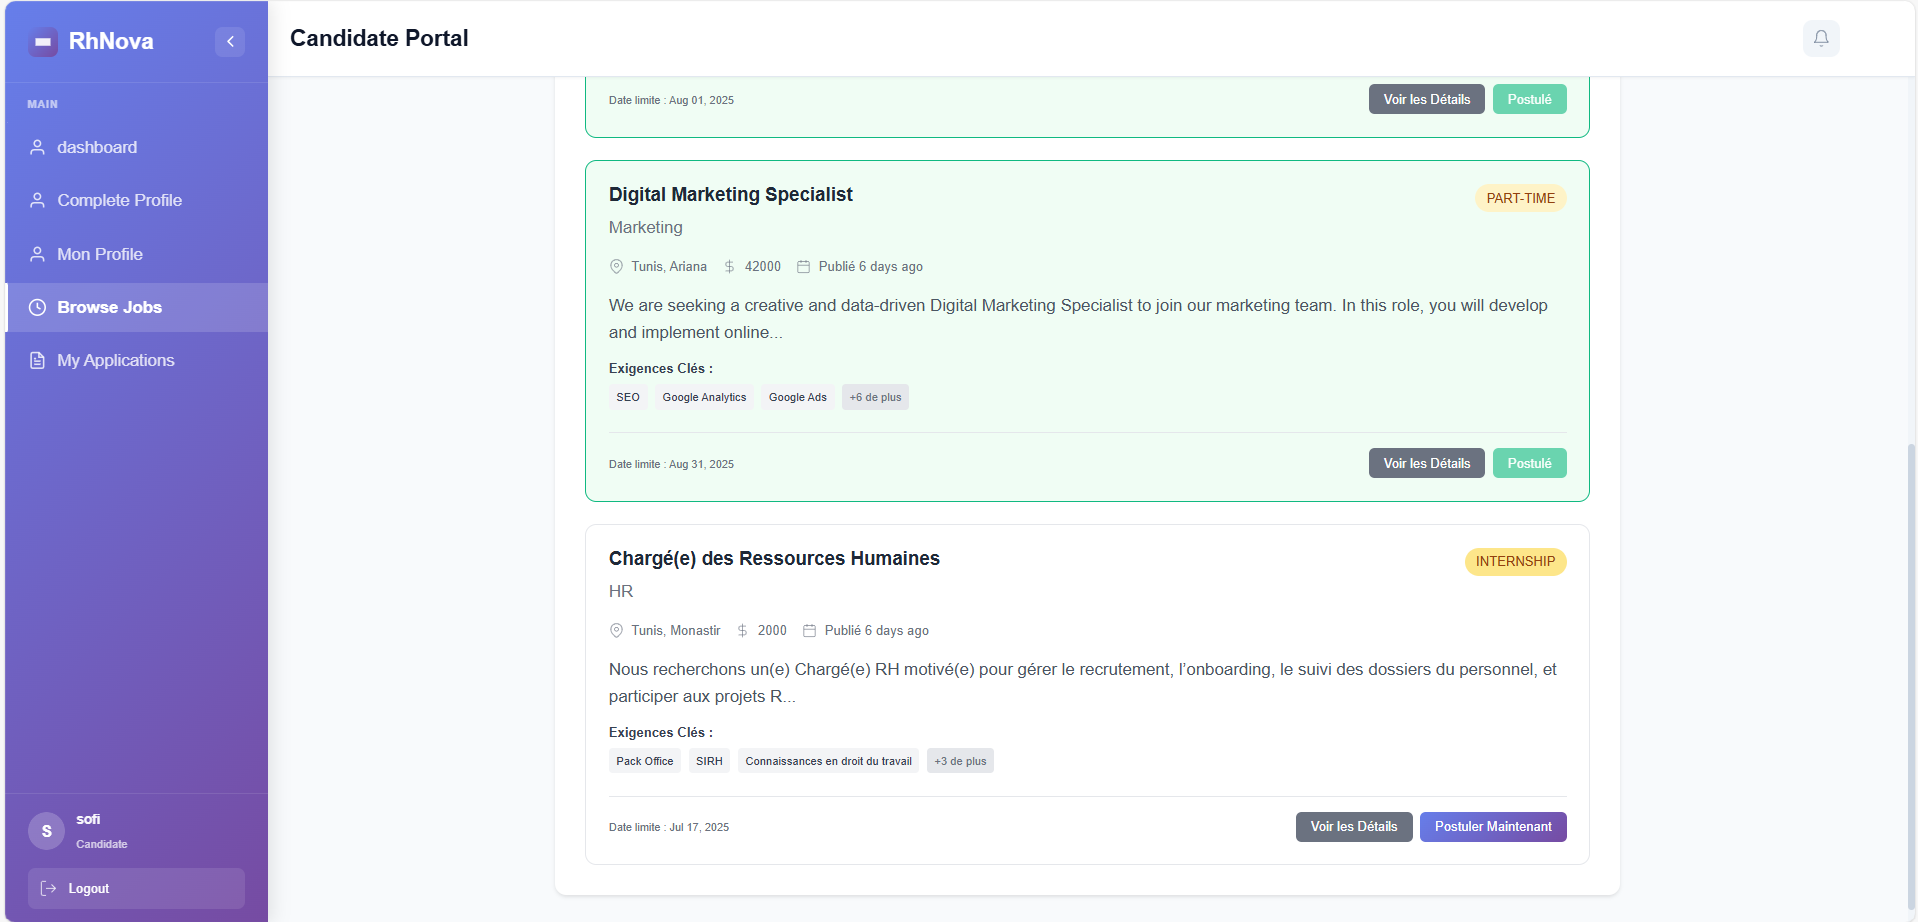
\includegraphics[width=\textwidth]{Figures/candidatoffre.png}
             \caption{Liste des offres}
         \end{figure}
\end{itemize}
\begin{itemize}
     \item\textbf{Suivi des candidatures : }
Cette interface permet au candidat de suivre l’avancement de ses candidatures. Il peut consulter le statut de chaque étape du processus (soumission, entretien, décision finale) et accéder aux détails de ses entretiens, y compris la date, l’heure et le type d’entretien, ainsi qu’un lien vers l’enregistrement si disponible.
         \begin{figure}[H]
             \centering
             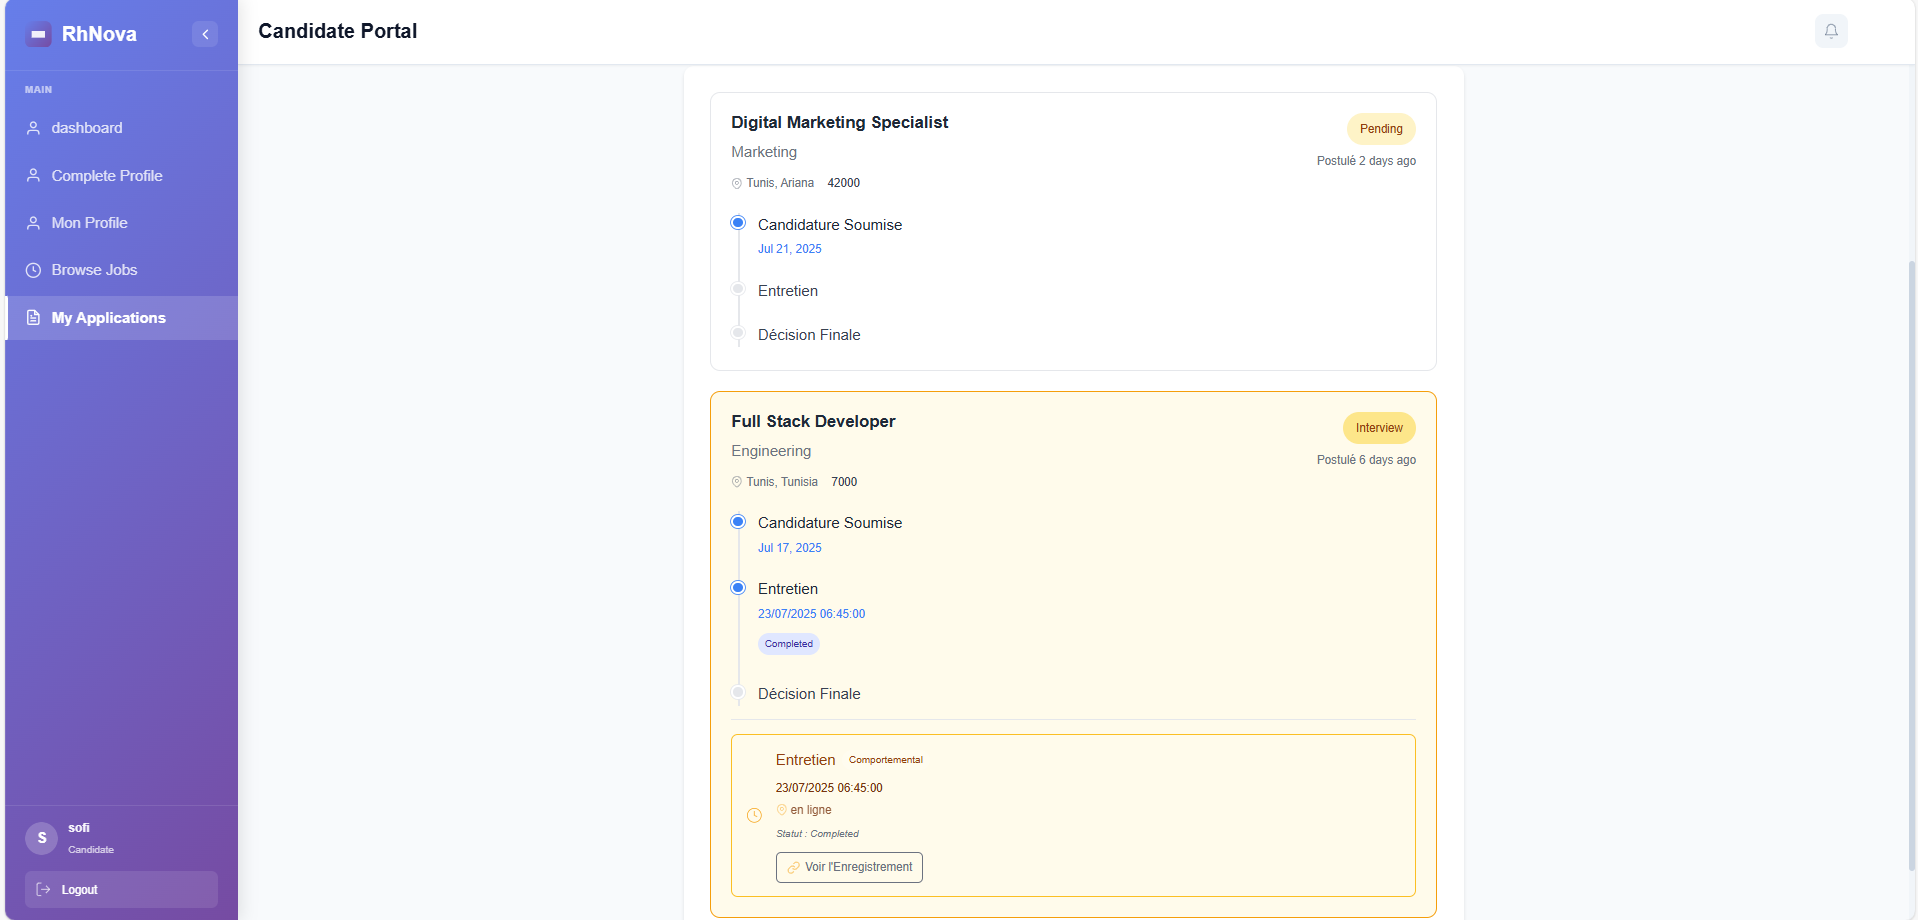
\includegraphics[width=\textwidth]{Figures/candidatsuivre.png}
             \caption{Suivi des candidatures}
         \end{figure}
     \end{itemize}

\section*{Conclusion}
En conclusion, ce chapitre a encadré la Sprint Gestion de Recrutement et Candidatures, en établissant les objectifs et détaillant le backlog, tout en exposant les diagrammes de cas d’utilisation, classes et de séquences. Les descriptions textuelles et captures d’écran ont confirmé la mise en œuvre réussie, posant des fondations robustes pour les phases de recrutement futures.Dans le chapitre suivant, nous aborderons les détails du troisième sprint " Gestion des Entretiens et ATS".
\addcontentsline{toc}{section}{\protect\numberline{}Conclusion}%




 
\chead{CHAPITRE 5 . SPRINT 3:  \textbf{Gestion des Entretiens et ATS}}

\chapter{Sprint 3: Gestion des Entretiens et ATS}
\renewcommand{\mtctitle}{Sommaire}
\minitoc
\newpage
\section*{Introduction}
\addcontentsline{toc}{section}{\protect\numberline{}Introduction}%
Ce chapitre explore les étapes de la Sprint Gestion des Entretiens et ATS, avec un accent particulier sur la gestion des processus d’entretien et l’utilisation d’un système ATS. Nous débuterons par un aperçu du backlog, avant de détailler la conception, la mise en œuvre et d’illustrer le travail effectué à l’aide de captures d’écran.
\section{Objectifs du Sprint}
L’objectif de cette sprint est de mettre en place un système ATS pour filtrer les CV, gérer les statuts des candidats, planifier et modifier les entretiens, ainsi qu’envoyer des mails automatiques.


\section{Spécification des besoins}
\par Dans cette section, nous allons débuter par présenter le diagramme de cas d’utilisation de la sprint, suivi de l’exposition du backlog associé.
\subsection{Diagramme cas d’utilisation du Sprint 3}


\begin{figure}[H]
\centering
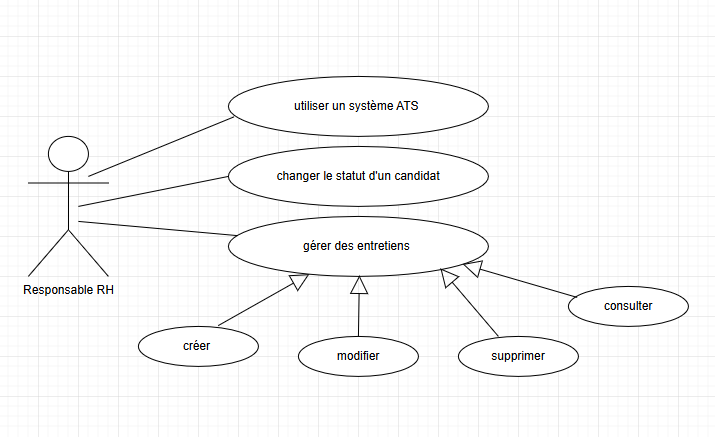
\includegraphics[width=18cm, height=9cm]{Figures/use case 3.png}
\caption{Diagramme cas d’utilisation du sprint 3}
\label{schema1}
\end{figure}


\subsection{ Sprint Backlog du sprint 3}
Le tableau suivant illustre le sprint backlog établi pour le troisième sprint. Il récapitule les différentes user stories sélectionnées, accompagnées de leurs identifiants uniques, ainsi que les tâches techniques à réaliser pour chacune. Ce tableau permet d’avoir une vision claire et structurée du travail prévu, en facilitant la planification, la répartition des responsabilités et le suivi de l’avancement tout au long du sprint.



\begin{table}[H]
\caption{Backlog du sprint 3}
\centering
\begin{tabular}{|p{1cm}|p{8cm}|p{8cm}|}
\hline
\textbf{ID} & \textbf{User Story} & \textbf{Tâches techniques} \\
\hline
US-13 & En tant que responsable RH, je veux utiliser un système ATS pour filtrer automatiquement les CV et prioriser les profils. 
& 
\begin{itemize}[leftmargin=*]
  \item Développer un algorithme de filtrage des CV.
  \item Implémenter un système de score/priorité.
  \item Créer l'interface de visualisation des résultats filtrés.
\end{itemize} \\
\hline
US-14 & En tant que responsable RH, je veux changer le statut d’un candidat. 
& 
\begin{itemize}[leftmargin=*]
  \item Ajouter un champ "statut" dans le modèle "Candidature".
  \item Connecter l’action à la base de données.
\end{itemize} \\
\hline
US-15 & En tant que responsable RH, je veux planifier des entretiens. 
& 
\begin{itemize}[leftmargin=*]
  \item Créer un formulaire de planification d’entretien.
\end{itemize} \\
\hline
US-16 & En tant que responsable RH, je veux modifier ou supprimer un entretien déjà planifié. 
& 
\begin{itemize}[leftmargin=*]
  \item Créer les options "modifier" et "supprimer" sur le calendrier.
  \item Gérer les mises à jour et suppressions côté base.
  \item Afficher les messages de confirmation.
\end{itemize} \\
\hline
\end{tabular}
\label{tab:sprint3_backlog}
\end{table}




\section{Analyse des besoins}
Avant de modéliser les fonctionnalités du système, il est essentiel de comprendre les besoins fonctionnels exprimés à travers les différents cas d’usage. La section suivante propose une description textuelle de ces cas d’utilisation, permettant de mieux cerner les interactions entre les utilisateurs et le système, et de poser les bases d’une modélisation cohérente. 
    
\subsection{Description textuelle de cas d'utilisation}

     \item \textbf{Cas d'utilisation "Utiliser un système ATS": } La table 5.2 ci-dessous présente la description textuelle du cas d'utilisation « Utiliser un système ATS ».

 \begin{table}[H]
 \caption{ Description textuelle du cas d’utilisation "Utiliser un système ATS"}
    \centering
    \begin{tabular}{|c|p{12cm}|}
    \hline
    \textbf{Titre} & Utiliser un système ATS \\
    \hline
    \textbf{Objectif} & Permettre au responsable RH d’utiliser un système ATS pour filtrer automatiquement les CV et prioriser les profils des candidats. \\
    \hline
    \textbf{Acteur}& Responsable RH\\
    \hline
    \textbf{Pré-condition} & Le responsable RH doit être authentifié et le système ATS doit être configuré.
    \\
    \hline
    \textbf{Post-condition} & Les CV sont filtrés et une liste de profils prioritaires est générée.\\
    \hline
    \textbf{Scénario nominal} & 1. Le responsable RH accède à l’interface de candidatures \newline
    2. Le système ATS filtre automatiquement les candidatures.\newline
    3. La liste des candidatures filtrées s’affiche directement.
    \newline
    4. Il consulte les résultats prioritaires.\\
    \hline
    \end{tabular}
    \label{tab:user_stories}
\end{table}


     \item \textbf{Cas d'utilisation "Changer le statut d'un candidat": } La table 5.3 ci-dessous présente la description textuelle du cas d'utilisation « Changer le statut d'un candidat ».

 \begin{table}[H]
 \caption{ Description textuelle du cas d’utilisation "Changer le statut d'un candidat"}
    \centering
    \begin{tabular}{|c|p{12cm}|}
    \hline
    \textbf{Titre} & Changer le statut d'un candidat \\
    \hline
    \textbf{Objectif} & Permettre au responsable RH de modifier le statut d’un candidat (en attente, entretien, accepté, refusé). \\
    \hline
    \textbf{Acteur}& Responsable RH\\
    \hline
    \textbf{Pré-condition} & Une candidature doit exister dans le système.
    \\
    \hline
    \textbf{Post-condition} & Le nouveau statut du candidat est mis à jour et visible.\\
    \hline
    \textbf{Scénario nominal} & 1. Le responsable RH accède à la gestion des entretiens. \newline
    2. Il planifie un entretien pour un candidat.\newline
    3. Le système change automatiquement le statut (ex. "En entretien").
    \newline
    4. Après l’entretien, il enregistre le résultat.
    5. Le système met à jour le statut automatiquement (ex. "Accepté" ou "Refusé").\\
    \hline
    \end{tabular}
    \label{tab:user_stories}
\end{table}

     \item \textbf{Cas d'utilisation "Gérer des entretiens": } La table 5.4 ci-dessous présente la description textuelle du cas d'utilisation « Gérer des entretiens ».

 \begin{table}[H]
 \caption{ Description textuelle du cas d’utilisation "Gérer des entretiens"}
    \centering
    \begin{tabular}{|c|p{12cm}|}
    \hline
    \textbf{Titre} & Gérer des entretiens \\
    \hline
    \textbf{Objectif} & Permettre au responsable RH de créer, modifier, supprimer et consulter les entretiens planifiés. \\
    \hline
    \textbf{Acteur}& Responsable RH\\
    \hline
    \textbf{Pré-condition} & Le responsable RH doit être authentifié et un candidat doit être sélectionné.
    \\
    \hline
    \textbf{Post-condition} & Les modifications ou suppressions des entretiens sont enregistrées dans le système.\\
    \hline
    \textbf{Scénario nominal} & 1. Le responsable RH accède à la gestion des entretiens. \newline
    2. Il sélectionne une action (créer, modifier, supprimer).\newline
    3. Il entre les détails (date, heure, candidat).
    \newline
    4. Le système valide et enregistre les données.\\
    \hline
    \end{tabular}
    \label{tab:user_stories}
\end{table}

\section{Conception}
\hspace{0.5cm}\textbf Dans cette section, nous discutons de la conception du troisème sprint. nous Commençons par le diagramme de classes du sprint. Ensuite, nous examinons la modélisation de quelques diagrammes de séquences. 





    \subsection{Diagrammes de séquences}
    Dans le cadre de l’analyse dynamique du système, un diagramme de séquence a été réalisé pour chaque fonctionnalité clé développée lors des sprints. Le diagramme ci-dessous illustre spécifiquement le scénario du cas d'utilisation « Gérer un entretien », permettant de visualiser les interactions entre le responsable rh et le système lors de la création d’un nouvel entretien.

    \subsubsection{Diagramme de séquence au cas d’utilisation «Gestion des données importées»}
Cette figure illustre le déroulement du scénario associé à ce cas d'utilisation.
     \begin{figure}[H]
    \centering
   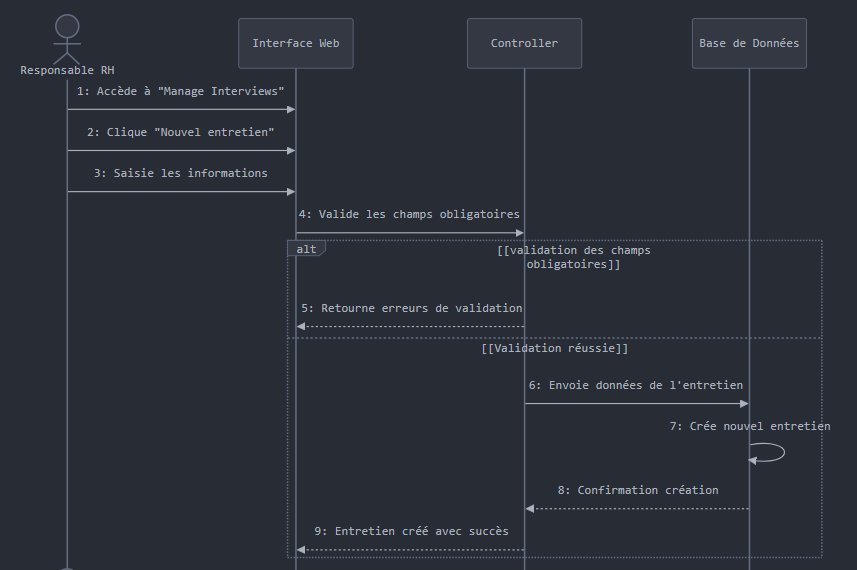
\includegraphics[width=18cm, height=18cm]{Figures/seq3.png}
    \caption{Diagramme de séquence détaillé  au scénario Gestion des entretiens»}

\end{figure}

\section{Réalisation: interfaces Utilisateur dans RhNova }
Dans ce qui suit, nous présentons l’interface dédiée à la gestion des entretiens, qui permet au responsable RH de planifier, modifier ou consulter les entretiens organisés avec les candidats de manière intuitive et structurée.


\vspace{5mm}
\begin{itemize}
     \begin{itemize}
      \item \textbf{Gestion des entretiens  : }Cette interface permet au responsable RH de planifier et gérer les entretiens. Il peut sélectionner la candidature concernée, définir la date, l’heure, la durée, le type d’entretien, son statut, ainsi que préciser le lieu, le lien de meet et les objectifs à évaluer.

         \begin{figure}[H]
             \centering
             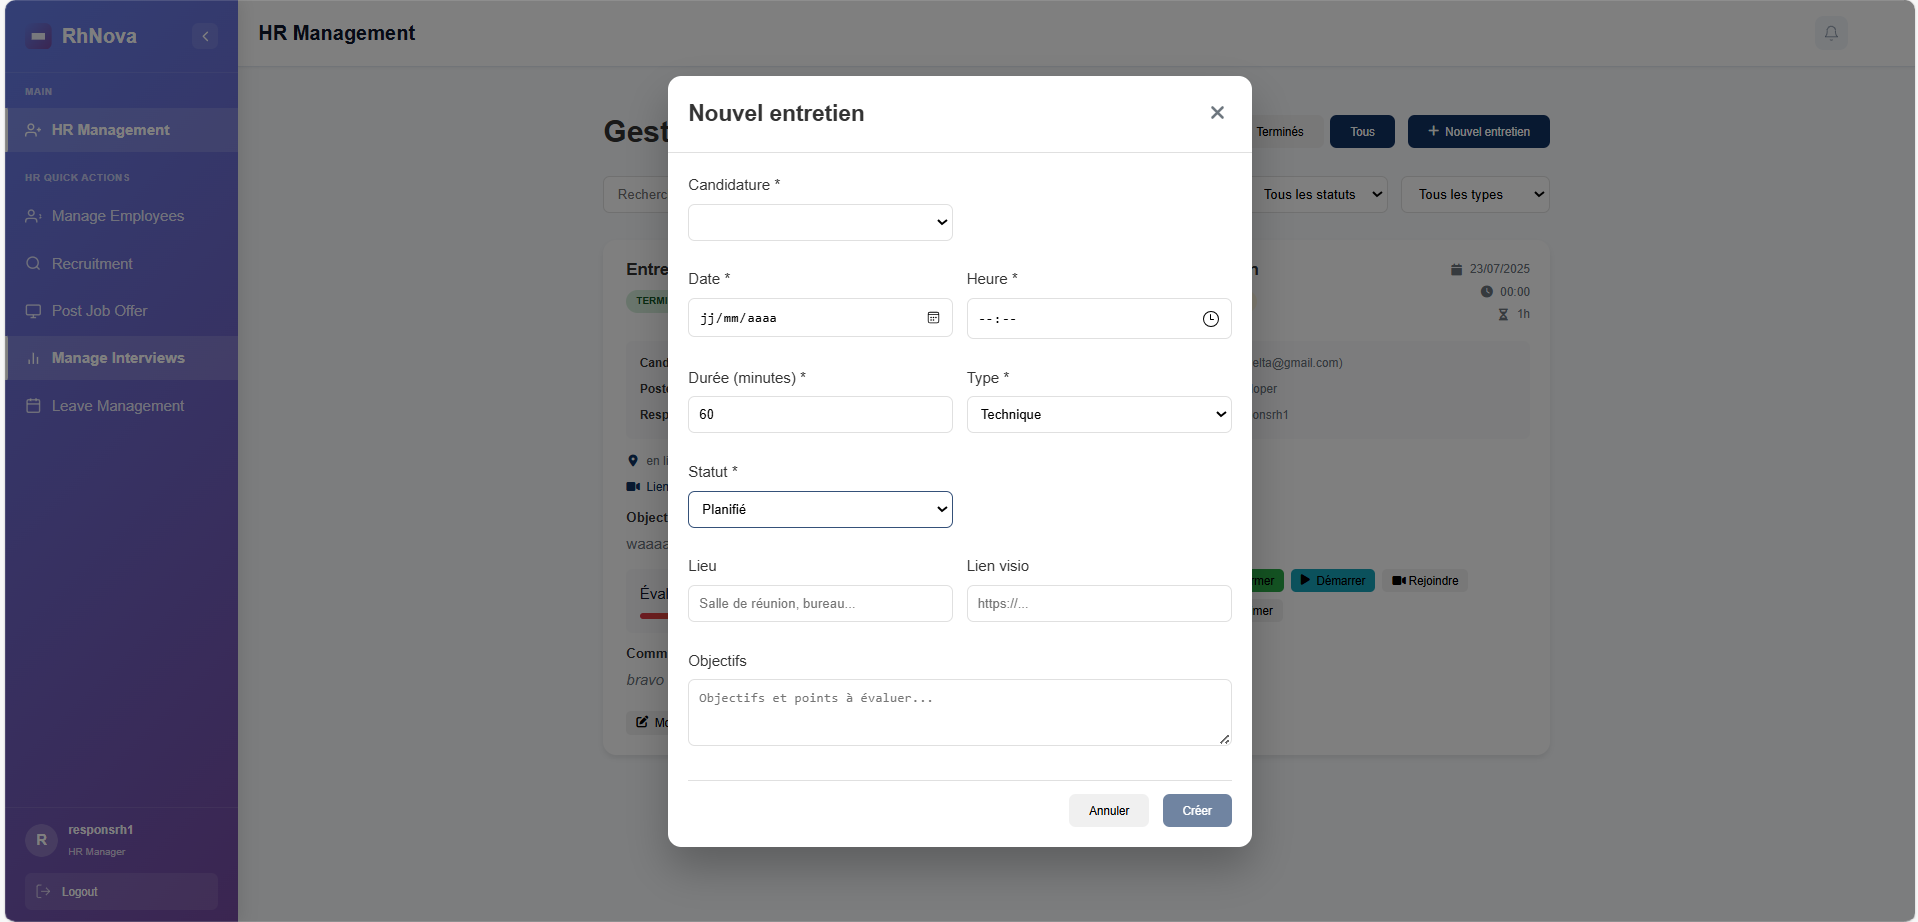
\includegraphics[width=\textwidth]{Figures/responsentretien.png}
             \caption{Liste des connecteurs}
         \end{figure}
     \end{itemize}
\end{itemize}

\section*{Conclusion}
En conclusion, ce chapitre a structuré la Sprint Gestion des Entretiens et ATS, en définissant les objectifs et détaillant le backlog, tout en exposant les diagrammes de cas d’utilisation, classes et de séquences. Les descriptions textuelles et captures d’écran ont confirmé la mise en œuvre réussie, établissant une base solide pour l’optimisation des processus de recrutement. Dans le chapitre suivant, nous aborderons les détails du quatrième  sprint " Gestion des Projets et Équipes".
\addcontentsline{toc}{section}{\protect\numberline{}Conclusion}%


\chead{CHAPITRE 6 . SPRINT 4:Gestion des Projets et Équipes}
 
\chapter{Sprint 4: Gestion des Projets et Équipes}
\renewcommand{\mtctitle}{Sommaire}
\minitoc
\newpage
\section*{Introduction}
\addcontentsline{toc}{section}{\protect\numberline{}Introduction}%
Ce chapitre explore les étapes de la Sprint Gestion des Projets et Équipes, avec un accent particulier sur la structuration des projets, la gestion des équipes et des tâches. Nous débuterons par un aperçu du backlog, avant de détailler la conception, la mise en œuvre et d’illustrer le travail effectué à l’aide de captures d’écran.
\section{Objectifs du Sprint}
L’objectif de cette sprint est de permettre au manager de structurer les projets, gérer les équipes, attribuer des tâches, évaluer les performances, et administrer les fichiers liés aux projets.



\section{Spécification des besoins}
\par Dans cette section, nous allons débuter par présenter le diagramme de cas d’utilisation de la sprint, suivi de l’exposition du backlog associé.
\subsection{Diagramme cas d’utilisation du Sprint 4}

 \begin{figure}[H]
    \centering
    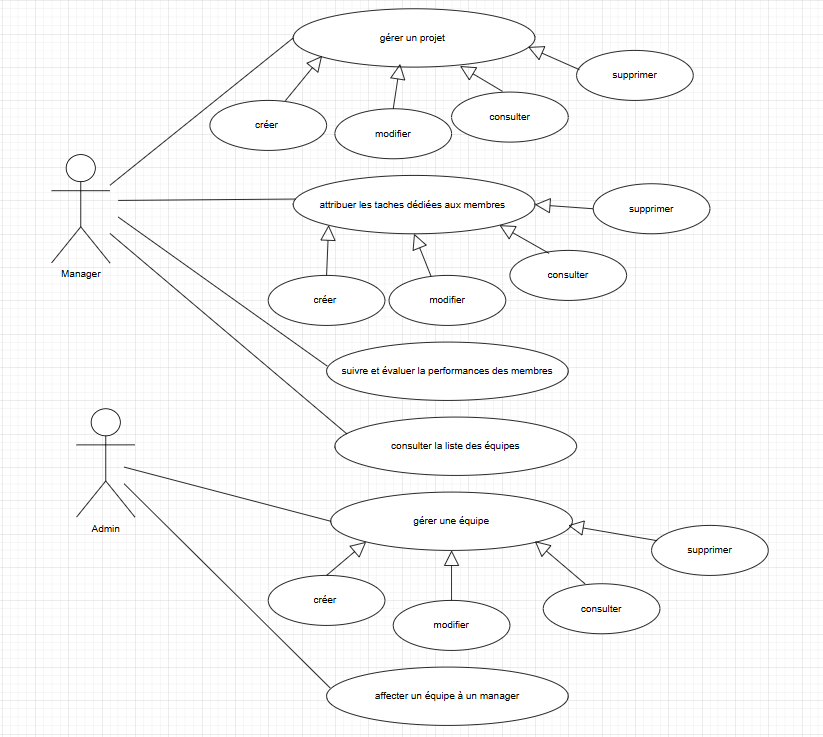
\includegraphics[width=15cm, height=12cm]{Figures/use case 4.png}
    \caption{Diagramme de cas d’utilisation du sprint 4}
    \label{fig:Diagramme de cas d’utilisation du sprint 0}
\end{figure}

\subsection{ Sprint Backlog du sprint 4}
Le tableau ci-dessous présente le sprint backlog établi pour le quatrième sprint. Il récapitule les différentes user stories sélectionnées, accompagnées de leurs identifiants uniques, ainsi que les tâches techniques à réaliser pour chacune. Ce tableau permet d’avoir une vision claire et structurée du travail prévu, en facilitant la planification, la répartition des responsabilités et le suivi de l’avancement tout au long du sprint.
\textbf{\begin{table}[H]
\caption{Backlog du sprint 4}
\centering
\begin{tabular}{|p{1cm}|p{8cm}|p{8cm}|}
\hline
\textbf{ID} & \textbf{User Story} & \textbf{Tâches techniques} \\
\hline
US-17 & En tant que manager, je veux créer, modifier, supprimer des projets afin de structurer mon équipe. 
& 
\begin{itemize}[leftmargin=*]
  \item Concevoir le modèle de données pour les projets.
  \item Créer des interfaces de gestion CRUD.
  \item Implémenter la logique de gestion des projets.
\end{itemize} \\
\hline
US-18 & En tant qu’administrateur, je veux créer, modifier, supprimer une équipe. 
& 
\begin{itemize}[leftmargin=*]
  \item Définir le modèle "Équipe".
  \item Créer les interfaces de gestion.
  \item Gérer les interactions avec la base de données.
\end{itemize} \\
\hline
US-19 & En tant qu’administrateur, je veux affecter une équipe à un manager. 
& 
\begin{itemize}[leftmargin=*]
  \item Ajouter une relation entre équipe et manager.
  \item Enregistrer l'affectation dans la base.
\end{itemize} \\
\hline
US-20 & En tant que manager, je peux consulter les équipes affectées par l’administrateur. 
& 
\begin{itemize}[leftmargin=*]
  \item Développer une interface de visualisation des équipes.
  \item Mettre en place une requête filtrée par manager.
  \item Afficher les données de manière claire.
\end{itemize} \\
\hline
US-21 & En tant que manager, je veux attribuer des tâches aux membres de mon équipe. 
& 
\begin{itemize}[leftmargin=*]
  \item Créer un formulaire d'attribution de tâche.
  \item Lier une tâche à un membre de l’équipe.
  \item Enregistrer l'information dans la base.
\end{itemize} \\
\hline
US-22 & En tant que manager, je veux évaluer la progression des tâches réalisées par les membres de mon équipe. 
& 
\begin{itemize}[leftmargin=*]
  \item Ajouter un champ "état/avancement" dans le modèle tâche.
  \item Créer un tableau de suivi des tâches par membre.
  \item Générer un affichage visuel (ex. barre de progression).
\end{itemize} \\
\hline
\end{tabular}
\label{tab:sprint4_backlog}
\end{table}
}





\section{Analyse des besoins}
Avant de modéliser les fonctionnalités du système, il est essentiel de comprendre les besoins fonctionnels exprimés à travers les différents cas d’usage. La section suivante propose une description textuelle de ces cas d’utilisation, permettant de mieux cerner les interactions entre les utilisateurs et le système, et de poser les bases d’une modélisation cohérente.
    
\subsection{Description textuelle de cas d'utilisation}
   
     \item \textbf{Cas d'utilisation "Gérer un projet": } La table 6.2 ci-dessous présente la description textuelle du cas d'utilisation « Gérer un projet ».

 \begin{table}[H]
 \caption{ Description textuelle du cas d’utilisation "Gérer un projet"}
    \centering
    \begin{tabular}{|c|p{12cm}|}
    \hline
    \textbf{Titre} & Gérer un projet \\
    \hline
    \textbf{Objectif} & Permettre au manager de créer, modifier, supprimer et consulter des projets pour structurer son équipe. \\
    \hline
    \textbf{Acteur}& Manager\\
    \hline
    \textbf{Pré-condition} &Le manager doit être authentifié et avoir les droits d’accès nécessaires.
    \\
    \hline
    \textbf{Post-condition} &Les modifications ou suppressions des projets sont enregistrées dans le système.\\
    \hline
    \textbf{Scénario nominal} & 1. Le manager accède à l’interface de gestion des projets.\newline
    2. Il sélectionne une action (créer, modifier, supprimer).\newline
    3. Il entre ou modifie les détails du projet (nom, description).\newline
    4. Le système valide et enregistre les changements.
    \\
    \hline
    \end{tabular}
    \label{tab:user_stories}
\end{table}

      \item \textbf{Cas d'utilisation "Gérer une équipe": } La table 6.3 ci-dessous présente la description textuelle du cas d'utilisation « Gérer une équipe ».
 \begin{table}[H]
  \caption{ Description textuelle du cas d’utilisation "tableau de bord"}
    \centering
    \begin{tabular}{|c|p{12cm}|}
    \hline
    \textbf{Titre} & Gérer une équipe \\
    \hline
    \textbf{Objectif} & Permettre au manager de créer, modifier, supprimer et consulter des équipes. \\
    \hline
    \textbf{Acteur}& Admin\\
    \hline
    \textbf{Pré-condition} & L'admin doit être authentifié.
    \\
    \hline
    \textbf{Post-condition} & Les modifications ou suppressions des équipes sont enregistrées dans le système.\\
    \hline
    \textbf{Scénario nominal} & 1. L'admin accède à la gestion des équipes. \newline
    2. Il choisit une action (créer, modifier, supprimer).\newline
    3. Il entre les détails (nom de l’équipe, membres, ect.).
    \newline
    4.Le système enregistre les données.\\
    \hline
    \end{tabular}
    \label{tab:user_stories}
\end{table}

      \item \textbf{Cas d'utilisation "Attribuer les tâches aux membres": } La table 6.4 ci-dessous présente la description textuelle du cas d'utilisation « Attribuer les tâches aux membres ».
 \begin{table}[H]
 \caption{ Description textuelle du cas d’utilisation "Attribuer les tâches aux membres"}
    \centering
    \begin{tabular}{|c|p{12cm}|}
    \hline
    \textbf{Titre} & Attribuer les tâches aux membres \\
    \hline
    \textbf{Objectif} & Permettre au manager d’assigner des tâches spécifiques aux membres de son équipe. \\
    \hline
    \textbf{Acteur}& Manager\\
    \hline
    \textbf{Pré-condition} & Une équipe et des tâches doivent exister dans le système.
    \\
    \hline
    \textbf{Post-condition} & Les tâches sont attribuées et visibles pour les membres concernés.\\
    \hline
    \textbf{Scénario nominal} & 1. Le manager accède à la gestion des tâches. \newline
    2. Il sélectionne une tâche et un membre.\newline
    3. Il confirme l’attribution.\newline
    4. Le système met à jour l’assignation.\\
    \hline
    \end{tabular}
    \label{tab:user_stories}
\end{table}

      \item \textbf{Cas d'utilisation "Suivre et évaluer la performance des membres": } La table 6.5 ci-dessous présente la description textuelle du cas d'utilisation « Suivre et évaluer la performance des membres ».
 \begin{table}[H]
 \caption{ Description textuelle du cas d’utilisation "Suivre et évaluer la performance des membres"}
    \centering
    \begin{tabular}{|c|p{12cm}|}
    \hline
    \textbf{Titre} & Suivre et évaluer la performance des membres\\
    \hline
    \textbf{Objectif} & Permettre au manager de surveiller et évaluer la performance des membres de son équipe.. \\
    \hline
    \textbf{Acteur}& Manager\\
    \hline
    \textbf{Pré-condition} & Les membres doivent avoir des tâches assignées.
    \\
    \hline
    \textbf{Post-condition} & L’évaluation est enregistrée et accessible pour consultation.\\
    \hline
    \textbf{Scénario nominal} & 1. Le manager accède à l’interface de suivi. \newline
    2. Il permet de consulter la liste des tâches.\newline
    3. limite l’évaluation aux observations sur le progrès des tâches\\
    \hline
    \end{tabular}
    \label{tab:user_stories}
\end{table}

     \item \textbf{Cas d'utilisation "Affecter une équipe à un manager": } La table 6.6 ci-dessous présente la description textuelle du cas d'utilisation « Affecter une équipe à un managers ».
 \begin{table}[H]
 \caption{ Description textuelle du cas d’utilisation "Affecter une équipe à un manager"}
    \centering
    \begin{tabular}{|c|p{12cm}|}
    \hline
    \textbf{Titre} & Affecter une équipe à un manager\\
    \hline
    \textbf{Objectif} & Permettre à l’administrateur d’affecter un manager à une équipe lors de sa création. \\
    \hline
    \textbf{Acteur}& Administrateur\\
    \hline
    \textbf{Pré-condition} & L’administrateur doit être authentifié et un manager doit être disponible dans le système.
    \\
    \hline
    \textbf{Post-condition} & L’équipe est créée avec le manager assigné et les informations sont enregistrées.\\
    \hline
    \textbf{Scénario nominal} & 1. L’administrateur accède à l’interface de gestion des équipes. \newline
    2. Il crée une nouvelle équipe en entrant les détails (nom, description).\newline
    3. Il sélectionne un manager à affecter à l’équipe.\newline
    4. Le système enregistre l’équipe avec le manager assigné.\\
    \hline
    \end{tabular}
    \label{tab:user_stories}
\end{table}
 
\section{Conception}
\hspace{0.5cm}\textbf Dans cette section, nous discutons de la conception du quatrième sprint. nous Commençons par le diagramme de classes du sprint. Ensuite, nous examinons la modélisation de quelques diagrammes de séquences .  


\subsection{Diagrammes de séquences}
Dans le cadre de l’analyse dynamique du système, un diagramme de séquence a été réalisé pour chaque fonctionnalité clé développée lors des sprints. Le diagramme ci-dessous illustre spécifiquement le scénario du cas d'utilisation « Gérer une équipe », permettant de visualiser les interactions entre l'administrateur et le système lors de la création d’une nouvelle équipe.

\subsubsection{Diagramme de séquence  au cas d’utilisation «Gérer une équipe»}

Cette figure illustre le déroulement du scénario associé à ce cas d'utilisation.
     \begin{figure}[H]
    \centering
    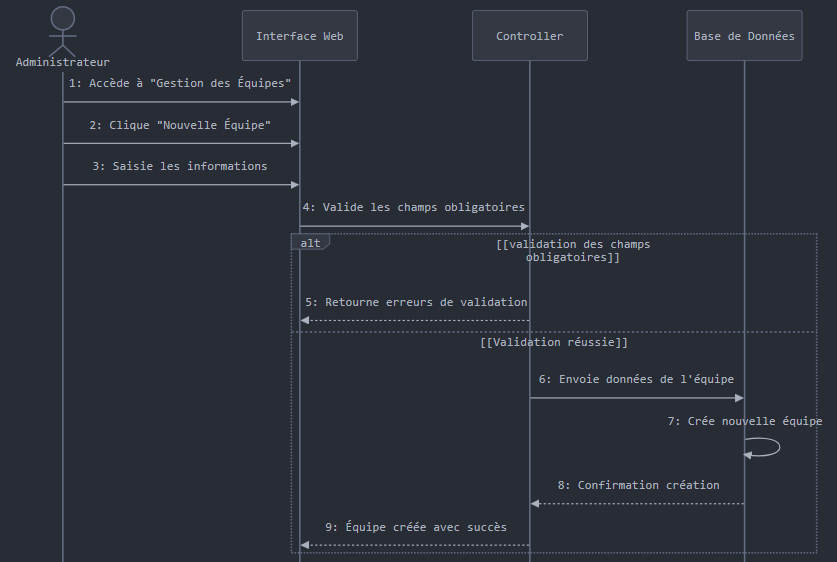
\includegraphics[width=18cm, height=23cm]{Figures/seq4.png}
    \caption{Diagramme de séquence  au scénario « Gérer une équipe »}

\end{figure}

\section{Réalisation: interfaces utilisateur dans HrNova }
CLes interfaces développées dans le cadre de ce sprint permettent aux managers et administrateurs de gérer efficacement les projets, les équipes et les tâches associées. Elles offrent une vue claire sur l’organisation du travail, le suivi des objectifs et la répartition des rôles au sein des équipes.

\vspace{5mm}
\begin{itemize}
     \begin{itemize}
      \item \textbf{Gestion des projets: } Cette interface permet au manager de suivre et gérer les projets. Il peut visualiser la liste des projets, leur statut, leur avancement en pourcentage, ainsi que consulter et modifier les détails de chaque projet, attribuer des équipes et gérer les échéances.
         \begin{figure}[H]
             \centering
             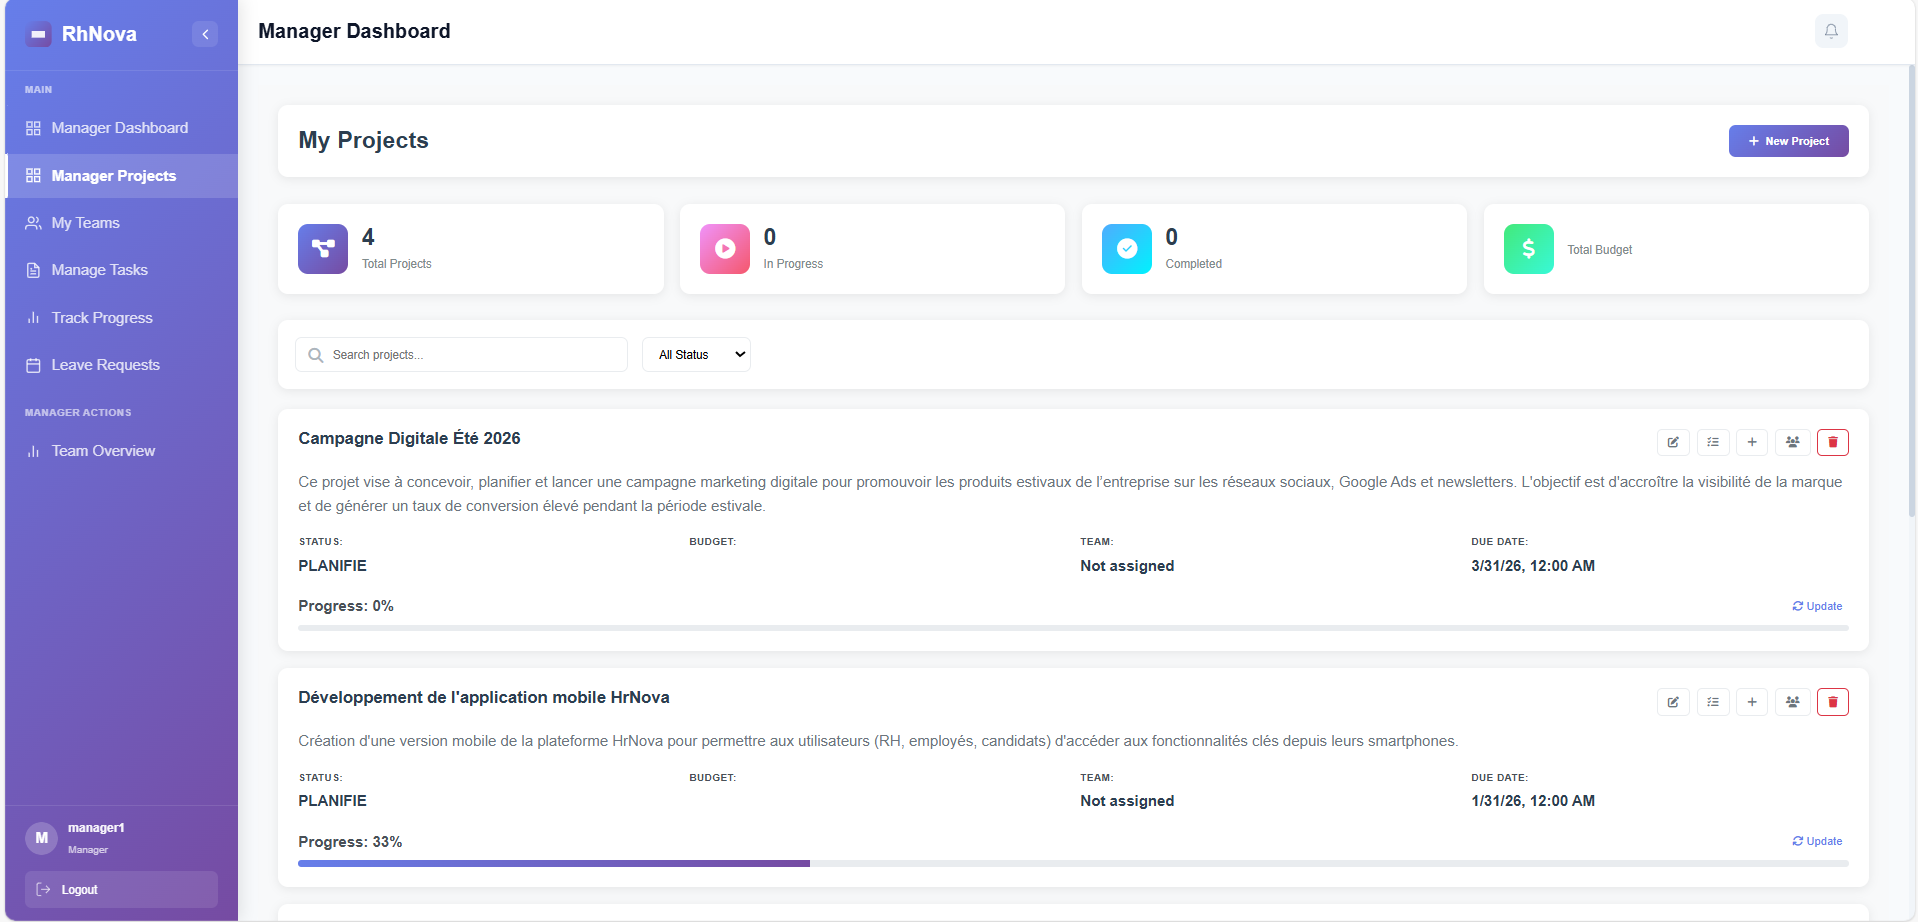
\includegraphics[width=\textwidth]{Figures/managerprojet.png}
             \caption{Page de gestion de projet}
         \end{figure}
     \end{itemize}
\end{itemize}
\begin{itemize}
     \item\textbf{Gestion des tâches : }
Cette interface permet au manager de créer, gérer et suivre les tâches liées aux projets. Il peut définir les priorités, affecter les tâches aux membres de l’équipe, fixer des dates d’échéance, et suivre l’avancement de chaque tâche.
         \begin{figure}[H]
             \centering
             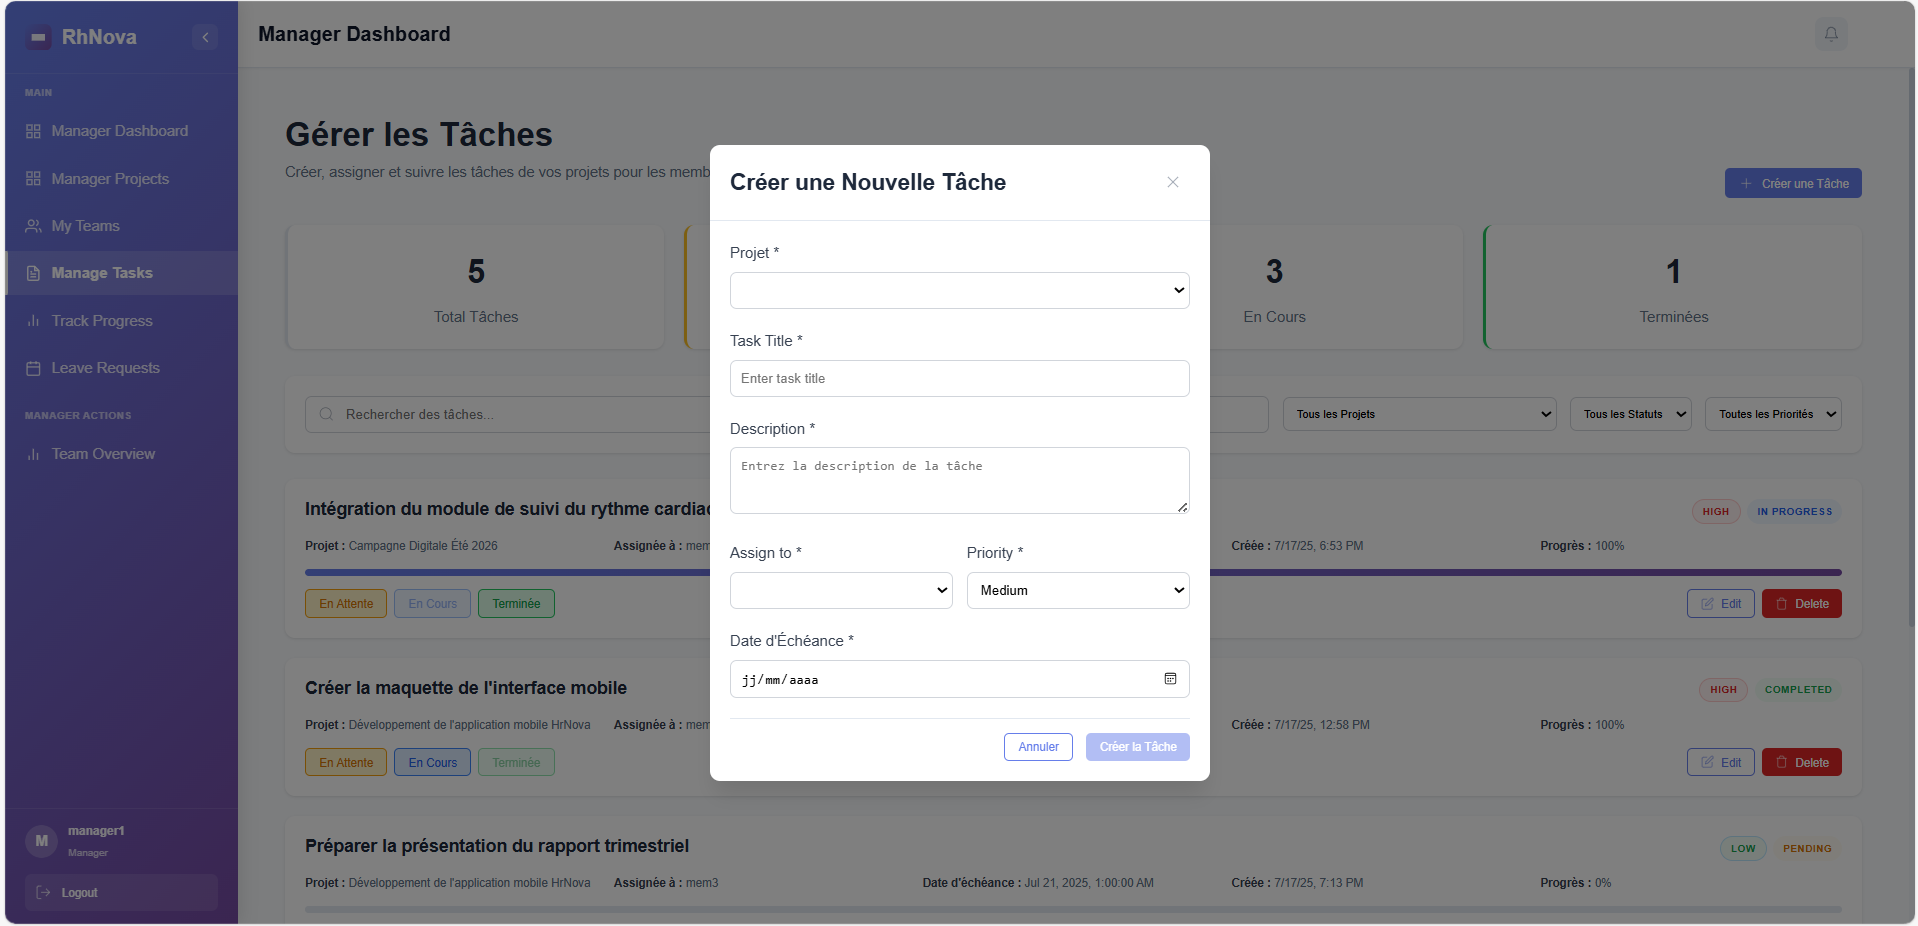
\includegraphics[width=\textwidth]{Figures/managertache.png}
             \caption{Page de gestion des tâches }
         \end{figure}
\end{itemize}  
\begin{itemize}
 \item\textbf{Suivi de la progression : }
Cette interface permet au manager d’évaluer et afin de visualiser l’avancement en direct des tâches assignées aux membres de l’équipe. Elle affiche des indicateurs de performance tels que le nombre de tâches terminées, en cours et en retard, ainsi que le taux de réussite global. Un tableau détaillé liste chaque tâche avec son avancement, sa priorité, son statut, son échéance et le temps passé.
         \begin{figure}[H]
             \centering
             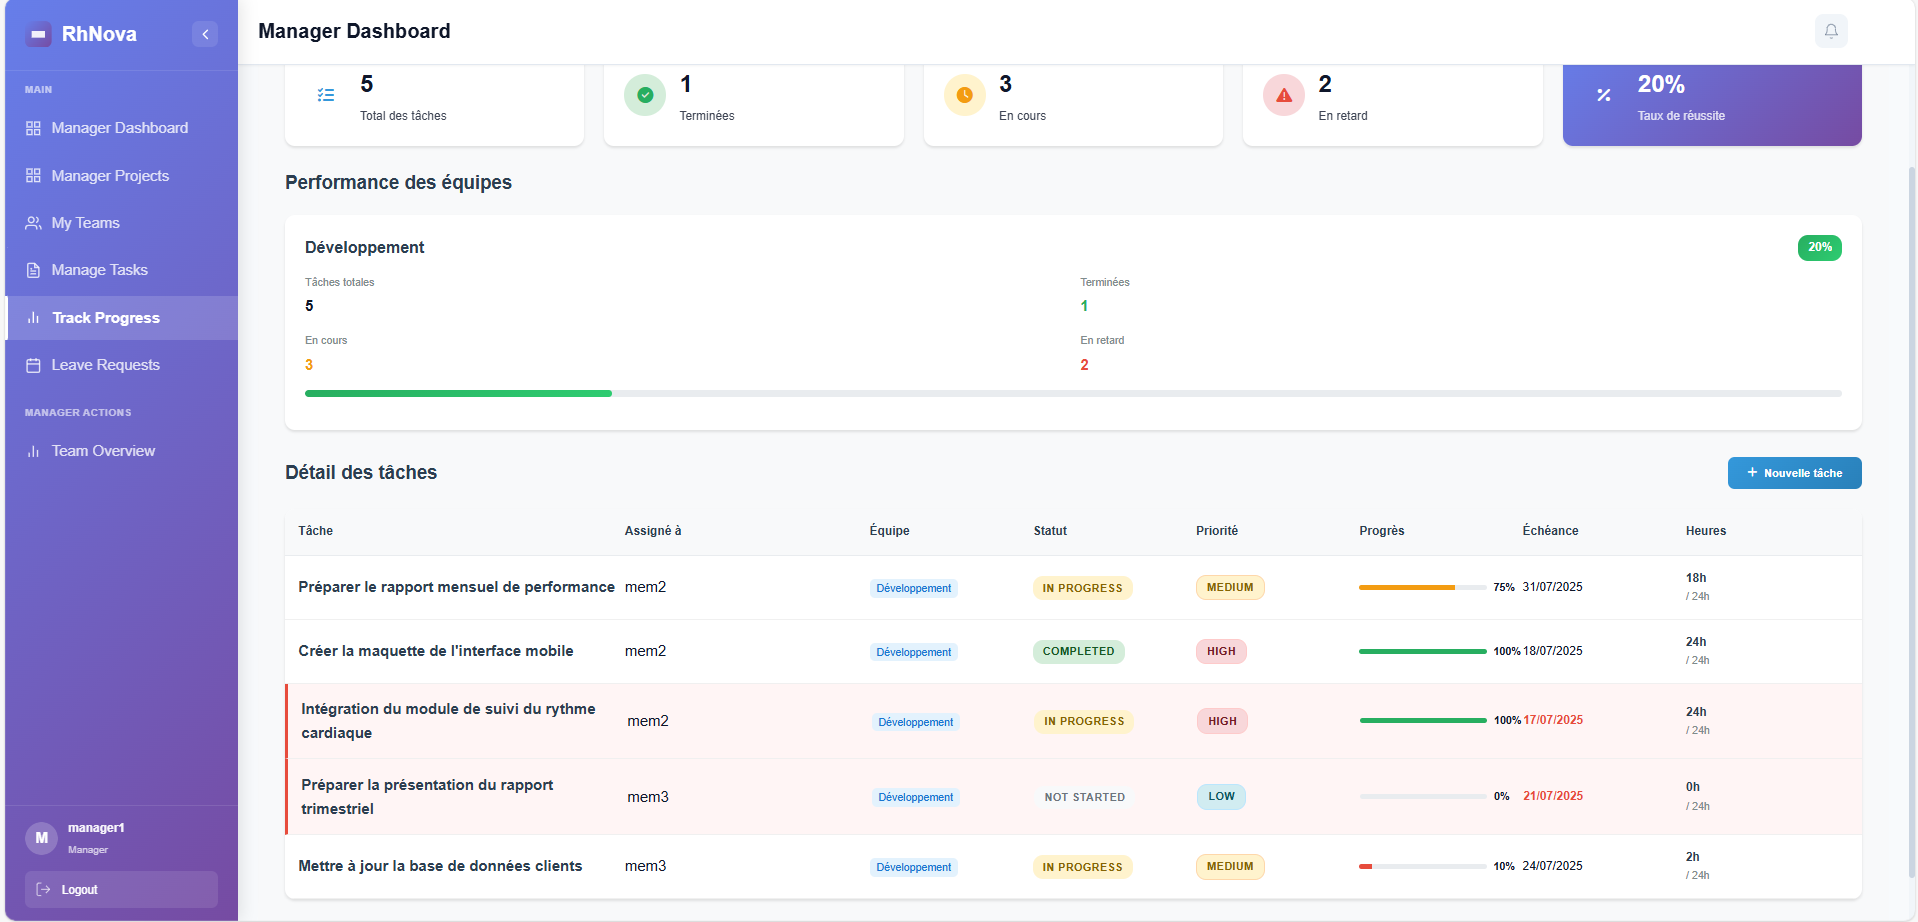
\includegraphics[width=\textwidth]{Figures/managerevalu.png}
             \caption{Page suivi de progression}
         \end{figure}

     \end{itemize}
\begin{itemize}
         \item \textbf{Consultation des équipes : } Cette interface permet au manager de consulter la composition des équipes qui lui ont été attribuées par l’administrateur. 
         \begin{figure}[H]
             \centering
             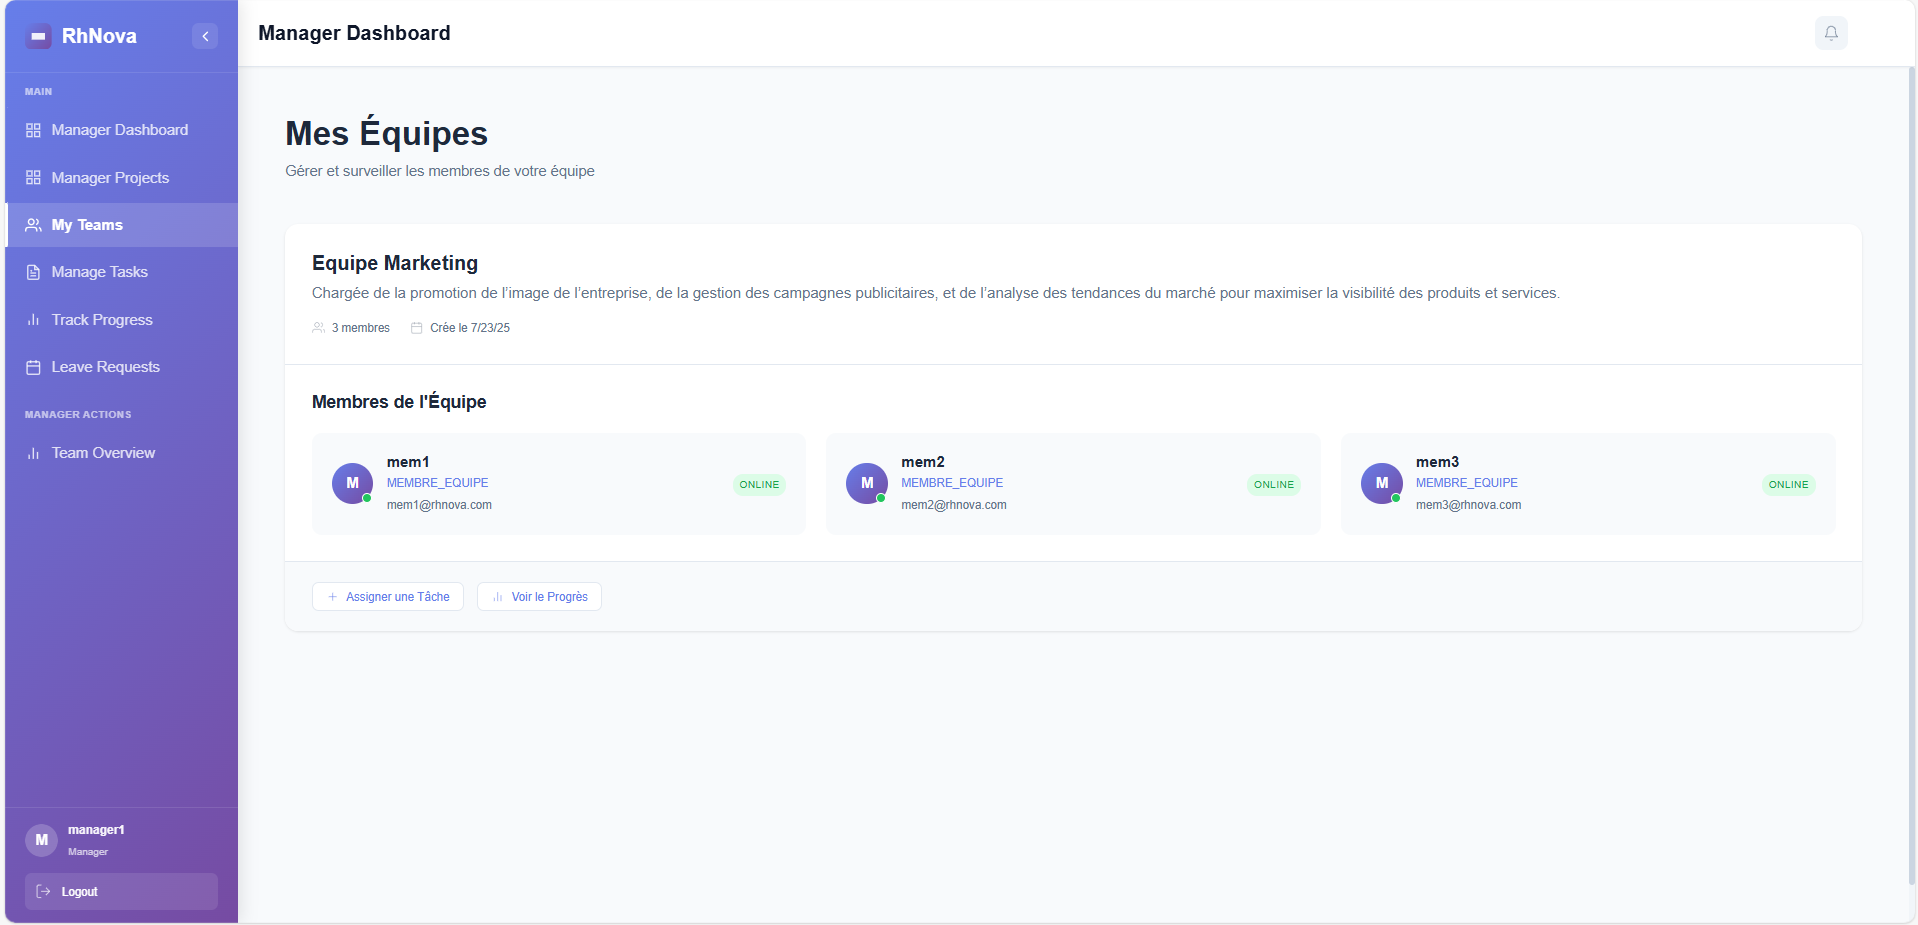
\includegraphics[width=\textwidth]{Figures/managerequipe.png}
             \caption{Page consultation des équipes }
         \end{figure}
     \end{itemize}
\begin{itemize}
         \item \textbf{Gestion des Équipes  : } Cette interface de gestion des équipes est dédiée à l’administrateur. Elle lui permet de créer de nouvelles équipes en renseignant le nom, le manager responsable et une description. 
         \begin{figure}[H]
             \centering
             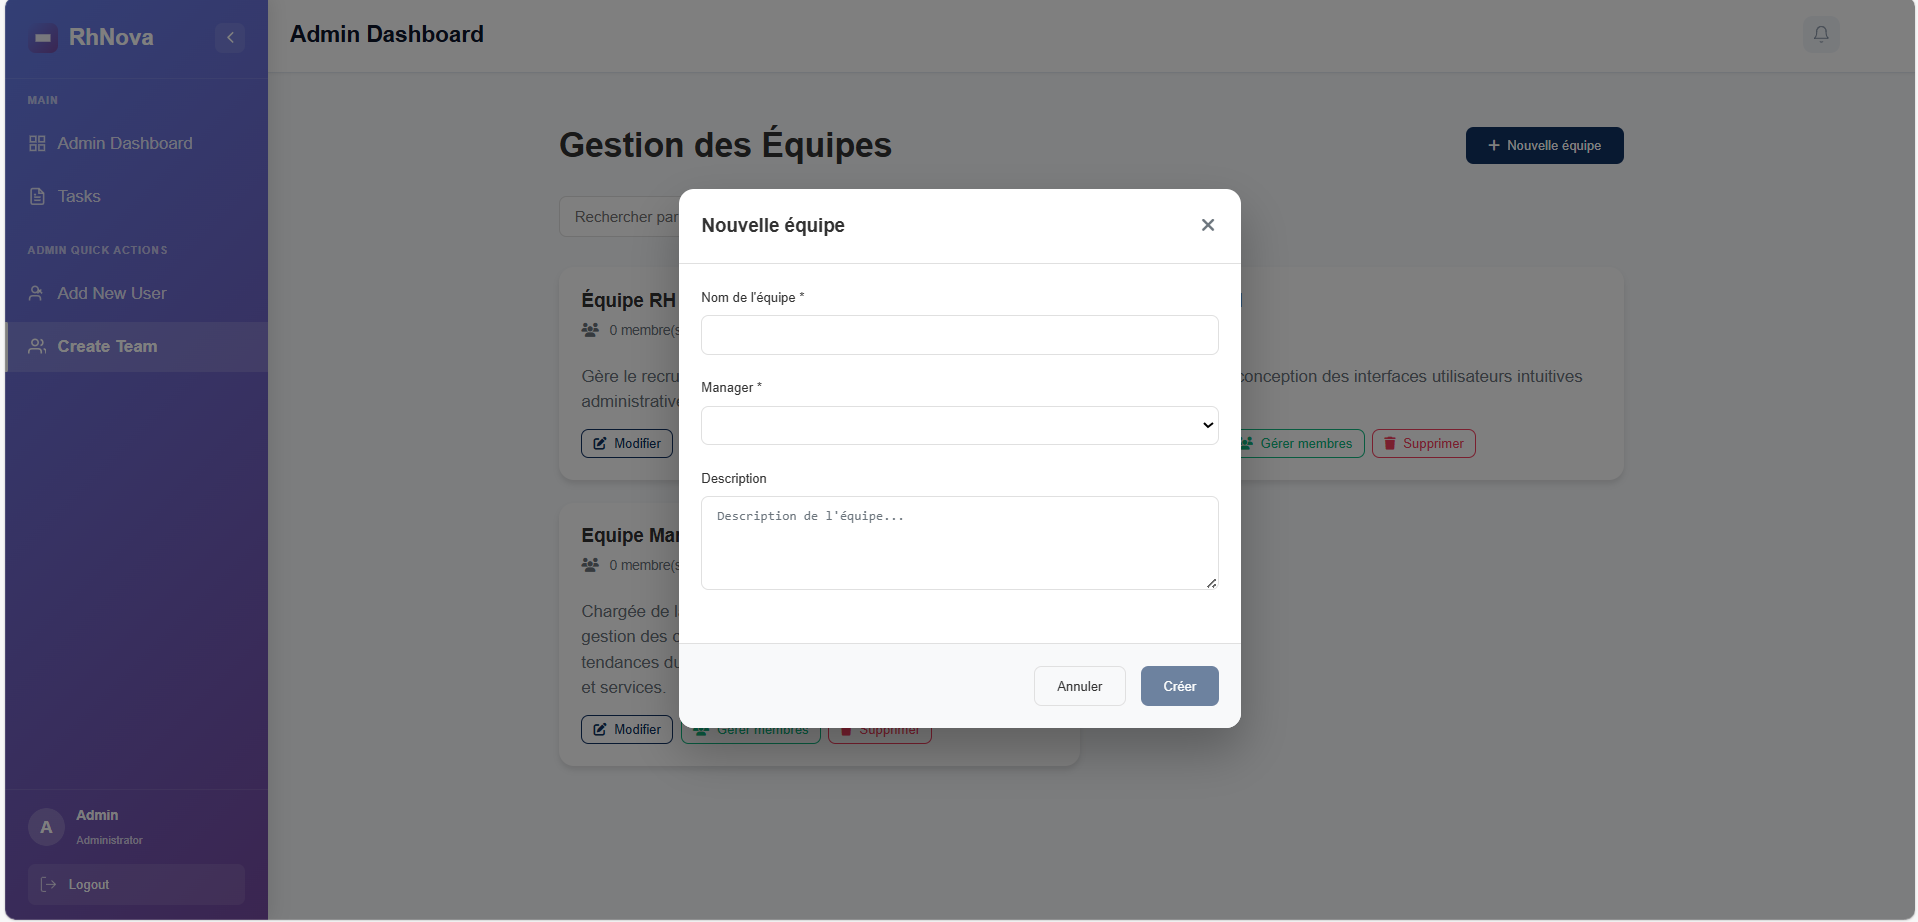
\includegraphics[width=\textwidth]{Figures/admingenerteam.png}
             \caption{Page de gestion des équipes}
         \end{figure}
     \end{itemize}

\section*{Conclusion}
En conclusion, ce chapitre a structuré la Sprint Gestion des Projets & Équipes, en définissant les objectifs et détaillant le backlog, tout en exposant les diagrammes de cas d’utilisation et de classes. Les descriptions textuelles et captures d’écran ont confirmé la mise en œuvre réussie, établissant une base solide pour la gestion des équipes et des projets à venir. Dans le chapitre suivant, nous aborderons les détails du quatrième  sprint " Gestion des Congés et Tâches".
\addcontentsline{toc}{section}{\protect\numberline{}Conclusion}%
\chead{CHAPITRE 7. SPRINT 5 : Gestion des Congés et Tâches}

\chapter{Sprint 5: Gestion des Congés et Tâches}
\renewcommand{\mtctitle}{Sommaire}
\minitoc
\newpage
\section*{Introduction}
\addcontentsline{toc}{section}{\protect\numberline{}Introduction}%
Ce chapitre explore les étapes de la Sprint Gestion des Congés et Tâches, avec un accent particulier sur la gestion des demandes de congé et la supervision des tâches. Nous débuterons par un aperçu du backlog, avant de détailler la conception, la mise en œuvre et d’illustrer le travail effectué à l’aide de captures d’écran.

\section{Objectifs du Sprint}
L’objectif de cette sprint est de permettre la soumission et la validation des demandes de congé, la consultation et la gestion des tâches par les membres d’équipe, ainsi que la création de rapports de travail pour documenter l’avancement.

\section{Spécification des besoins}
\par Dans cette section, nous commencerons par présenter le diagramme des cas d’utilisation du sprint, puis nous exposerons le backlog associé.
\subsection{Diagramme cas d'utlisation du sprint 5}

\begin{figure}[H]
\centering
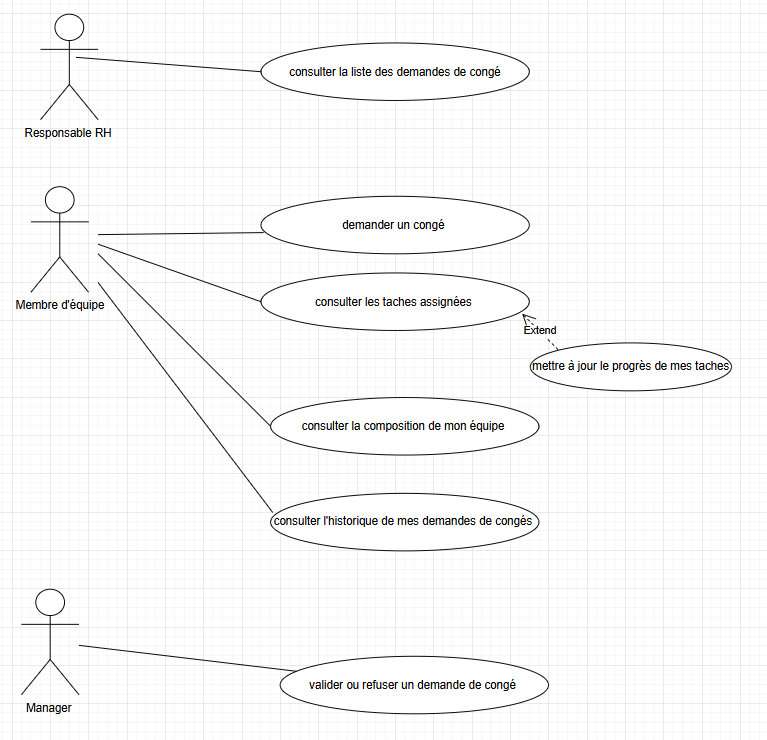
\includegraphics[width=15cm, height=12cm]{Figures/use case 5.png}
\caption{Diagramme de cas d’utilisation du Sprint 5}
\label{schema1}
\end{figure}

\subsection{ Sprint Backlog du sprint 5}
Le tableau ci-dessous présente le sprint backlog établi pour le cinquième sprint. Il récapitule les différentes user stories sélectionnées, accompagnées de leurs identifiants uniques, ainsi que les tâches techniques à réaliser pour chacune. Ce tableau permet d’avoir une vision claire et structurée du travail prévu, en facilitant la planification, la répartition des responsabilités et le suivi de l’avancement tout au long du sprint.
\begin{table}[H]
\caption{Backlog du sprint 5}
\centering
\begin{tabular}{|p{1cm}|p{8cm}|p{8cm}|}
\hline
\textbf{ID} & \textbf{User Story} & \textbf{Tâches techniques} \\
\hline
US-23 & En tant que membre d’équipe, je veux faire une demande de congé. 
& 
\begin{itemize}[leftmargin=*]
  \item Créer un formulaire de demande de congé.
  \item Valider les champs et enregistrer la demande.
  \item Sauvegarder la demande dans la base.
\end{itemize} \\
\hline
US-24 & En tant que manager, je veux valider ou refuser les demandes de congé des membres de mon équipe. 
& 
\begin{itemize}[leftmargin=*]
  \item Lister les demandes en attente.
  \item Ajouter les boutons d'approbation/refus.
  \item Mettre à jour le statut de la demande.
\end{itemize} \\
\hline
US-25 & En tant que responsable RH, je veux consulter la liste des demandes de congé. 
& 
\begin{itemize}[leftmargin=*]
  \item Concevoir l’interface d’affichage.
  \item Afficher toutes les demandes avec leurs statuts.
  \item Implémenter le tri et filtrage par statut.
\end{itemize} \\
\hline
US-26 & En tant que membre d’équipe, je veux consulter les tâches assignées. 
& 
\begin{itemize}[leftmargin=*]
  \item Créer une vue "mes tâches".
  \item Lier les tâches à l'utilisateur connecté.
  \item Afficher les tâches par priorité ou date.
\end{itemize} \\
\hline
US-27 & En tant que membre d’équipe, je veux consulter la composition de mon équipe. 
& 
\begin{itemize}[leftmargin=*]
  \item Ajouter une relation membre-équipe.
  \item Développer une interface de visualisation.
  \item Afficher la liste des membres de l’équipe.
\end{itemize} \\
\hline
US-28 & En tant que membre d’équipe, je veux mettre à jour le progrès de mes tâches. 
& 
\begin{itemize}[leftmargin=*]
  \item Ajouter un champ de progression dans chaque tâche.
  \item Enregistrer les modifications dans la base.
\end{itemize} \\
\hline
US-29 & En tant que membre d’équipe, je veux consulter l’historique de mes demandes de congés. 
& 
\begin{itemize}[leftmargin=*]
  \item Lister toutes les demandes de l'utilisateur.
  \item Ajouter une section historique avec filtre.
  \item Afficher les statuts de chaque demande.
\end{itemize} \\
\hline
\end{tabular}
\label{tab:sprint5_backlog}
\end{table}


\section{Analyse des besoins}
Avant de modéliser les fonctionnalités du système, il est essentiel de comprendre les besoins fonctionnels exprimés à travers les différents cas d’usage. La section suivante propose une description textuelle de ces cas d’utilisation, permettant de mieux cerner les interactions entre les utilisateurs et le système, et de poser les bases d’une modélisation cohérente.
    
\subsection{description textuelle de cas d'utilisation}

     \item \textbf{Cas d'utilisation "Valider ou refuser une demande de congé": } La table 7.2 ci-dessous présente la description textuelle du cas d'utilisation « Valider ou refuser une demande de congé ».

 \begin{table}[H]
 \caption{ Description textuelle du cas d’utilisation "Valider ou refuser une demande de congé"}
    \centering
    \begin{tabular}{|c|p{12cm}|}
    \hline
    \textbf{Titre} & Valider ou refuser une demande de congé \\
    \hline
    \textbf{Objectif} & Permettre au manager d’accepter ou refuser une demande de congé d’un membre d’équipe. \\
    \hline
    \textbf{Acteur}& Manager\\
    \hline
    \textbf{Pré-condition} & Une demande de congé doit avoir été soumise par un membre d’équipe et le manager doit être authentifié.
    \\
    \hline
    \textbf{Post-condition} & La décision (acceptation ou refus) est enregistrée et notifiée au membre d’équipe.\\
    \hline
    \textbf{Scénario nominal} & 1. Le manager accède à la liste des demandes de congé. \newline
    2. Il sélectionne une demande.\newline
    3. Il choisit d’accepter ou de refuser la demande.
    \newline
    4. Le système enregistre la décision.\\
    \hline
    \end{tabular}
    \label{tab:user_stories}
\end{table}


     \item \textbf{Cas d'utilisation "Demander un congé": } La table 7.3 ci-dessous présente la description textuelle du cas d'utilisation « Demander un congé ».

 \begin{table}[H]
 \caption{ Description textuelle du cas d’utilisation "Demander un congé"}
    \centering
    \begin{tabular}{|c|p{12cm}|}
    \hline
    \textbf{Titre} & Demander un congé \\
    \hline
    \textbf{Objectif} & Permettre au membre d’équipe de soumettre une demande de congé à son manager. \\
    \hline
    \textbf{Acteur}& Membre d’équipe\\
    \hline
    \textbf{Pré-condition} & Le membre d’équipe doit être authentifié et avoir un manager assigné.\\
    \hline
    \textbf{Post-condition} & La demande de congé est soumise et en attente de validation par le manager.\\
    \hline
    \textbf{Scénario nominal} & 1. Le membre d’équipe accède à l’interface de gestion des congés. \newline
    2. Il entre les détails de la demande (dates, motif).\newline
    3. Il soumet la demande au manager.
    \newline
    4. Le système enregistre la demande en attente de validation.
    \\
    \hline
    \end{tabular}
    \label{tab:user_stories}
\end{table}

     \item \textbf{Cas d'utilisation "Consulter les tâches": } La table 7.4 ci-dessous présente la description textuelle du cas d'utilisation « Consulter les tâches ».

 \begin{table}[H]
 \caption{ Description textuelle du cas d’utilisation "Consulter les tâches"}
    \centering
    \begin{tabular}{|c|p{12cm}|}
    \hline
    \textbf{Titre} & Consulter les tâches \\
    \hline
    \textbf{Objectif} & Permettre au membre d’équipe de visualiser les tâches assignées par le manager. \\
    \hline
    \textbf{Acteur}& Membre d’équipe\\
    \hline
    \textbf{Pré-condition} & Le membre d’équipe doit être authentifié et des tâches doivent lui être assignées par le manager.
    \\
    \hline
    \textbf{Post-condition} & La liste des tâches assignées est affichée avec leurs statuts.\\
    \hline
    \textbf{Scénario nominal} & 1. Le membre d’équipe accède à l’interface de gestion des tâches. \newline
    2. Il sélectionne l’option de consultation.\newline
    3. Le système affiche les tâches assignées par le manager.\newline
    4. Il consulte les détails.\\
    \hline
    \end{tabular}
    \label{tab:user_stories}
\end{table}


   

   

\section{Conception}
\hspace{0.5cm}\textbf Dans cette section, nous discutons de la conception du quatrième sprint. nous Commençons par le diagramme de classes du sprint. Ensuite, nous examinons la modélisation de quelques diagrammes de séquences . 

\subsection{Diagrammes de séquences}
Dans le cadre de l’analyse dynamique du système, un diagramme de séquence a été réalisé pour chaque fonctionnalité clé développée lors des sprints. Le diagramme ci-dessous illustre spécifiquement le scénario du cas d'utilisation « Demander un congé », permettant de visualiser les interactions entre le membre d'équipe et le système lors de la création d’un nouvel demande de congé.

\subsubsection{Diagramme de séquence au cas d’utilisation «Demander un congé»}

Cette figure illustre le déroulement du scénario associé à ce cas d'utilisation.
     \begin{figure}[H]
    \centering
    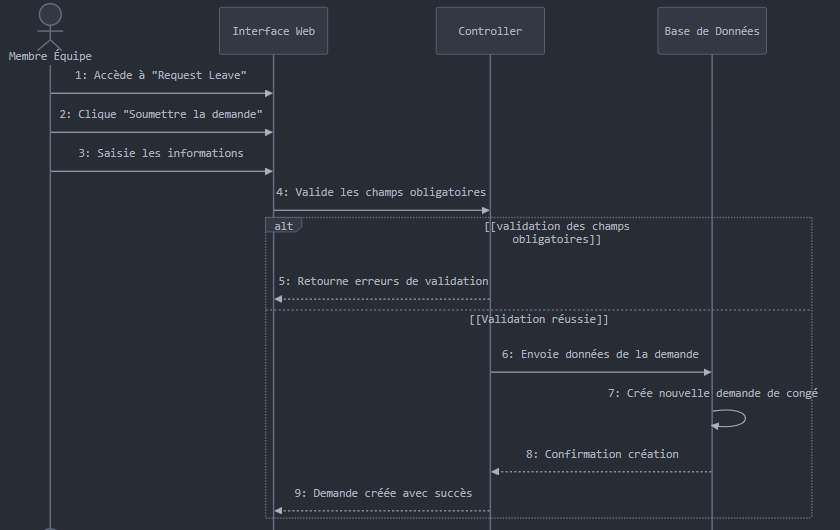
\includegraphics[width=18cm, height=23cm]{Figures/seq5.png}
    \caption{Diagramme de séquence au scénario «Demander un congé»}

\end{figure}

\section{Réalisation: Interfaces Utilisateur dans RhNova}
Dans cette dernière phase du projet, plusieurs interfaces ont été conçues pour faciliter la gestion des congés et des tâches au sein des équipes. Ces interfaces permettent aux utilisateurs de soumettre et suivre leurs demandes de congé, de gérer leurs tâches quotidiennes, et de consulter les informations relatives à leur équipe et à l’historique des congés.

\vspace{5mm}
\begin{itemize}
     \begin{itemize}
      \item \textbf{Suivre demandes de congé: }Cette interface permet au responsable RH de consulter la liste des demandes de congé soumises par les membres de l’équipe ainsi que leur état (approuvée, refusée ou en attente), afin d’assurer le suivi et la gestion administrative des absences.

      \end{itemize}
         \begin{figure}[H]
             \centering
             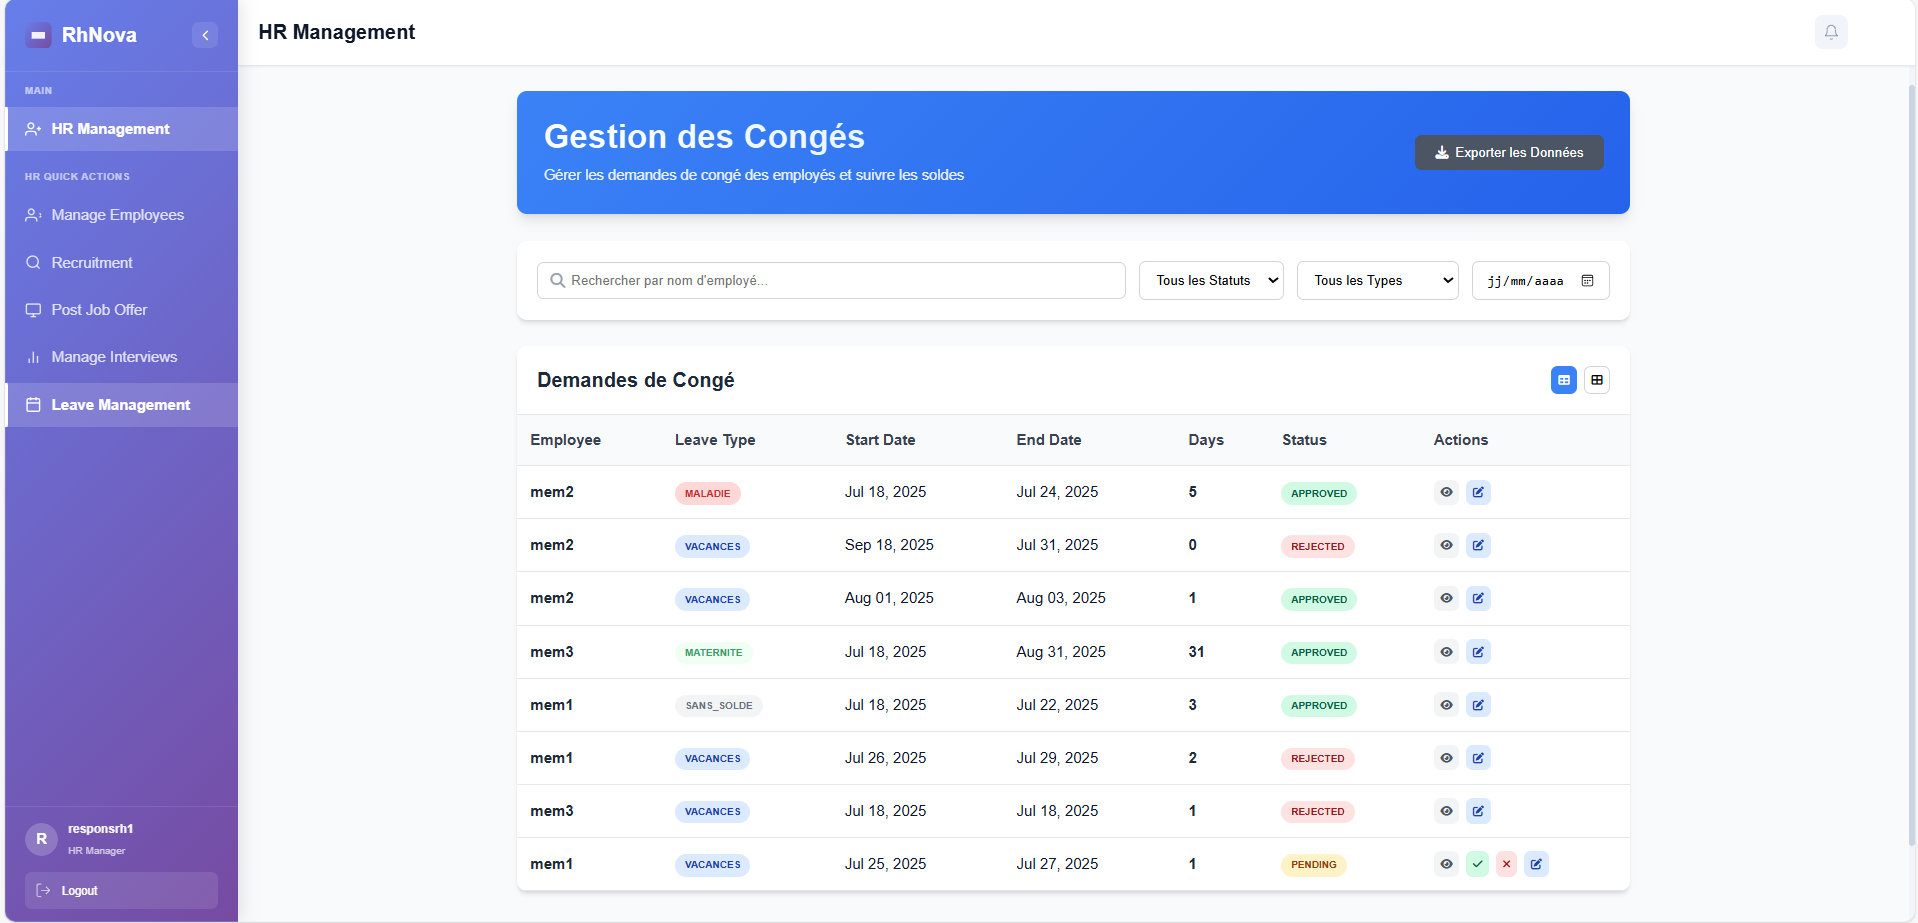
\includegraphics[width=\textwidth]{Figures/responscongé.png}
             \caption{Page de suivi des demandes congé}
         \end{figure}
              \end{itemize}
\begin{itemize}
         \item \textbf{Demande d'un congé : } Cette interface permet à un membre de l’équipe de soumettre une demande de congé en remplissant un formulaire avec le type de congé, la priorité, les dates de début et de fin, le motif et des notes éventuelles pour le manager. Elle facilite ainsi la communication et la gestion des absences au sein de l’organisation.
         
                  \begin{figure}[H]
             \centering
             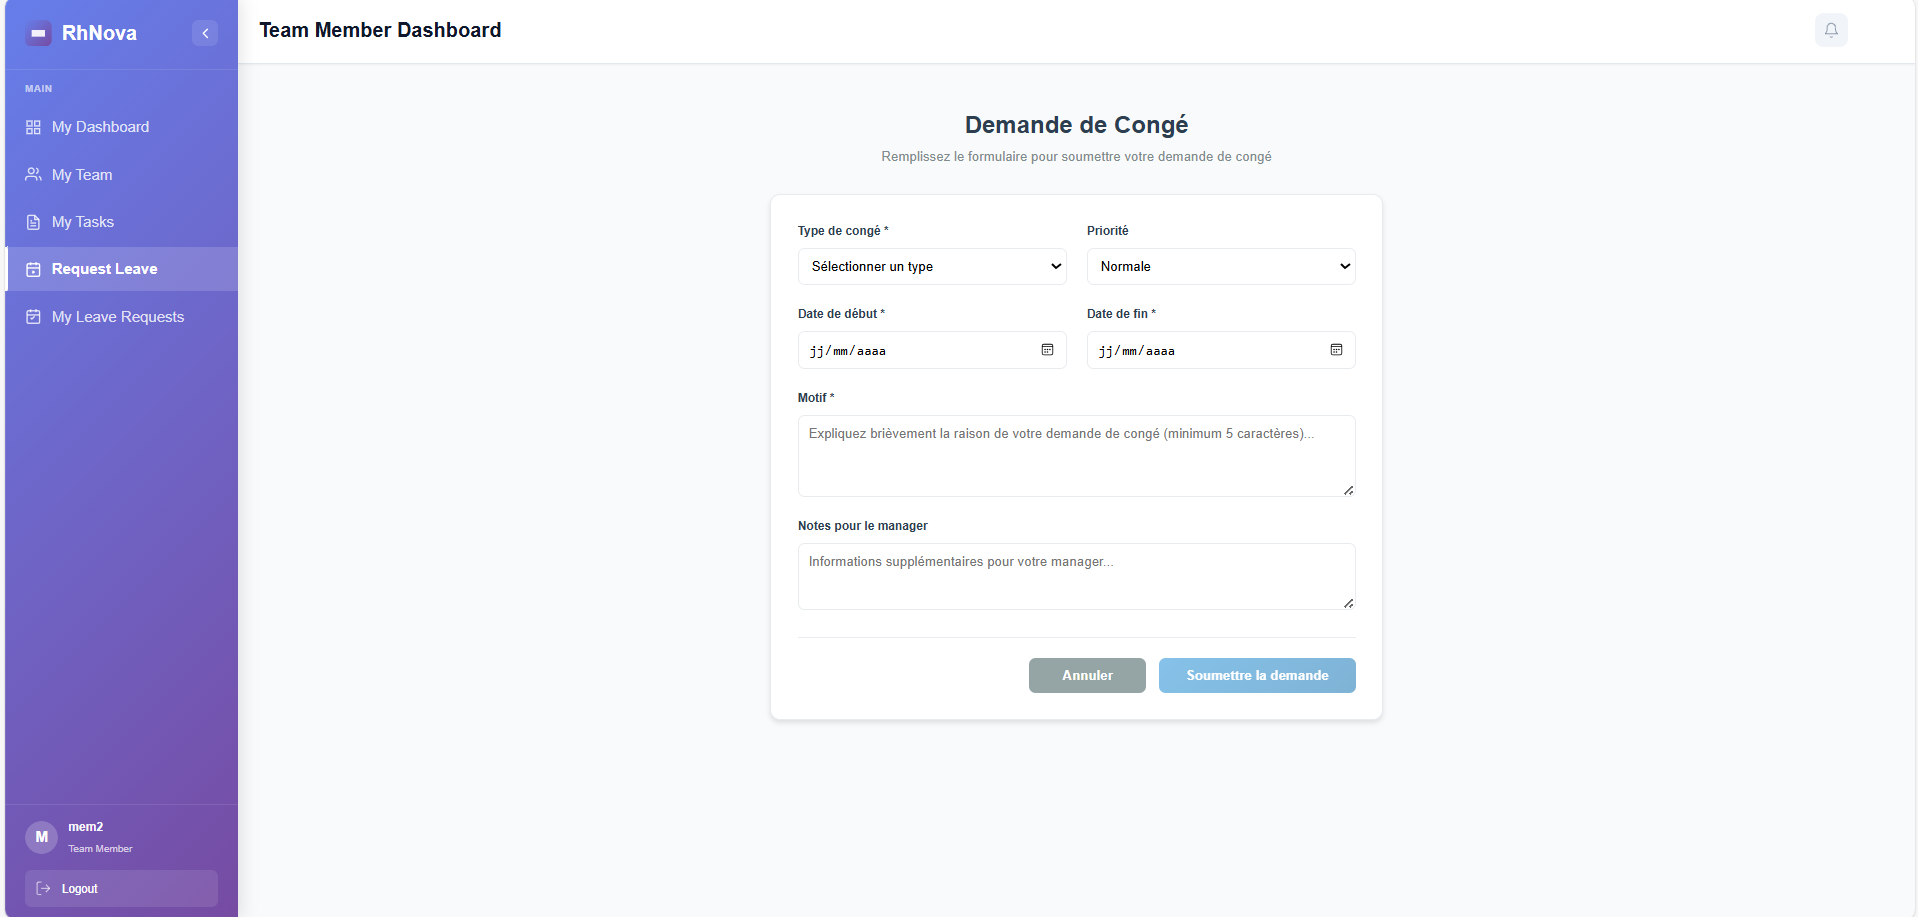
\includegraphics[width=\textwidth]{Figures/memdemande.png}
             \caption{Interface de demande de congé }
         \end{figure}
     \end{itemize}
     
\begin{itemize}
     \item\textbf{ Gestion des tâches  : }
Cette interface permet au membre d’équipe de consulter la liste des tâches qui lui ont été assignées par le manager, ainsi que leur état d’avancement et leur priorité. L’utilisateur peut également mettre à jour le pourcentage de progression ou changer le statut des tâches (en attente, en cours, terminée) afin d’assurer un meilleur suivi de son travail.
         \begin{figure}[H]
             \centering
             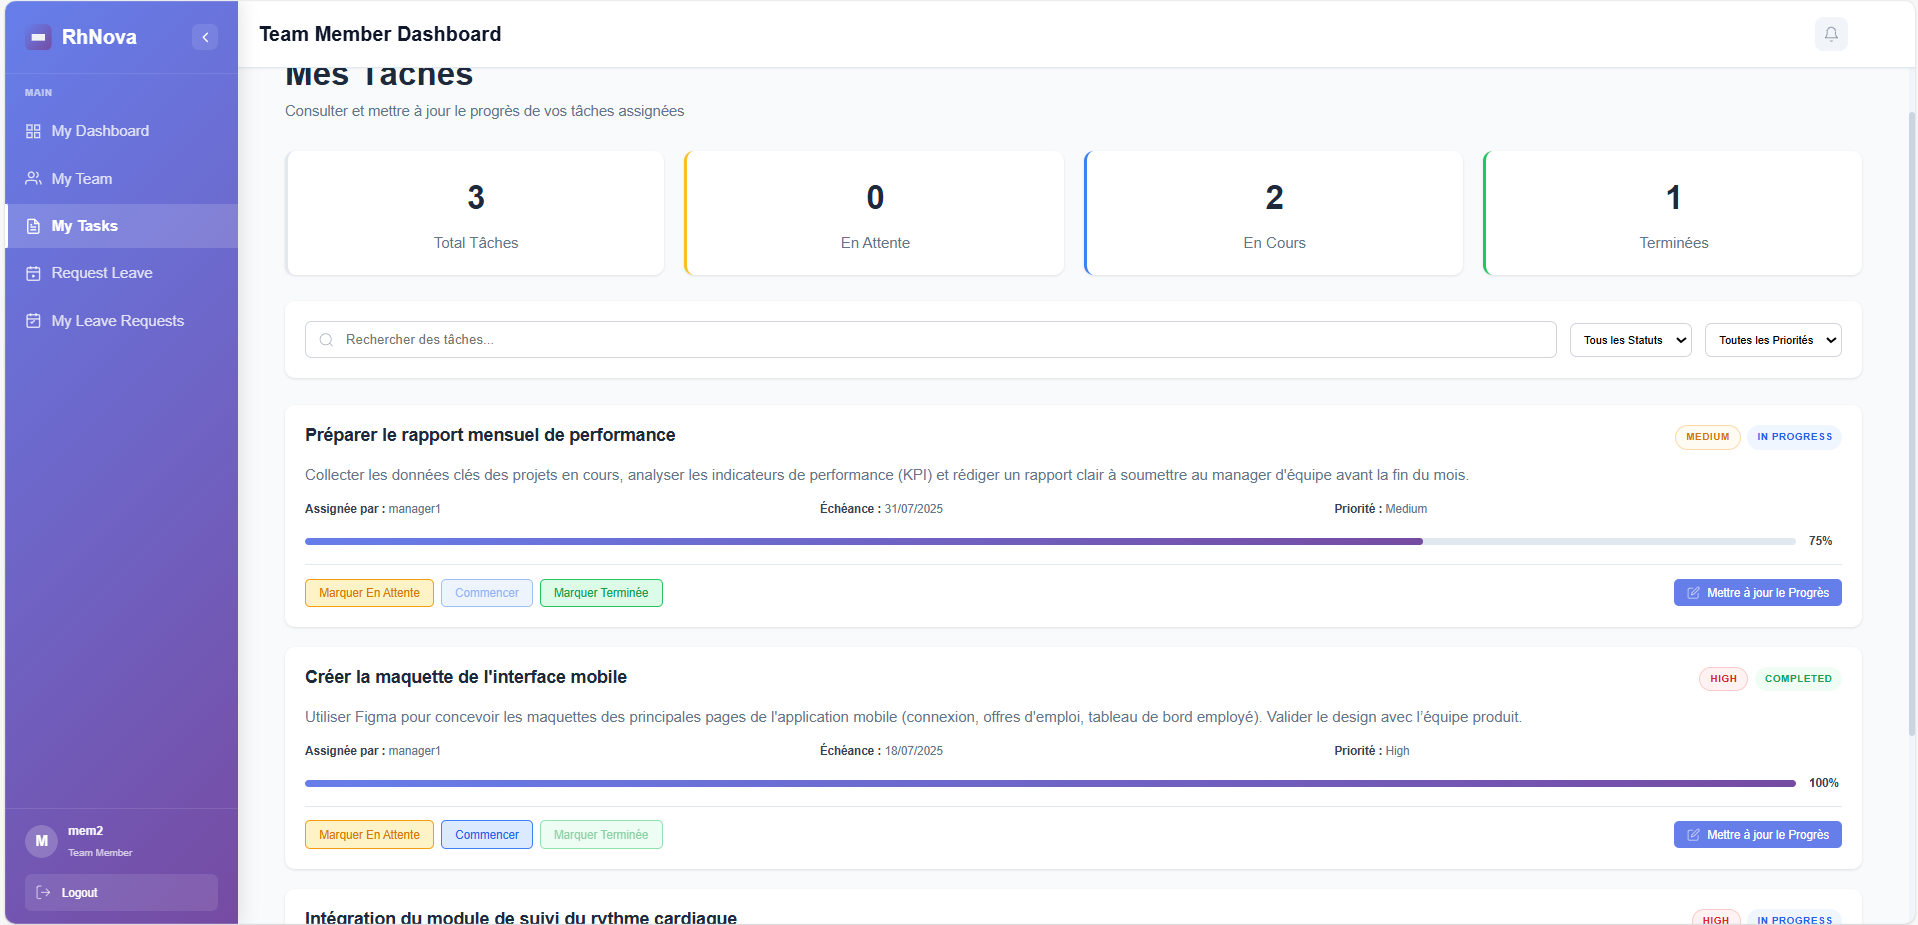
\includegraphics[width=\textwidth]{Figures/memtache.png}
             \caption{Interface de gestion des tâches }
         \end{figure}
     \end{itemize}
     
\begin{itemize}
     \item\textbf{  Consultation équipe   : }
Cette interface permet au membre d’équipe de visualiser les informations sur son équipe actuelle. Il peut voir le nom de l’équipe, son manager, la date de création, ainsi que la liste des membres avec leurs rôles et leurs adresses e-mail.     
         \begin{figure}[H]
             \centering
             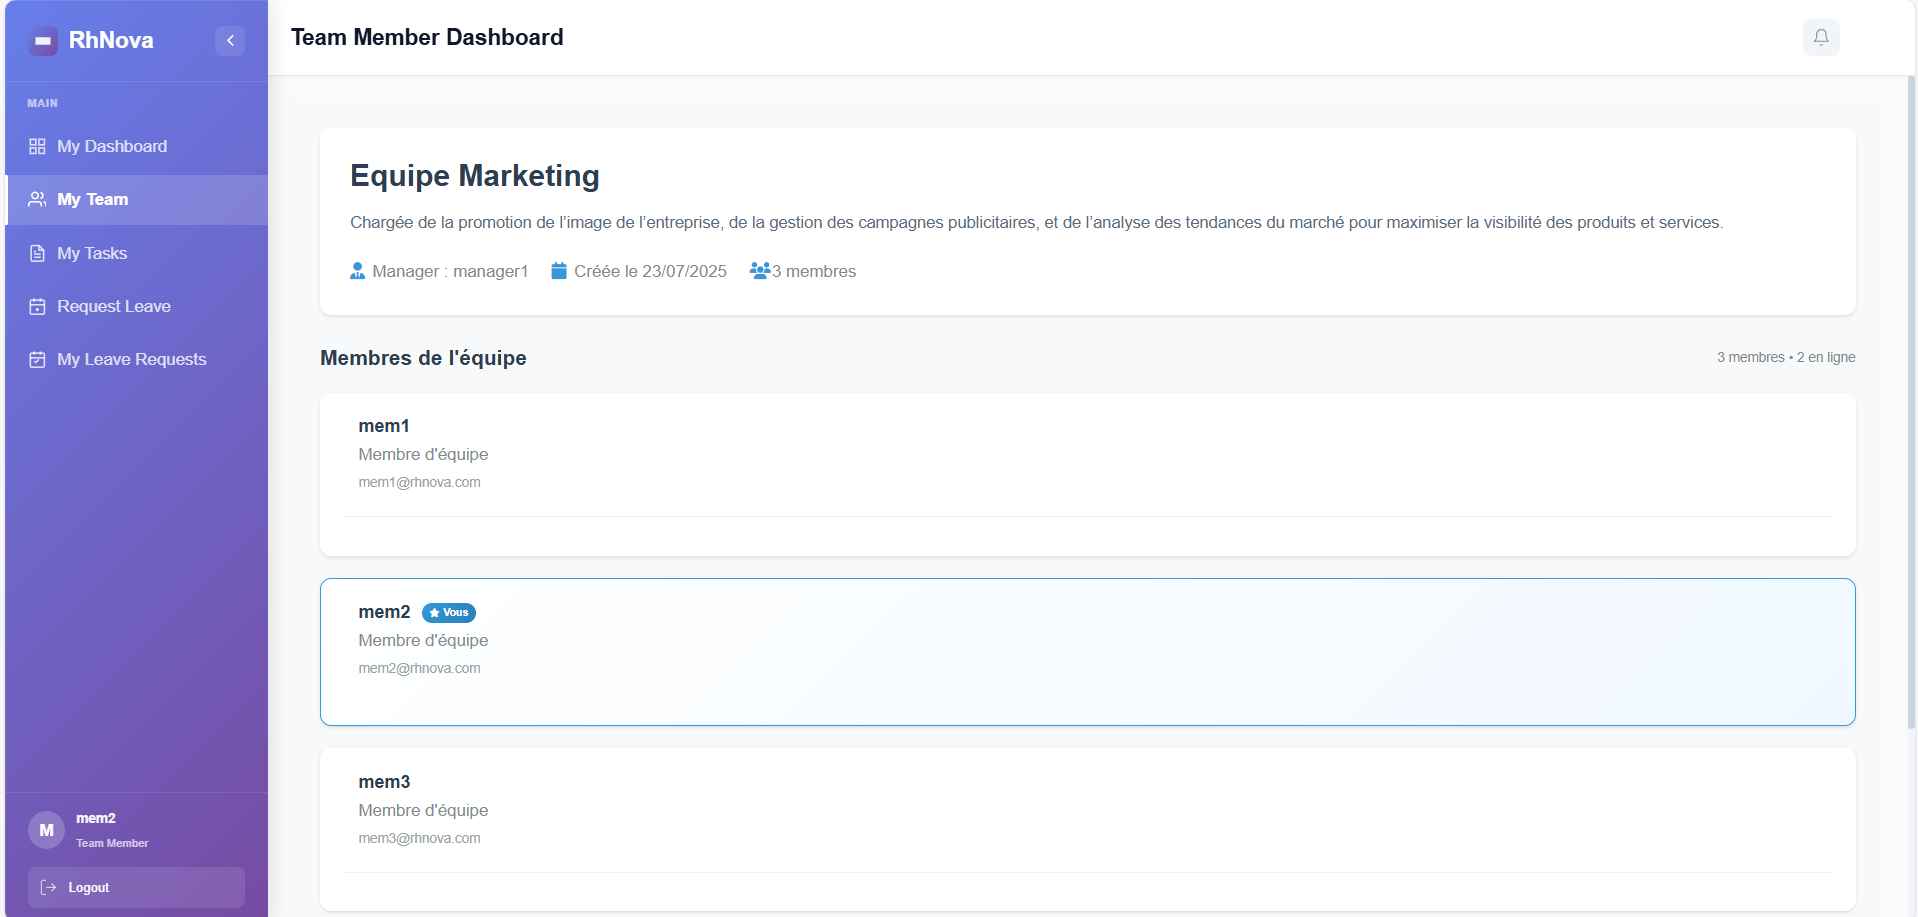
\includegraphics[width=\textwidth]{Figures/memequipe.png}
             \caption{Interface de consultation équipe }
         \end{figure}
     \end{itemize}
     
\begin{itemize}
     \item\textbf{  Consultation de l’historique des demandes de congé : }
Cette interface permet au membre d’équipe de visualiser l’historique complet de ses demandes de congé. Il peut voir le nombre de jours accordés, le statut de chaque demande (acceptée, refusée ou en attente), la période concernée, le type de congé, la raison, la date de soumission ainsi que les commentaires du manager.  
            \begin{figure}[H]
             \centering
             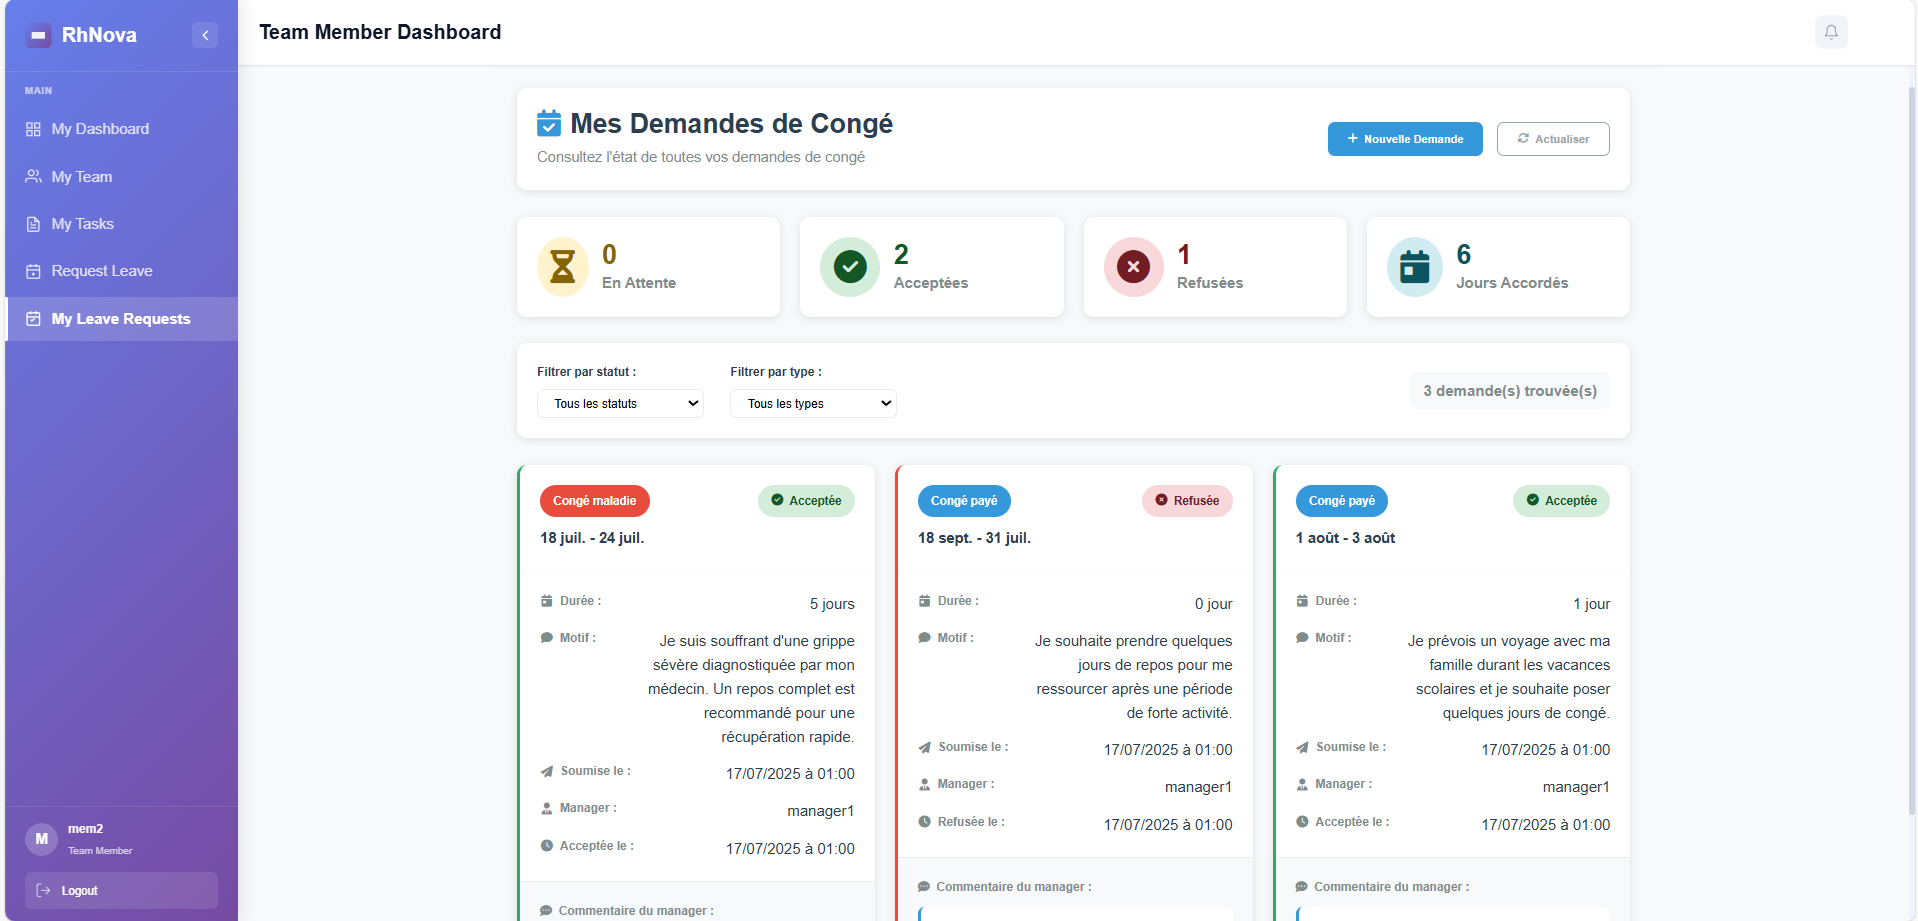
\includegraphics[width=\textwidth]{Figures/memhistorique.png}
             \caption{Interface de consultation de l’historique des demandes de congé}
         \end{figure}

     \end{itemize}
\begin{itemize}
         \item \textbf{Gestion des demandes de congé  : }Cette interface permet au manager de consulter et gérer toutes les demandes de congé soumises par les membres de son équipe. Il peut voir le détail de chaque demande (membre concerné, période, durée, motif, notes), identifier les demandes urgentes, et les approuver ou les refuser directement. 
         \begin{figure}[H]
             \centering
             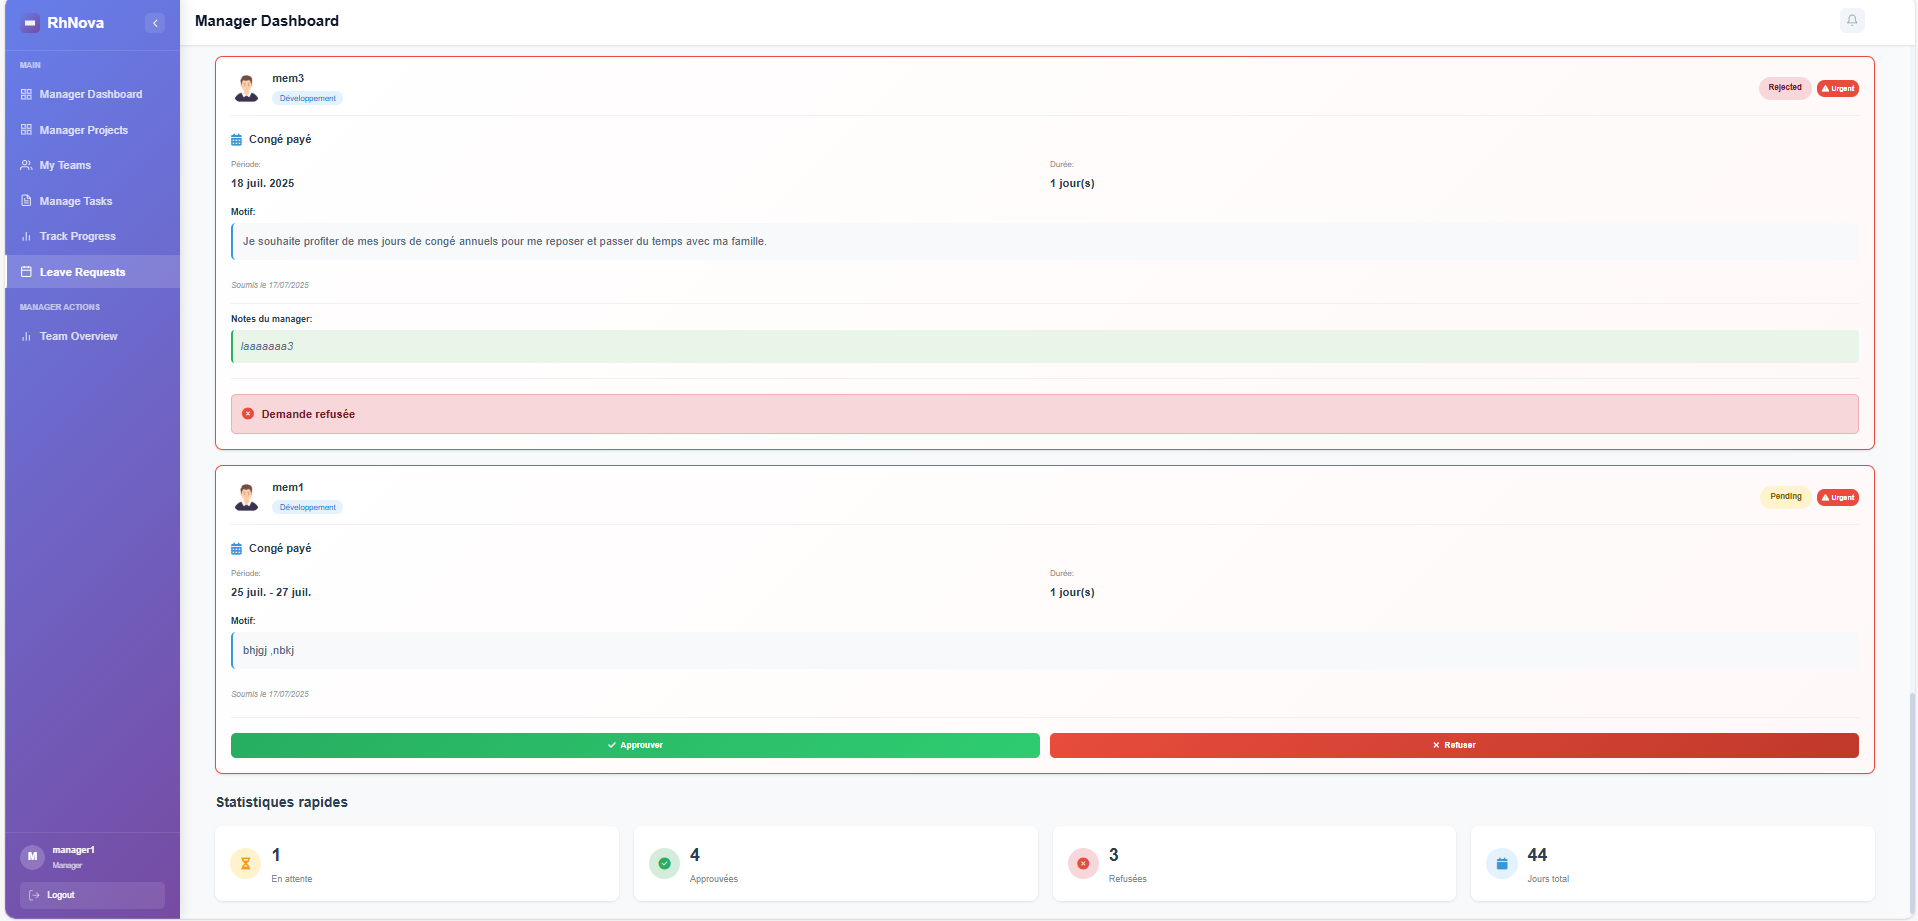
\includegraphics[width=\textwidth]{Figures/managercongé.png}
             \caption{Interface de gestion des demandes de congé }
         \end{figure}
     \end{itemize}


\section*{Conclusion}
En conclusion, ce chapitre a structuré la Sprint Gestion des Congés et Tâches, en définissant les objectifs et détaillant le backlog, tout en exposant les diagrammes de cas d’utilisation, classes et de séquences. Les descriptions textuelles et captures d’écran ont confirmé la mise en œuvre réussie, établissant un fondement solide pour la future gestion des ressources humaines.
\addcontentsline{toc}{section}{\protect\numberline{}Conclusion}%
\vspace{50mm}
\chapter*{Conclusion Générale}
\addcontentsline{toc}{chapter}{Conclusion Générale}
Ce projet de fin d’études, réalisé au sein de l’entreprise Bee Coders, a abouti au développement d’une plateforme web nommée HrNova, dédiée à la digitalisation des processus RH. Ce prototype opérationnel intègre les fonctionnalités essentielles telles que la gestion des offres d’emploi, des candidatures avec un système intelligent de filtrage de CV, la planification d’entretiens, la gestion des congés, le suivi de projet, l’organisation des tâches et la gestion des comptes utilisateurs selon différents rôles. \\
 
Développée selon une approche agile avec la méthode Scrum, cette solution nous a permis de mettre en œuvre nos compétences techniques, méthodologiques et collaboratives dans un contexte professionnel réel. Toutefois, en tant que prototype destiné à une seule entreprise, HrNova présente certaines limites, notamment l'absence d’une architecture multi-tenant et d’un module de communication interne. \\

Parmi les pistes d’amélioration envisagées, il serait pertinent d’ajouter un super administrateur capable de gérer plusieurs entreprises sur la même plateforme. Chaque entreprise pourrait être identifiée par son domaine de messagerie professionnel (par exemple, @ooredoo.com, @vermeg.com), ce qui permettrait de créer une solution RH centralisée, adaptée à un usage à plus grande échelle. D'autres évolutions possibles incluent l’ajout d’un système de messagerie instantanée interne entre les membres d’une équipe et leur manager pour favoriser la collaboration, ainsi que la mise en place d’un envoi automatique de mails aux candidats lors de la planification d’un entretien, renforçant ainsi la réactivité et la fluidité du processus de recrutement. \\



\markboth{Conclusion Générale}{}
\include{ref}
%
\section*{Résumé }



{\bf Mots clefs : } 

%To start typing in Arabic use the command arabtext
\section*{Abstract}



{\bf Keywords:} Digital 
%\setcode{utf8}
%To start typing in Arabic use the command arabtext
  
 %To start typing in Arabic use the command arabtext




 

%\include{ref}
%\include{neto}
%\tracingall
\bibliographystyle{plain}
\bibliography{allbiblio}
\end{document}